\documentclass[10pt,a4paper]{article}
\usepackage[utf8x]{inputenc}
\usepackage{ucs}
\usepackage[german]{babel}
\usepackage[left=2.00cm, right=2.00cm, top=2.00cm, bottom=2.00cm]{geometry}
\renewcommand\familydefault{\sfdefault}

\title{Zusammenfassung - Regelungstechnik}
\author{}
\date{2019}

%costum layout
\setlength{\parindent}{0cm}
\usepackage{fancyhdr}
%\usepackage{xcolor}
\pagestyle{fancy}
\fancyhf{}
\fancyhead[L]{
	\strut\rlap{\color{cyan!50!blue}\rule[-\dp\strutbox]{\headwidth}{\headheight}}
	\textcolor {white} {Zusammenfassung: Regelungstechnik}}
\fancyfoot[L]{
	\strut\rlap{\color{cyan!50!blue}\rule[-\dp\strutbox]{\headwidth}{\headheight}}
	\textcolor {white} {zuletzt aktualisiert: \today}}
\fancyhead[R]{\textcolor{white}{Sommersemester 2019}}
%\lfoot{}
\fancyfoot[R]{\textcolor{white} {\thepage}}
%\renewcommand{\footrulewidth}{1pt}

%math
\usepackage{amsmath}
\usepackage{amsfonts}
\usepackage{amssymb}
\usepackage{amstext}
\usepackage{mathtools}

%graphics
\usepackage{graphicx}
\usepackage{floatflt}
\usepackage{float}

%tabular
\usepackage{tabularx}
\usepackage[font=small,labelfont=small]{caption}
\usepackage{colortbl}
\usepackage[dvipsnames]{xcolor}
\renewcommand{\arraystretch}{1.5}
%\arrayrulecolor{white}

%tikz
\usepackage{tikz}
\usetikzlibrary{shapes, petri}
\tikzstyle{ell}=[ellipse,draw, yshift=-2mm]
\tikzstyle{rec} = [rectangle, draw]
\tikzstyle{dia} = [diamond, aspect=2, draw, yshift=-5mm]
\tikzstyle{cir} = [circle, draw, minimum size=3mm]
\tikzstyle{arrHV} = [to path={-| (\tikztotarget)}]
\tikzstyle{arrVH} = [to path={|- (\tikztotarget)}]
\tikzstyle{whileright} = [xshift=20mm, yshift=-3mm]
\tikzstyle{whileleft} = [xshift=-20mm, yshift=-3mm]
\tikzstyle{txtright} = [above, xshift=15mm]
\tikzstyle{txtleft} = [above, xshift=-15mm]
\tikzstyle{empty} = [coordinate]
\usetikzlibrary{positioning}

%listings
\usepackage{listings}
\lstdefinestyle{costum} {
	language=Bash,
	basicstyle=\footnotesize\ttfamily,
	keywordstyle=\bfseries\color{cyan!50!blue},
	commentstyle=\itshape\color{black!50},
	%identifierstyle=\color{blue},
	stringstyle=\color{green!50!black},
	morekeywords={returns, loop, each},
	escapeinside={\%*}{*)}
}
\lstset{style=costum}

%multicol
\usepackage{multicol}
%\setlength{\columnseprule}{0pt}
%\setlength{\columnsep}{20.0pt}



%custom title color
\usepackage{titlesec}
%\titleformat{\section}
%{\color{cyan!80!blue}\normalfont\Large\bfseries}
%{\color{black}\thesection}{1em}{}

%\titleformat{\subsubsection}
%{\color{blue!30!black!70}\normalfont\bfseries}
%{\color{black}\thesection}{1em}{}

\setcounter{secnumdepth}{4}

%\titleformat{\paragraph}
%{\color{green!30!black!70}\normalfont\normalsize\bfseries}{\theparagraph}{1em}{}
%\titlespacing*{\paragraph}
%{0pt}{3.25ex plus 1ex minus .2ex}{1.5ex plus .2ex}

%tab
\newcommand{\tab}[1][1]{\hspace*{#1cm}}

%color_summary
\newcommand{\sumcolor}[1]{\textcolor{red!10!green!40!blue}{#1}}

%coloring
\newcommand{\redr}{\textcolor{red}{r}}
\newcommand{\greeng}{\textcolor{green}{g}}
\newcommand{\blueb}{\textcolor{blue}{b}}

%vector
\newcommand{\vect}[1]{\ensuremath{\begin{bmatrix}#1\end{bmatrix}}}

%other
\usepackage{enumerate}
\usepackage{hyperref}
\usepackage{mathpartir}
\usepackage{trfsigns}
\usepackage{multicol}


%TODO
% Hinweise:
% -----
% Ruhelage
% Partialbruchzerlegung
%
% Fix:
% ---
% 2.1.1 Blockschaltbild P-Glieder



\begin{document}
	\tableofcontents
	\pagebreak
	
\section{Begriff der Regelung}

\subsection{Dynamisches System}
\subsubsection*{Signale und Blöcke:}
\begin{tabularx}{\columnwidth}{llX}
	Bezeichnung & Var. & Beschreibung \\
	\hline
	Ausgangsgröße & $y(t)$ & Ausgangsgröße, der ein gewünschtes Verhalten aufgeprägt werden soll \\
	Stellgröße & $u(t)$ & Eingangsgröße, durch die das System gezielt beeinflusst werden kann \\
	Störgröße & $z(t)$ & Eingangsgröße, die störend und mit zumeist nur ungenau oder gar nicht bekannten Zeitverlauf auf das System wirkt \\
\end{tabularx}

\subsubsection*{Blockschaltbild}
\begin{figure}[H]
	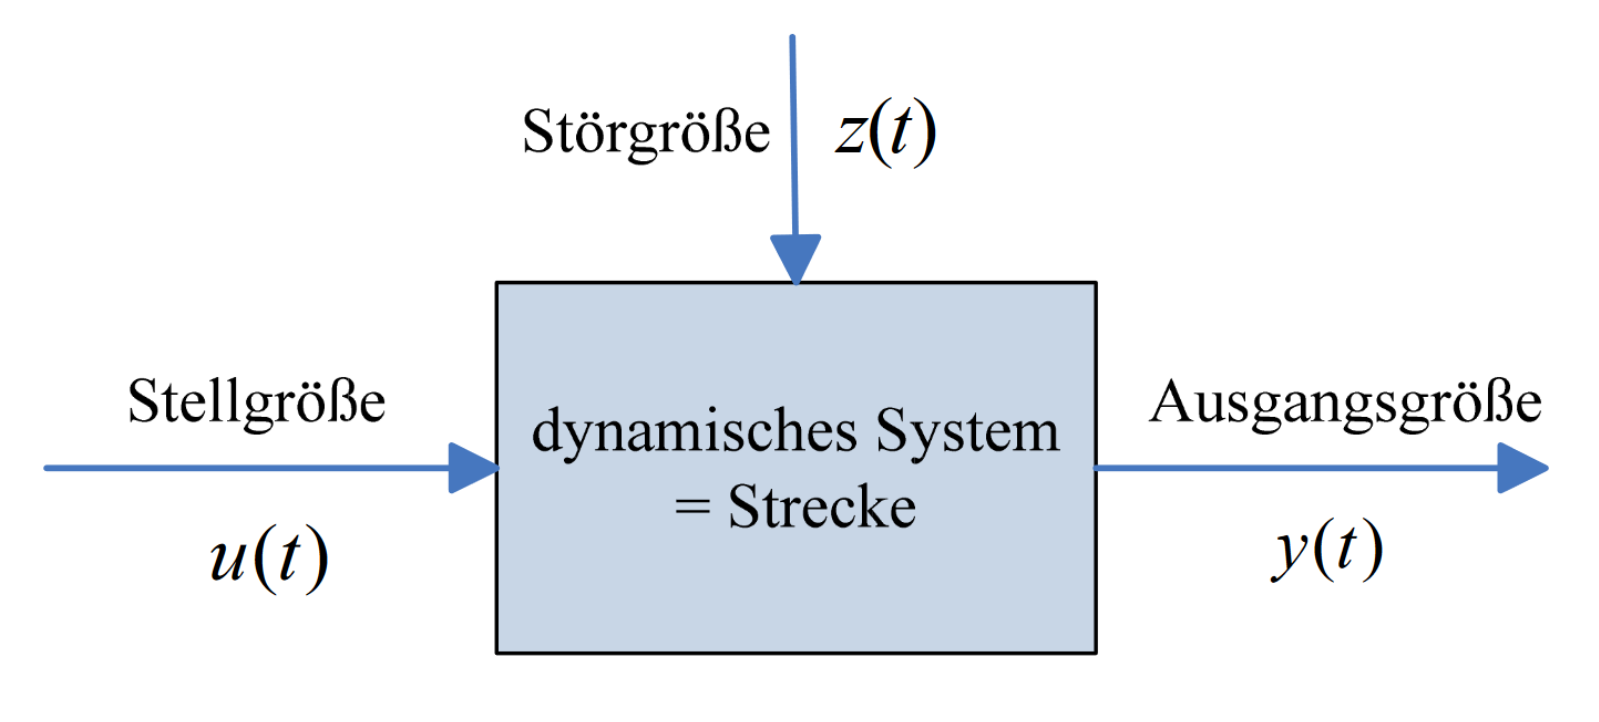
\includegraphics[width=0.5\columnwidth]{imgs/abb1_3.png}
\end{figure}

\subsection{Vorgeschaltete Steuereinrichtung}
\label{steuerung}
\subsubsection*{Ziel}
\begin{itemize}
	\item Übertragungsglied, das den Stellgrößenverlauf $u(t)$ derart generiert, dass $y(t)$ einem vorgegebenen Sollverlauf $w(t)$ folgt.
\end{itemize}

\subsubsection*{Signale und Blöcke:}
\begin{tabularx}{\columnwidth}{llX}
	Bezeichnung & Var. & Beschreibung \\
	\hline
	Führungsgröße & $w(t)$ & Von außen vorgegebener Soll-Verlauf für die Regelgröße y(t) \\
	Ausgangsgröße & $y(t)$ & Ausgangsgröße, der ein gewünschtes Verhalten aufgeprägt werden soll \\
	Stellgröße & $u(t)$ & Eingangsgröße, durch die das System gezielt beeinflusst werden kann \\
	Störgröße & $z(t)$ & Eingangsgröße, die störend und mit zumeist nur ungenau oder gar nicht bekannten Zeitverlauf auf das System wirkt \\
\end{tabularx}

\subsubsection*{Blockschaltbild}
\begin{figure}[H]
	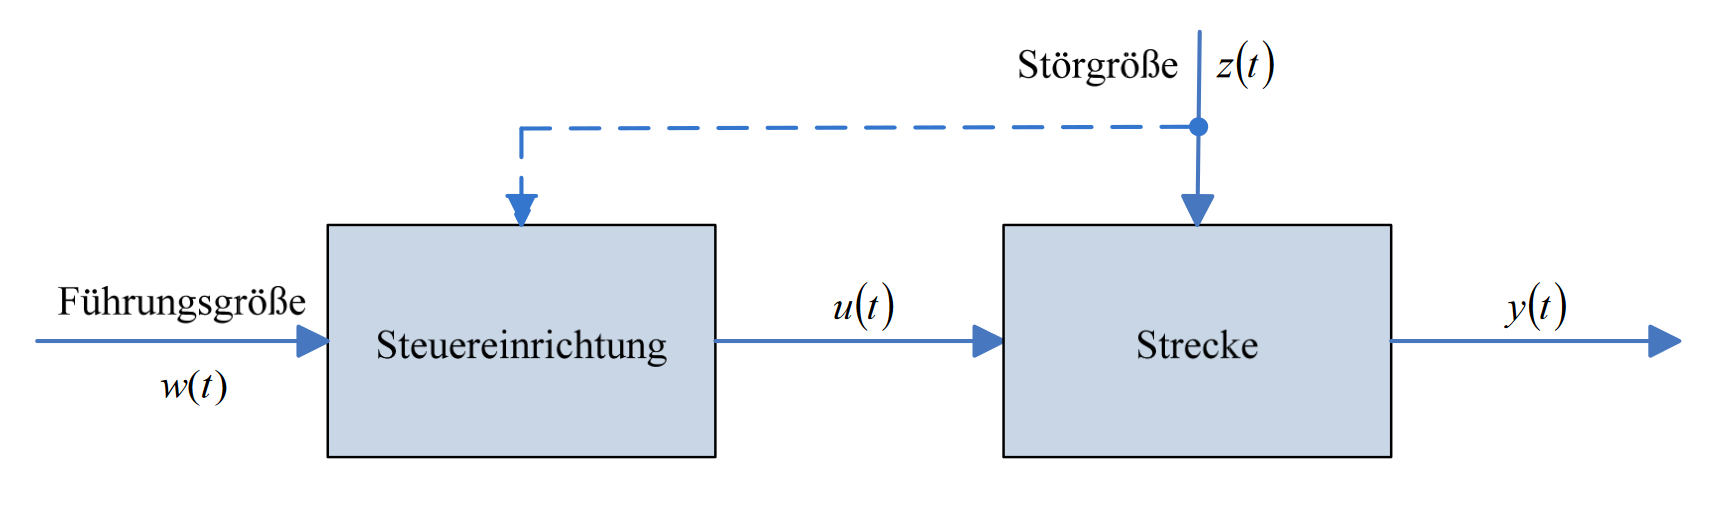
\includegraphics[width=0.8\columnwidth]{imgs/abb1_4.png}
\end{figure}


\subsection{Regelung}
\label{regelung}
\subsubsection*{Ziel:}
\begin{itemize}
		\item Minderung des Einflusses von (nicht-messbaren) Störungen
		\item Minderung des Einflusses von Ungenauigkeiten des Streckenmodells
		\item Verbesserung des Folgeverhaltens
\end{itemize}

\subsubsection*{Signale und Blöcke:}

\begin{tabularx}{\columnwidth}{llX}
	Bezeichnung & Var. & Beschreibung \\
	\hline
	Führungsgröße & $w(t)$ & Von außen vorgegebener Soll-Verlauf für die Regelgröße y(t) \\
	Regelgröße & $y(t)$ & Ausgangsgröße, der ein gewünschtes Verhalten aufgeprägt werden soll \\
	Regelabweichung & $e(t)$ & Entsteht durch Vergleich der Führungsgröße mit der gemessenen Regelgröße und soll klein gehalten werden ($e(t) = w(t) - y'(t)$) \\
	Stellgröße & $u(t)$ & Eingangsgröße, durch die das System gezielt beeinflusst werden kann \\
	Störgröße & $z(t)$ & Eingangsgröße, die störend und mit zumeist nur ungenau oder gar nicht bekannten Zeitverlauf auf das System wirkt \\
	Messrauschen & $n(t)$ & \\
	Regler && Übertragungsglied, das aus der Regelabweichung das Stellsignal $u$ generiert, sodass $y$ möglichst $w$ folgt \\
	Messglied/Messeinrichtung && Erfasst die Regelgröße $y$ mittels eines Sensors und erzeugt ein zu $y(t)$ möglichst äquivalentes Signal $y'(t)$	
\end{tabularx}

\subsubsection*{Blockschaltbild}
\begin{figure}[H]
	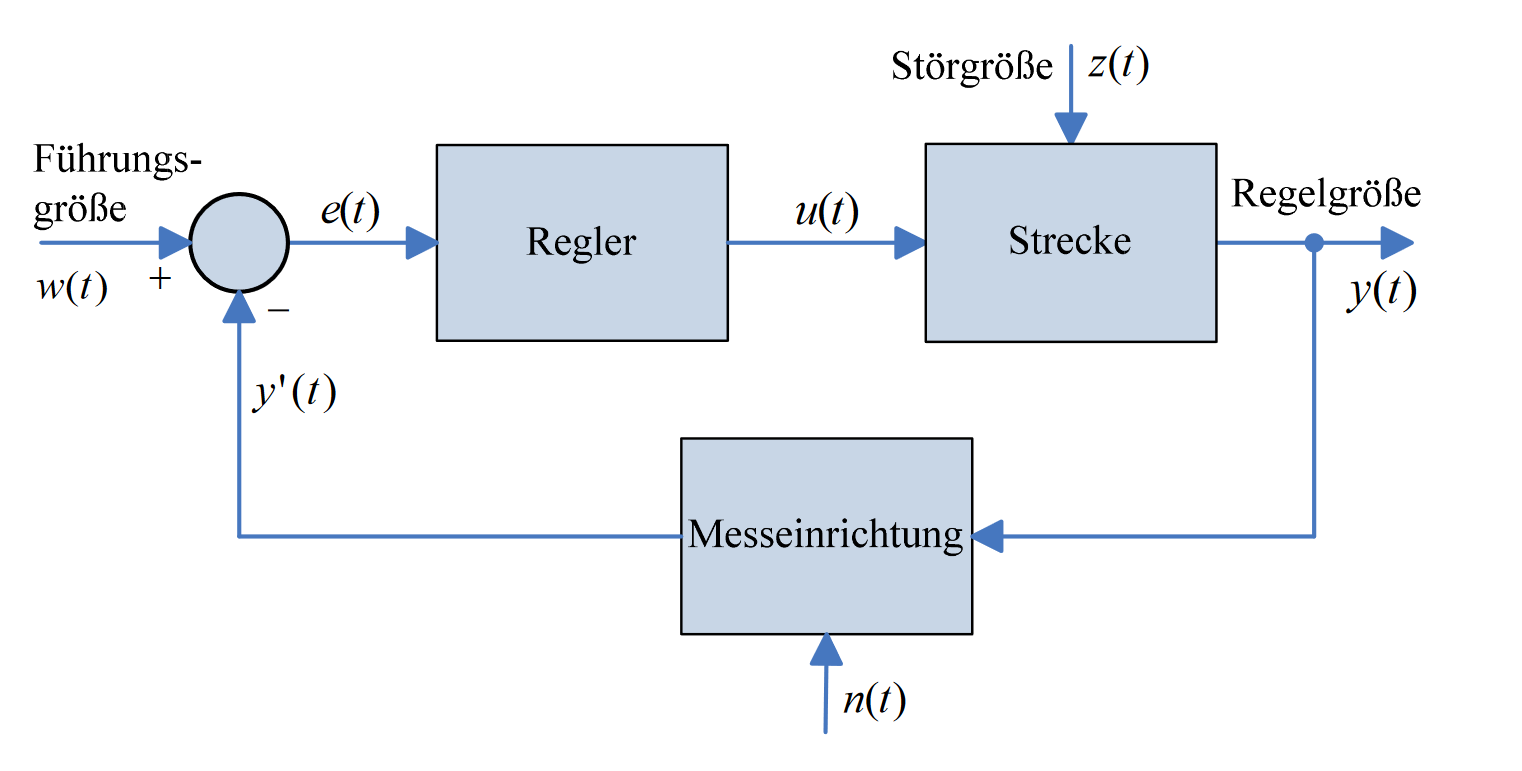
\includegraphics[width=0.8\columnwidth]{imgs/abb1_6.png}
\end{figure}


\subsection{Zwei-Freiheitsgrade-Regelung (Steuerung + Regelung)}
\subsubsection*{Ziel:}
\begin{itemize}
		\item Kombination der Vorteile der Regelschleife (see section \ref{regelung}) und der Vorteile der Steuerung (see section \ref{steuerung})
\end{itemize}

\subsubsection*{Signale und Blöcke:}

\begin{tabularx}{\columnwidth}{llX}
	Bezeichnung & Var. & Beschreibung \\
	\hline
	Führungsgröße & $w(t)$ & Von außen vorgegebener Soll-Verlauf für die Regelgröße y(t) \\
	Regelgröße & $y(t)$ & Ausgangsgröße, der ein gewünschtes Verhalten aufgeprägt werden soll \\
	Regelabweichung & $e(t)$ & Entsteht durch Vergleich der Führungsgröße mit der gemessenen Regelgröße und soll klein gehalten werden ($e(t) = w(t) - y'(t)$) \\
	Stellgröße & $u(t)$ & Eingangsgröße, durch die das System gezielt beeinflusst werden kann \\
	Störgröße & $z(t)$ & Eingangsgröße, die störend und mit zumeist nur ungenau oder gar nicht bekannten Zeitverlauf auf das System wirkt \\
	Regler && Übertragungsglied, das aus der Regelabweichung das Stellsignal $u$ generiert, sodass $y$ möglichst $w$ folgt \\
	Steuereinrichtung && Übertragungsglied, das den Stellgrößenverlauf $u(t)$ derart generiert, dass $y(t)$ einem vorgegebenen Sollverlauf $w(t)$ folgt.
\end{tabularx}

\subsubsection*{Blockschaltbild}
\begin{figure}[H]
	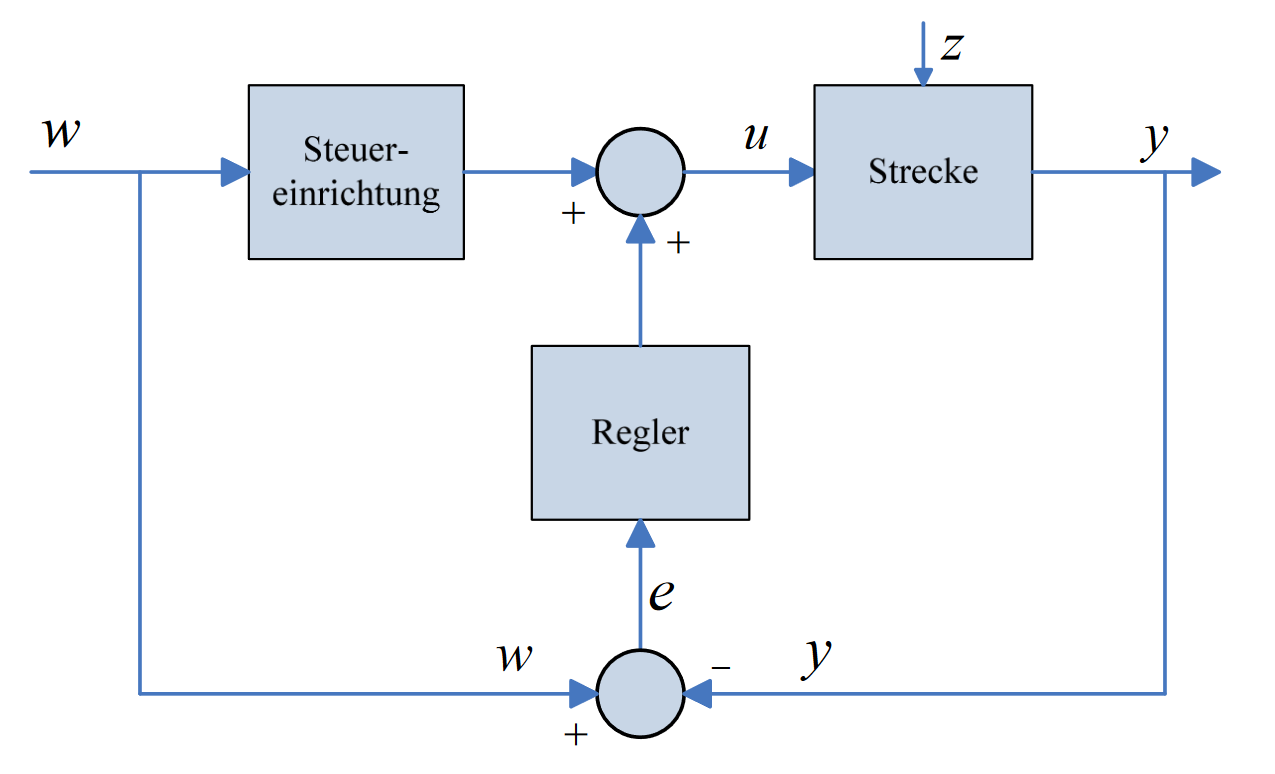
\includegraphics[width=0.8\columnwidth]{imgs/abb1_8.png}
\end{figure}

%TODO evtl Blockschaltbild mit Trajectorienplaner

\subsubsection{Störgrößenaufschaltung}
\subsubsection*{Ziel:}
\begin{itemize}
	\item Mindern des Einflusses einer messbaren Störgröße auf den Ausgang
\end{itemize}

\subsubsection*{Signale und Blöcke:}
\begin{tabularx}{\columnwidth}{llX}
	Bezeichnung & Var. & Beschreibung \\
	\hline
	Führungsgröße & $w(t)$ & Von außen vorgegebener Soll-Verlauf für die Regelgröße y(t) \\
	Regelgröße & $y(t)$ & Ausgangsgröße, der ein gewünschtes Verhalten aufgeprägt werden soll \\
	Regelabweichung & $e(t)$ & Entsteht durch Vergleich der Führungsgröße mit der gemessenen Regelgröße und soll klein gehalten werden ($e(t) = w(t) - y'(t)$) \\
	Stellgröße & $u(t)$ & Eingangsgröße, durch die das System gezielt beeinflusst werden kann \\
	Störgröße & $z_1(t)$ & Messbare Eingangsgröße, die störend auf das System wirkt \\
	Störgröße & $z_2(t)$ & Nicht-Messbare Eingangsgröße, die störend auf das System wirkt \\
	Regler && Übertragungsglied, das aus der Regelabweichung das Stellsignal $u$ generiert, sodass $y$ möglichst $w$ folgt \\
	Steuereinrichtung && Übertragungsglied, das den Stellgrößenverlauf $u(t)$ derart generiert, dass $y(t)$ einem vorgegebenen Sollverlauf $w(t)$ folgt. Besteht aus Störgrößenaufschaltung und Führungsgrößenaufschaltung \\
	Störgrößenaufschaltung && Übertragungspfad zur Aufschaltung einer messbaren Störgröße auf die Stellgröße \\
	Führungsgrößenaufschaltung && Übertragungspfad zur Aufschaltung der Führungsgröße auf die Stellgröße
\end{tabularx}

\subsubsection*{Blockschaltbild}
\begin{figure}[H]
	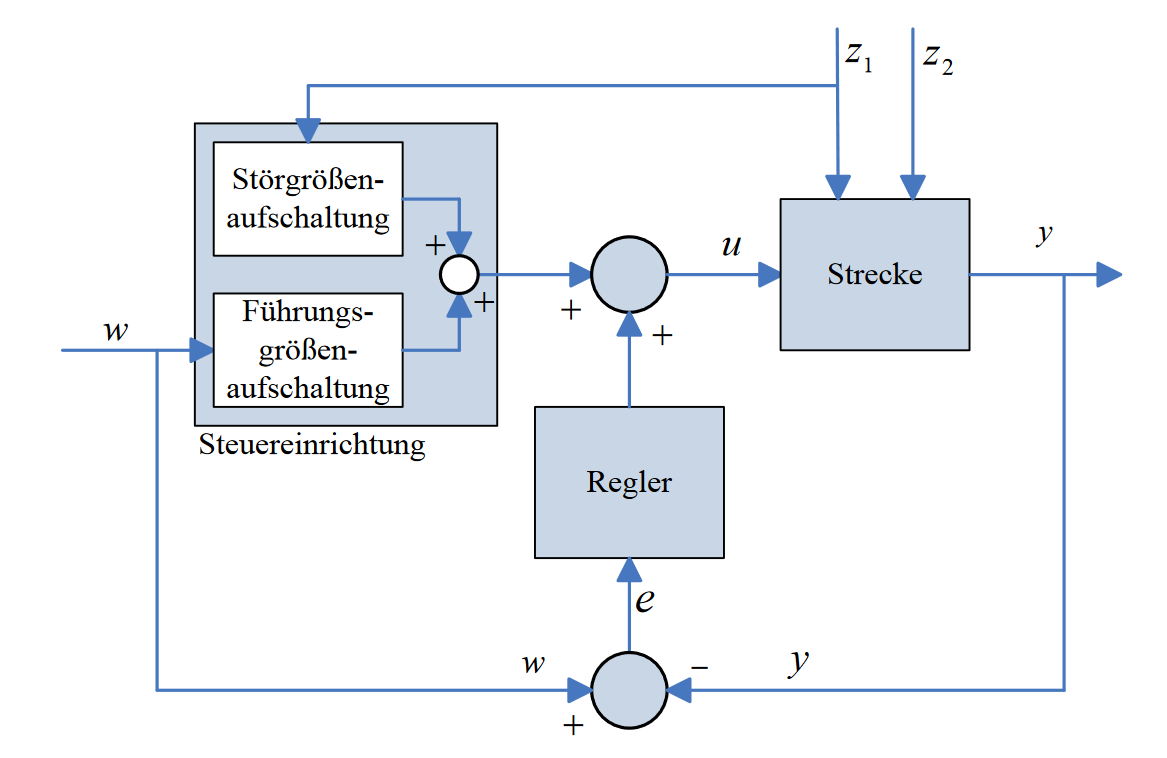
\includegraphics[width=0.8\columnwidth]{imgs/abb1_11.png}
\end{figure}

\section{Modelle}
\subsection{Zustandsdarstellung}
\renewcommand{\arraystretch}{2}
\begin{tabularx}{\columnwidth}{lX}
	Zustandsdarstellung/Zustandsraummodell & Ein Modell bestehend aus
	$$
		\begin{array}{ll}
			\begin{rcases}
				\dot x_1 = f_1(x_1 \dots x_n, z, u) \\
				\tab \vdots \\
				\dot x_n = f_n(x_1 \dots x_n, z, u)
			\end{rcases} & \text{Zustandsdifferentialgleichungen} \\
			y = g(x_1 \dots x_n) & \text{Ausgangsgleichung}
		\end{array}
	$$
	\text{bzw.} 
	$$
		\begin{array}{l}
			\dot{x} = f(x,z,u) \\
			y = g(x)
		\end{array}		
	$$
	wenn bei bekannten Eingangssignalen $u(t)$ und $z(t)$ und gegebenen Anfangswerten $x_1(0), \dots, x_n(0)$ die Zeitverläufe $x_1(t), \dots, x_n(t)$ für $t > 0$ eindeutig bestimmt sind. \\
	Zustandsgleichungen & Zustandsdifferentialgleichungen und die Ausgangsgleichung zusammen \\
	Trajektorie & Die $n$ Zeitverläufe $x_1(t), \dots, x_n(t)$ \\
	Zustandsvariablen & $x_1, \dots, x_n$ \\
	Zustand des Systems & Die Gesamtheit der Werte $x_1, \dots, x_n$ zu einem festen Zeitpunkt $t$ \\
	Zustandsvektor & 
	$$
		x(t) = \vect{x_1(t) \\ \vdots \\ x_n(t)}
	$$	
\end{tabularx}
\renewcommand{\arraystretch}{1.5}

\subsubsection{Zustandsdarstellung bei Linearkombinationen}
Bestehen die rechten Seiten der Zustandsgleichungen ausschließlich aus Linearkombinationen, d.h.:
$$
\begin{array}{l}
	\dot x_1 = a_{11} x_1 + \dots + a_{1n} x_n + e_1 z + b_1 u \\
	\tab \vdots \\
	\dot x_n = a_{n1} x_1 + \dots + a_{nn} x_n + e_n z + b_n u \\
	y = c_1 x_1 + \dots + c_n x_n
\end{array}	
$$
so gilt:
$$
\begin{array}{lcl}
	\dot{x} = A x + e z + b u & ≡ & \vect{\dot x_1 \\ \vdots \\ \dot x_n} = \vect{a_{11} & \dots & a_{1n} \\ \vdots & \ddots & \vdots \\ a_{n1} & \dots & a_{nn}} \vect{x_1 \\ \vdots \\ x_n} + \vect{e_1 \\ \vdots \\ \dot e_n} z(t) + \vect{b_1 \\ \vdots \\ \dot b_n} u(t) \\
	y = c^Tx & ≡ & y = \vect{c_1 & \dots & c_n} \vect{x_1 \\ \vdots \\ x_n}
\end{array}
$$

\paragraph*{Blockschaltbild:} ~\\
\begin{figure}[H]
	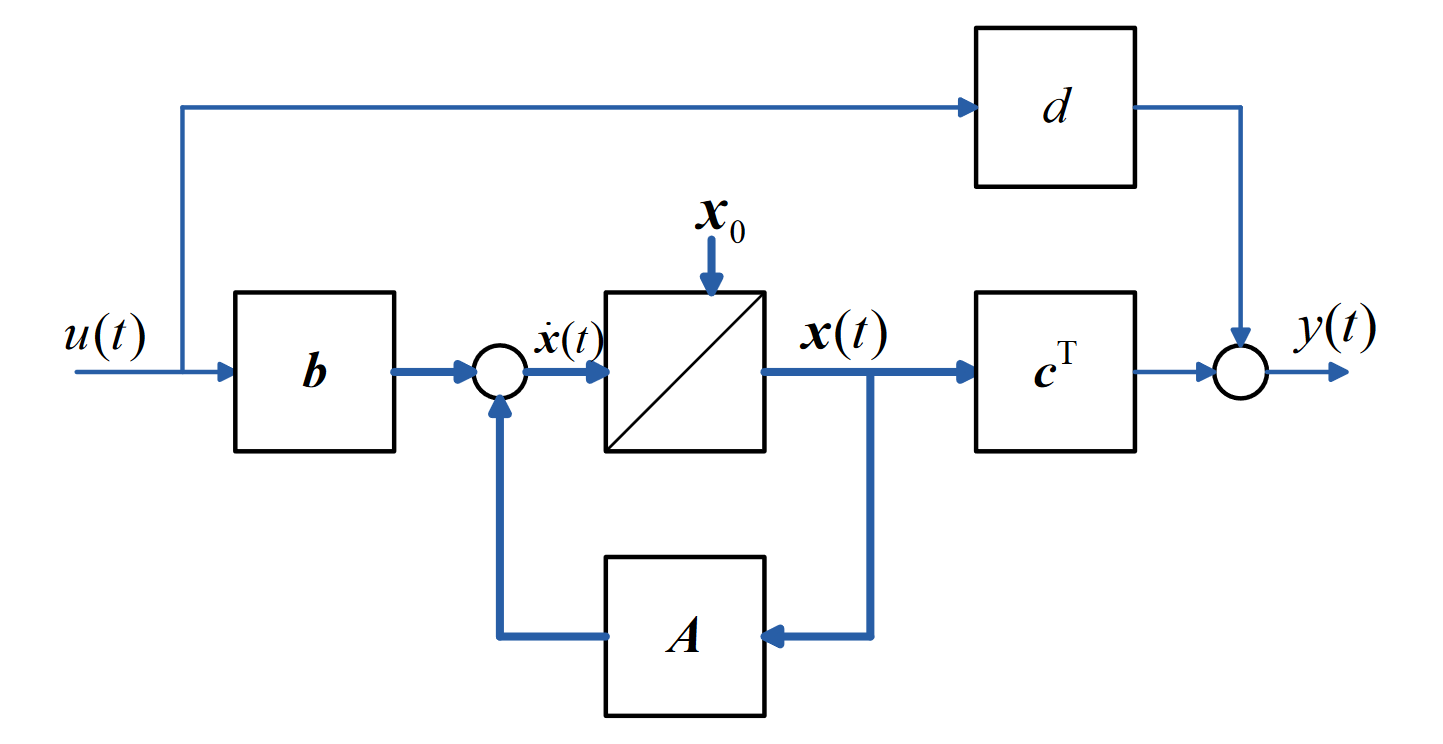
\includegraphics[width=0.8\columnwidth]{imgs/abb2_12.png}
\end{figure}

\subsection{Blockschaltbild}
\subsubsection*{Funktion:}
\begin{itemize}
	\item Das Blockschaltbild ist eine graphische Darstellung der Funktionsbeziehungen zwischen den zeitveränderlichen Größen durch Blöcke und Wirkungslinien. Ein Block ordnet dabei jedem Zeitverlauf der Eingangsgröße eindeutig einen Zeitverlauf der Ausgangsgröße zu und wirkt so als Übertragungsglied.
	Die Zuordnungsvorschrift wird dabei in den Block hineingeschrieben.
\end{itemize}

\subsubsection*{Blockschaltbild:} ~\\
\begin{figure}[H]
	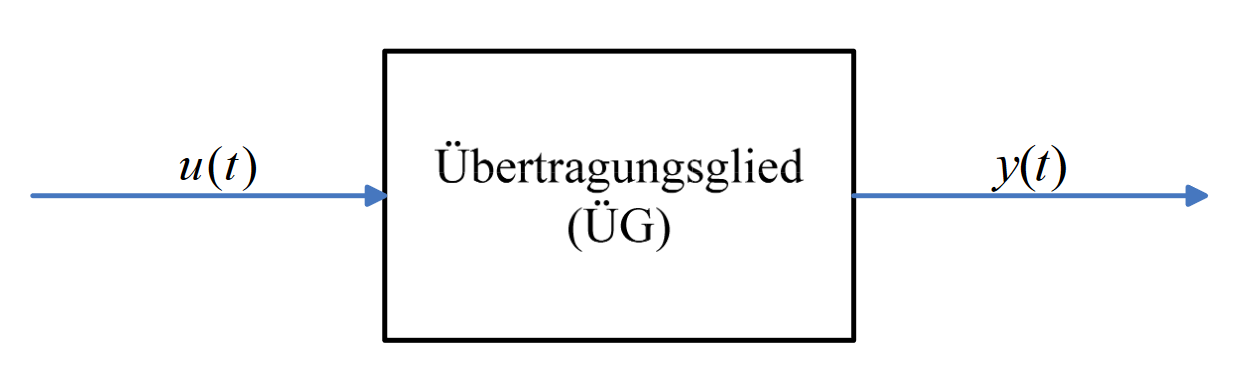
\includegraphics[width=0.8\columnwidth]{imgs/abb2_4.png}
\end{figure}

\subsection{Elementare Übertragungsglieder}
\textbf{Summationsglied:}
\begin{figure}[H]
	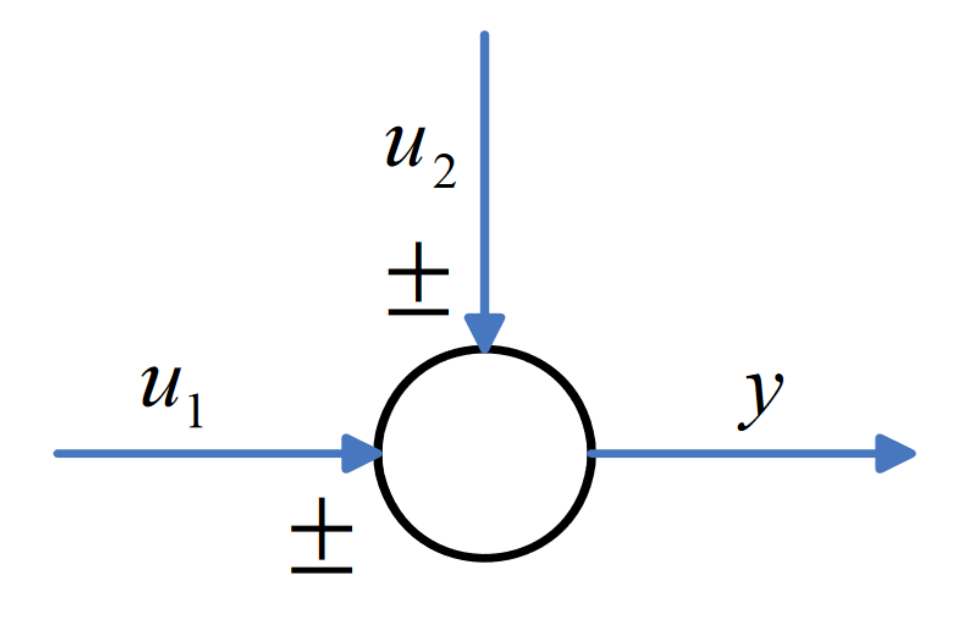
\includegraphics[width=0.2\columnwidth]{imgs/sumglied.png}
\end{figure}

\textbf{Weitere Übertragungsglieder:}
\begin{figure}[H]
	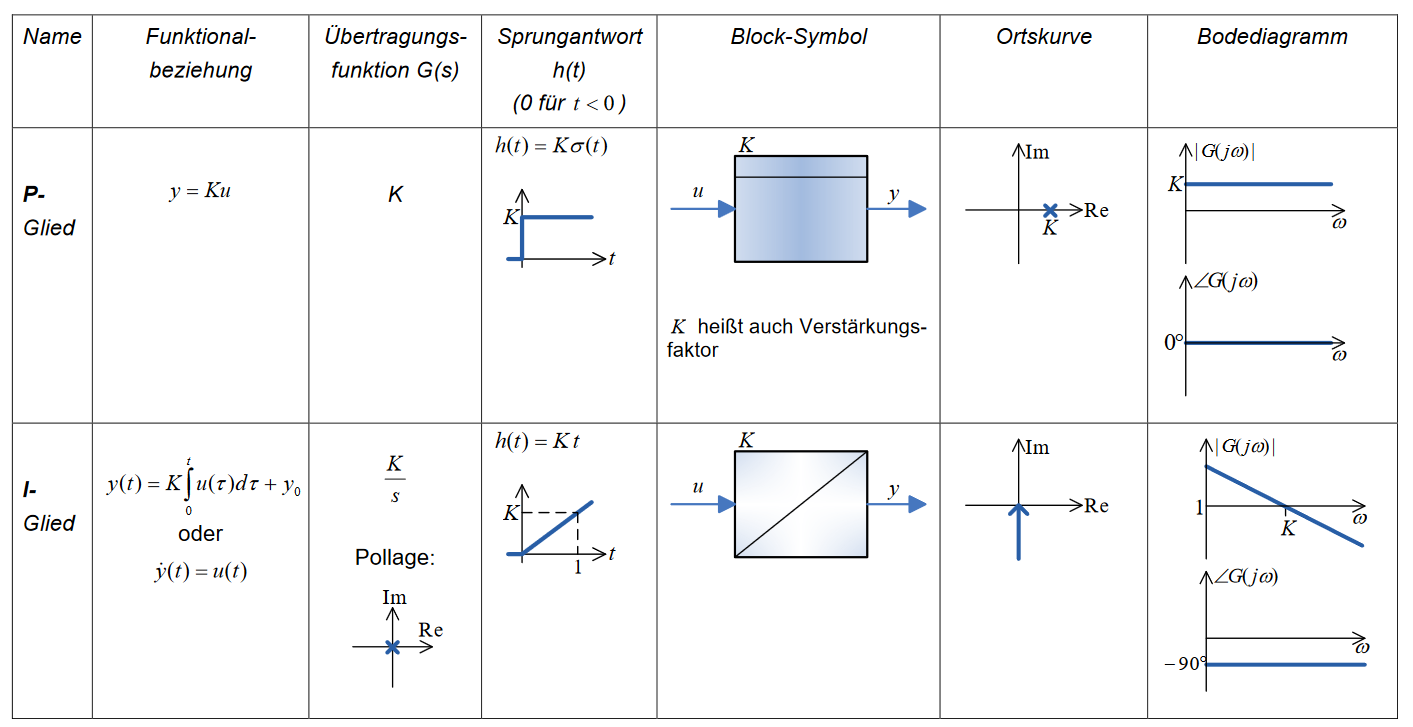
\includegraphics[width=1\columnwidth]{imgs/bb2_2a.png}
\end{figure}
\begin{figure}[H]
	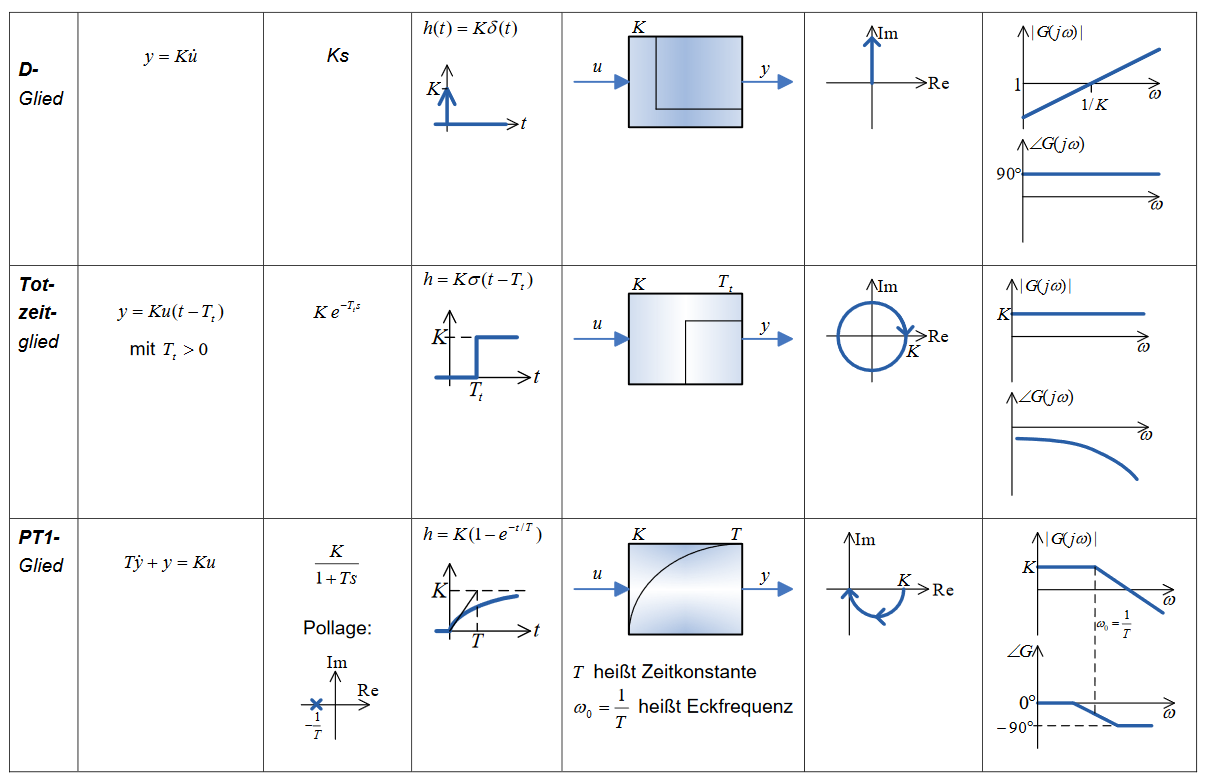
\includegraphics[width=1\columnwidth]{imgs/bb2_2b.png}
\end{figure}
\begin{figure}[H]
	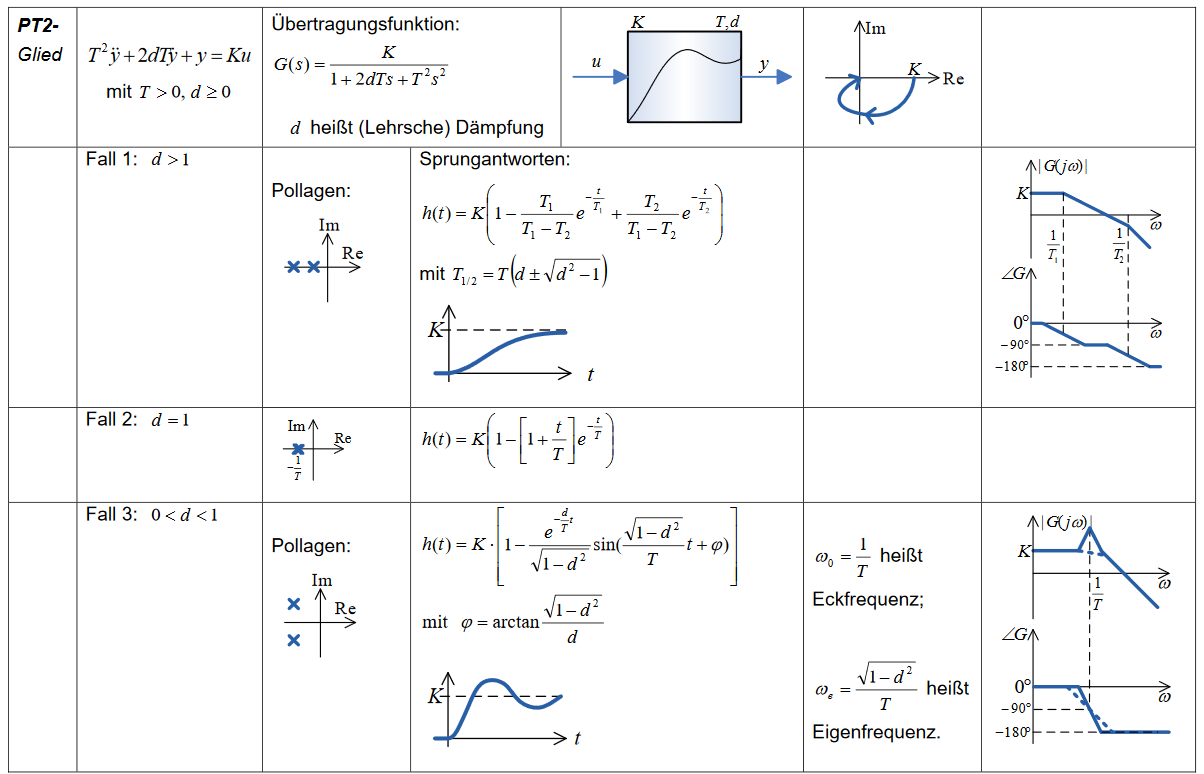
\includegraphics[width=1\columnwidth]{imgs/bb2_2c.png}
\end{figure}
\begin{figure}[H]
	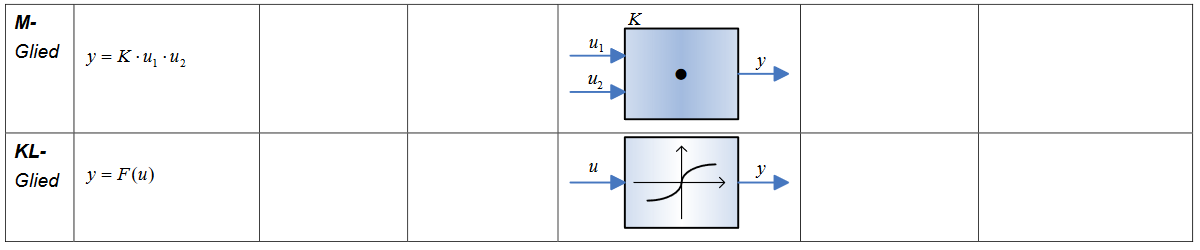
\includegraphics[width=1\columnwidth]{imgs/bb2_2d.png}
\end{figure}

Die Übertragungsglieder Summationsglied, Proportionalglied, Integrierglied, Differenzierglied und Totzeitglied sind linear.

\subsubsection{Sprungfunktion, Impulsfunktion}
\renewcommand{\arraystretch}{2}
$$
\begin{array}{ll}
	\text{Sprungfunktion} &	\sigma(t) = \begin{cases}
	0 & \text{für } t < 0 \\
	1 & \text{für } t ≥ 0
	\end{cases} \\
	\text{Impulsfunktion} & \delta(t) = \frac{d \sigma(t)}{dt} \\
	\text{Es gilt:} & \int_{-∞}^{∞} \delta(t) dt = 1 \\
	& \int_{-∞}^t \delta(t) dt = \sigma(t)
\end{array}
$$
\renewcommand{\arraystretch}{1.5}

\subsection{Lineare zeitinvariante Modelle (LZI-Modelle)}
\subsubsection*{Eigenschaften}
\begin{itemize}
	\item \textbf{Linearität:} Für $y(t) = \varphi(u(t))$ gilt:
	\begin{itemize}
		\item $\varphi(c_1 u_1(t) + c_2 u_2(t)) = c_1 \varphi(u_1(t)) + c_2 \varphi(u_2(t))$
	\end{itemize}
	\item \textbf{Zeitinvarianz:}
	\begin{itemize}
		\item $y(t) = \varphi(u(t))$ folgt $\varphi(u(t-T)) = y(t-T)$
	\end{itemize}
\end{itemize}

\subsubsection{Regelungsnormalform}
Das System $y^{(n)} + a_{n-1} y^{(n-1)} + \dots + a_1 \dot y + a_0 y = b_0 u$ \\
besitzt die Zustandsdarstellung
$$
	\dot x = \begin{bmatrix}
		0 & 1 & 0 & \dots & 0 \\
		0 & 0 & 1 & \ddots & \vdots \\
		\vdots & \vdots & \ddots & \ddots & 0 \\
		0 & 0 & \dots & 0 & 1 \\
		-a_0 & -a_1 & \dots & -a_{n-2} & -a_{n-1}
	\end{bmatrix} x + \vect{0 \\ \vdots \\ \vdots \\ 0 \\ b_0} u
$$
$$
	y = \vect{1 & 0 & \dots & 0} x
$$
Sie heißt Regelungsnormalform

\subsubsection{Regelungsnormalform mit Ableitungen von u}

Das System $y^{(n)} + a_{n-1} y^{(n-1)} + \dots + a_1 \dot y + a_0 y = b_{n-1} u^{n-1} + \dots + b_1 \dot u + b_0 u$ \\
besitzt die Zustandsdarstellung
$$
\dot x = \begin{bmatrix}
0 & 1 & 0 & \dots & 0 \\
0 & 0 & 1 & \ddots & \vdots \\
\vdots & \vdots & \ddots & \ddots & 0 \\
0 & 0 & \dots & 0 & 1 \\
-a_0 & -a_1 & \dots & -a_{n-2} & -a_{n-1}
\end{bmatrix} x + \vect{0 \\ \vdots \\ \vdots \\ 0 \\ 1} u
$$
$$
y = \vect{b_0 & b_1 & \dots & b_{n-1}} x
$$
Sie heißt Regelungsnormalform

\subsubsection{Beobachtungsnormalform}
Das System $y^{(n)} + a_{n-1} y^{(n-1)} + \dots + a_1 \dot y + a_0 y = b_{n-1} u^{n-1} + \dots + b_1 \dot u + b_0 u$ \\
besitzt die Zustandsdarstellung
$$
\dot x = \begin{bmatrix}
0 & 0 & \dots & 0 & -a_0 \\
1 & 0 & \ddots & 0 & -a_1 \\
0 & 1 & \ddots & 0 & -a_2\\
\vdots & \ddots & \ddots & 0 & \vdots \\
0 & \dots & 0 & 1 & -a_{n-1}
\end{bmatrix} x + \vect{b_0 \\ b_1 \\ b_2 \\ \vdots \\ b_{n-1}} u
$$
$$
y = \vect{0 & \dots & 0 & 1} x
$$
Sie heißt Beobachtungsnormalform

\subsection{Linearisierung im Arbeitspunkt}
\subsubsection{Ein Eingabeparameter} ~\\
Sei $y = F(u)$ eine Übertragungsfunktion. \\
Die linearisierte Funktion um den Arbeitspunkt $u_s$ ist berechnet als:
$$
	\Delta y = f(\Delta u, u_s) = \frac{\partial F(u)}{\partial u}\bigg|_{u = u_s} ⋅ \Delta u
$$
mit
$$
	\Delta y = y - y_s
$$
$$
	y_s = F(u_s)
$$
$$
	\Delta u = u - u_s
$$
Die um den Arbeitspunkt linearisierte Beziehung zwischen den absoluten Größen ist definiert als:
$$
	y_{lin} = f(u,u_s) = \Delta y + y_s \tab \text{(Ersetze $\Delta u$ durch $u - u_s$)}
$$

\subsubsection{Mehere Eingabeparameter} ~\\
Sei $y = F(u_1, \dots u_n)$ eine Übertragungsfunktion ($n \in \mathbb{N}$). \\
Die linearisierte Funktion um den Arbeitspunkt $(u_{1,s}, \dots, u_{n,s})$ wird wie folgt berechnet:
$$
\Delta y = f(\Delta u_1, \dots, \Delta u_n, u_{1,s}, \dots, u_{n,s}) = \frac{\partial F(u_1, \dots u_n)}{\partial u_1}\Bigg|_\textrm{AP} ⋅ \Delta u_1 + \dots + \frac{\partial F(u_1, \dots u_n)}{\partial u_n}\Bigg|_\textrm{AP} ⋅ \Delta u_n
$$
$$
	\textrm{AP} ≡ u_1 = u_{1,s}, \dots, u_n = u_{n,s}
$$
mit
$$
	\Delta y = y - y_s
$$
$$
	y_s = F(u_s)
$$
$$
	\Delta u_1 = u_1 - u_{1,s}, \dots, \Delta u_n = u_n - u_{n,s}
$$
Die um den Arbeitspunkt linearisierte Beziehung zwischen den absoluten Größen ist definiert als:
$$
y_{lin} = f(u_1, \dots, u_n, u_{1,s}, \dots, u_{n,s}) = \Delta y + y_s  \tab \text{(Ersetze $\Delta u_1$ durch $u_1 - u_{1,s}, \dots$)}
$$

\subsubsection{Regelungsnormalform}
Gegeben sei ein System in der Form $\dot x = Ax + ez + bu$, $y = c^T x$. \\
Die $n$ algebraischen Gleichungen seien definiert als: \\
$\begin{array}{l}
	f_1(x_1, \dots, x_n, z, u) = a_{11} x_1 + \dots + a_{1n} x_n + e_1 z + b_1 u \\
	\tab \vdots \\
	f_n(x_1, \dots, x_n, z, u) = a_{n1} x_1 + \dots + a_{nn} x_n + e_n z + b_n u
\end{array}$ \\
Die Ausgangsgröße sei definiert als:
$g(x_1, \dots, x_n) = y = c_1 x_1 + \dots + c_n x_n$ \\
Das linearisierte Modell wird wie folgt berechnet:
$$
	\Delta \dot x(t) = A_l \Delta x(t) + e_l \Delta z(t) + b_l \Delta u(t)
$$
$$
	\Delta y(t) = c_l^T \Delta x(t)
$$
$$
	A_l = \left. \begin{bmatrix}
		\frac{\partial f_1}{\partial x_1} & \dots & \frac{\partial f_1}{\partial x_n} \\
		\vdots & \ddots & \vdots \\
		\frac{\partial f_n}{\partial x_1} & \dots & \frac{\partial f_n}{\partial x_n} \\
	\end{bmatrix}\right |_\textrm{AP}
$$
$$
	e_l = \left.\vect{\frac{\partial f_1}{\partial z} \\ \vdots \\ \frac{\partial f_n}{\partial z}}\right |_\textrm{AP}
$$
$$
	b_l = \left.\vect{\frac{\partial f_1}{\partial u} \\ \vdots \\ \frac{\partial f_n}{\partial u}}\right |_\textrm{AP}
$$
$$
	c_l^T = \left.\vect{\frac{\partial g}{\partial x_1} & \dots & \frac{\partial g}{\partial x_n}}\right |_\textrm{AP}
$$

\section{Laplace-Transformation}
\begin{figure}[H]
	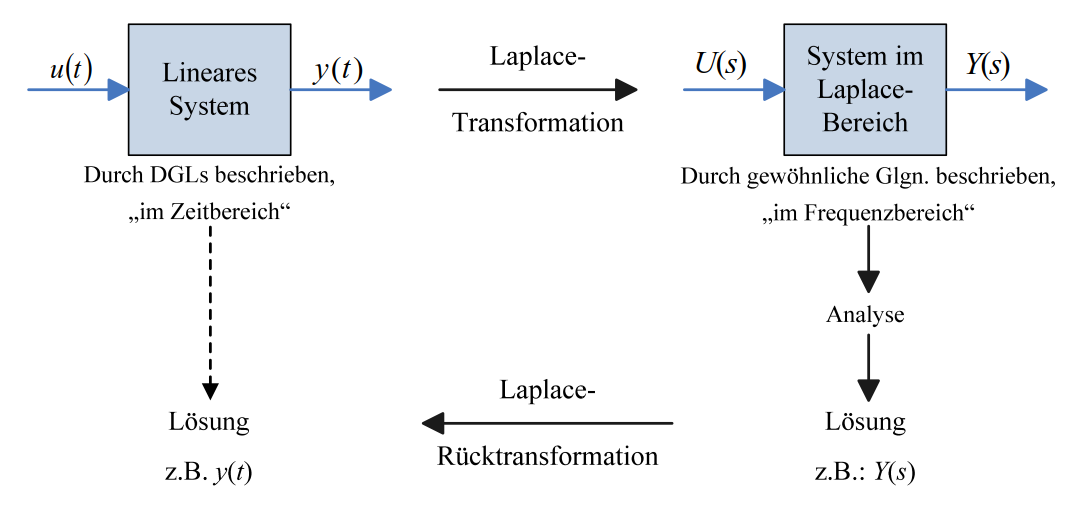
\includegraphics[width=0.8\columnwidth]{imgs/laplace.png}
\end{figure}

\subsection{Definition}
Sei $f(t)$ eine Zeitfunktion mit $f(t) = 0$ für $t < 0$. \\
Die Laplace-Transformierte dieser Zeitfunktion ist definiert als:
$$
	F(s) = \mathcal{L}\{f(t)\} = \int_0^{∞} f(t) e^{-st} dt
$$
wobei
$s = \delta + j \omega$ \\

Die Korrespondenz wird wie folgt dargestellt:
$$
	f(t) ~\laplace ~F(s)
$$

\subsection{Rücktransformation}
Sei $F(s)$ die Laplace-Transformierte zu $f(t)$. \\
Die Rücktransformation ist definiert als:
$$
	f(t) = \mathcal{L}^{-1}\{F(s)\} = \frac 1 {2\pi j} \int_{c - j ∞}^{c + j∞} F(s) e^{st} ds
$$
mit $c$ in der Konvergenzhalbebene.

\pagebreak
\begin{multicols}{2}
\subsection{Korrespondenztabelle}

\begin{tabularx}{\columnwidth}{|X|X|}
	\hline
	$f(t)$ & $F(s)$ \\
	\hline
	\hline
	$\delta(t)$ (Dirac-Impuls)& 1 \\
	\hline
	$\delta(t - t_0)$ & $e^{-t_0 s}$ \\
	\hline
	$\sigma(t)$ (Einheitssprung) & $\frac 1 s$ \\
	\hline
	$\sigma(t - t_0)$ & $\frac{e^{-t_0 s}}{s}$ \\
	\hline
	$t$ & $\frac{1}{s^2}$ \\
	\hline
	$\frac{t^n}{n!}, n \in \mathbb{N}_0$ & $\frac{1}{s^{n + 1}}$ \\
	\hline
	$e^{\alpha t}$ & $\frac{1}{s - \alpha}$ \\
	\hline
	$\frac 1 T e^{-\frac t T}$ & $\frac{1}{1 + Ts}$ \\
	\hline
	$te^{\alpha t}$ & $\frac{1}{(s - \alpha)^2}$ \\
	\hline
	$\frac{t}{T^2} e^{- \frac t T}$ & $\frac{1}{(1 + Ts)^2}$ \\
	\hline
\end{tabularx}
\begin{tabularx}{\columnwidth}{|X|X|}
	$\frac{t^n}{n!}e^{\alpha t}$ & $\frac{1}{(s - \alpha)^{n + 1}}$ \\
	\hline
	$1 - e^{\alpha t}$ & $\frac{-\alpha}{s(s - \alpha)}$ \\
	\hline
	$1 - e^{-\frac{t}{T}}$ & $\frac{1}{s(1 + Ts)}$ \\
	\hline
	$\sin \omega t$ & $\frac{\omega}{s^2 + \omega^2}$ \\
	\hline
	$\cos \omega t$ & $\frac{s}{s^2 + \omega^2}$ \\
	\hline
	$e^{-\delta t}\sin \omega t$ & $\frac{\omega}{(s + \delta)^2 + \omega^2}$ \\
	\hline
	$e^{-\delta t}\cos \omega t$ & $\frac{s + \delta}{(s + \delta)^2 + \omega^2}$ \\
	\hline
	$t \sin \omega t$ & $\frac{2 \omega s}{(s^2 + \omega^2)^2}$ \\
	\hline
	$t \cos \omega t$ & $\frac{s^2 - \omega^2}{(s^2 + \omega^2)^2}$ \\
	\hline	
\end{tabularx} \\
\\

wobei \\
$f(t) = 0$ für $t < 0$, \\
$T > 0, t_0 > 0, \omega > 0$ reell, \\
$\delta$ beliebig reell und \\
$\alpha$ beliebig komplex.
\end{multicols}

\subsection{Eigenschaften der Laplace-Transformation}
\begin{tabularx}{\columnwidth}{|X|X|X|}
	\hline
	Eigenschaft & Operation im Zeitbereich & Operation im Bildbereich \\
	\hline
	\hline
	Linearität & $c_1f_1(t) + c_2f_2(t)$ & $c_1 F_1(s) + c_2 F_2(s)$ \\
	\hline
	Differenziation & $\dot f(t)$ & $sF(s) - f(0)$ \\
	& $f^{(n)}(t)$ & $s^n F(s) - s^{n - 1} f(0) - \dots - f^{(n-1)}(0)$ \\
	\hline
	Integration & $\int_0^t f(\tau) ~d\tau$ & $\frac 1 s F(s)$ \\
	\hline
	Dämpfung & $f(t) ⋅ e^{\alpha t}$ & $F(s-\alpha)$ \\
	\hline
	Faltung & $f_1(t) * f_2(t)$ & $F_1(s) ⋅ F_2(s)$ \\
	\hline
	Zeitverschiebung & $f(t - t_0), t_0 > 0$ & $e^{-t_0 s}F(s)$ \\
	\hline
	Diffenrentiation der Bildfunktion & $(-1)^n t^n f(t)$ & $F^{(n)}(s), n \in \mathbb{N}$ \\
	\hline
	Skalierung der Zeitachse & $f(\alpha t), \alpha > 0$ & $\frac 1 \alpha F(\frac s \alpha)$ \\
	\hline
	Anfangswertsatz & \multicolumn{2}{X|}{$\lim_{t → +0} f(t) = \lim_{s → ∞} s F(s)$, sofern $\lim_{t → +0} f(t)$ existiert} \\
	\hline
	Endwertsatz & \multicolumn{2}{X|}{$\lim_{t → ∞} f(t) = \lim_{s → 0} sF(s)$, sofern $\lim_{t → ∞} f(t)$ existiert} \\
	\hline
\end{tabularx}

\subsection{Lösung linearer zeitinvarianter Differentialgleichungen mittels Laplace-Transformation}
Sei $a_ny^{(n)} + \dots + a_1 \dot y + a_0 y = b_m u^{(m)} + \dots + b_1 \dot u + b u$ mit $m ≤ n$ und $a_n ≠ 0$ die systembeschreibende Differentialgleichung.
Die Lösung dieser DGL erfolgt durch die folgenden 5 Schritte:
\begin{enumerate}
	\item Transformation der DGL in den Bildbereich mittels Laplace-Transformation
	\item Auflösen nach $Y(s)$. Sind alle Anfangswerte gleich null, resultiert: \\
	$Y(s) = \frac{b_ms^m + \dots + b_1s + b_0}{a_ns^n + \dots + a_1s + a_0} U(s) ≡ Y(s) = G(s) ⋅ U(s)$
	\item Einsetzen von $U(s) ~\Laplace ~u(t)$ in $Y(s) = G(s) ⋅ U(s)$
	\item Durchführung einer Partialbruchzerlegung von $Y(s)$
	\item Rücktransformation in den Zeitbereich $y(t) ~\laplace ~Y(s)$
\end{enumerate}

\subsubsection{Darstellungsformen von G(s)}
\label{darstell_gs}
$G(s)$ kann in folgenden Formen dargestellt werden: \\
\begin{tabular}{lll}
	Polynomform: & $G(s) = \frac{b_ms^m + \dots + b_1s + b_0}{a_ns^n + \dots + a_1s + a_0}$ \\
	Linearfaktorform: & $G(s) = Q \frac{(s - q_1) ⋅ \dots ⋅ (s - q_m)}{(s - p_1)⋅ \dots ⋅ (s - p_n)}$ & mit $Q = \frac{b_m}{a_n}$ \\
	Zeitkonstantenform: & $G(s) = K \frac{(1 + \bar{T}_1 s) ⋅ \dots ⋅ (1 + \bar{T}_m s)}{(1 + T_1s) ⋅ \dots ⋅ (1 + T_n s)}$ & mit $\bar{T}_i = - \frac 1 {q_i}$, $T_i = -\frac 1 {p_i}$, $K = \frac{b_0}{a_0}$ \\
	Partialbruchform: & $G(s) = r_0 + \frac{r_1}{s - p_1} + \dots + \frac{r_n}{s - p_n}$
\end{tabular}

\subsubsection{Komplexe Übertragungsfunktion}
Sei $Y(s) = G(s)U(s)$ eine systembeschreibende Differentialgleichung im Bildbereich. \\
$G(s) = \frac{Y(s)}{U(s)}$ heißt komplexe Übertragungsfunktion. \\
Komplexe Übertragungsfunktionen der in Sektion \ref{darstell_gs} genannten Darstellungsformen heißen rationale Übertragungsfunktionen. Die zugehörigen Übertragungsglieder heißen rationale Übertragungsglieder, kurz R-Glieder.

\subsection{Sprungantworten des PT2-Gliedes}
Die Pole von der komplexen Übertragungsfunktion $G(s)$ eines PT2-Gliedes werden wie folgt berechnet:
$$
	p_{1/2} = \frac 1 T (-d \pm \sqrt{d^2 - 1})
$$
Es folgt: \\
\begin{tabular}{llll}
	Fall 1: & $d > 1$, & $p_{1/2} \in \mathbb{R}^-$, & aperiodischer Fall \\
	Fall 2: & $d = 1$, & $p_1 = p_2, p_{1/2} \in \mathbb{R}^-$, & aperiodischer Grenzfall \\
	Fall 3: & $0 < d < 1$, & $p_{1/2} \in \mathbb{C}, \Re(p_{1/2}) < 0$, & unterkritisch/periodisch gedämpfter Fall \\
	Fall 4: & $d = 0$, & $p_{1/2} \in \mathbb{C} \backslash \mathbb{R}$, & ungedämpfter Fall
\end{tabular}

\subsection{Lösung der Zustandsgleichung mittels Laplace-Transformation}
Sei ein LZI-System gegeben mit $\dot x = Ax + bu$ und $y = c^T x$. \\
Die Zustandsgleichungen im Bildbereich sind:
$$
	X(s) = (sI-A)^{-1} b U(s) + (sI-A)^{-1} x(0) ~\Laplace ~x(t)
$$
$$
	Y(s) = c^T(sI-A)^{-1} b U(s) + c^T (sI - A)^{-1} x(0) ~\Laplace ~y(t)
$$
Die komplexe Übertragungsfunktion $G(s)$ ist:
$$
	G(s) = c^T(sI - A)^{-1} b = \frac{c^T(\textrm{Adjunkte}(sI-A))b}{\det(sI-A)} = \frac{Z(s)}{N(s)}
$$
%TODO add G(s) (geschweifte Klammer unten ...)

\subsubsection{Polstellen}
Jeder Pol von $G(s)$ ist Eigenwert von $A$. Ein Eigenwert von $A$ ist genau dann Pol von $G(s)$, wenn er sich nicht herauskürzt, d.h. nicht gleichzeitig Nullstelle von $Z(s)$ ist.

\subsubsection{Zustandsgleichung mit Störgröße}
Seien die Zustandsgleichungen des LZI-Systems gegeben durch $\dot x = Ax + ez + bu$ und $y = c^T x$. \\
Die Zustandsgleichung im Bildbereich ist:
$$
	Y(s) = G(s) U(s) + G_z(s) Z(s)
$$
und die Störübertragungsfunktion ist
$$
	G_z(s) = c^T(sI-A)^{-1}e
$$

\subsection{Lösung der Zustandsgleichungen im Zeitbereich}
Sei ein LZI-System gegeben mit $\dot x = Ax + bu$ und $y = c^T x$. \\
Die Lösungen dieser Gleichungen sind:
$$
	x(t) = \int_0^t e^{A(t-\tau)} b u(\tau) ~d\tau + e^{At} x(0)
$$
$$
	y(t) = \int_0^t c^T e^{A(t-\tau)} bu(\tau) ~d\tau + c^T e^{At} x(0)
$$
wobei
$$
	e^{At} = I + A\frac{t}{1!} + A^2 \frac{t^2}{2!} + \dots
$$

\subsubsection{Transitionsmatrix}
Die Matrix $e^{At}$ heißt Überführungs- bzw. Transitionsmatrix.
Sie hat folgende Eigenschaften.
$$
	e^{At} ⋅ e^{A\tau} = e^{A(t + \tau)}
$$
$$
	e^{-At} ⋅ e^{At} = e^0 = I
$$
$$	
	\frac{d e^{At}}{dt} = Ae^{At} = e^{At} A
$$

\section{Analyse dynamischer Systeme}
\subsection{Systemantworten}
\subsubsection{Impulsantwort}
\begin{figure}[H]
	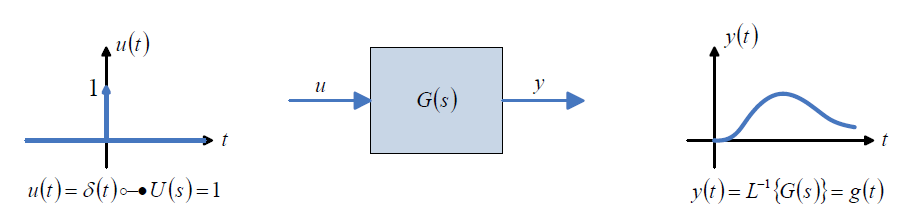
\includegraphics[width = \columnwidth]{imgs/impulsantwort.png}
\end{figure}
Sei $Y(s) = G(s) U(s)$ ein lineares zeitinvariantes System mit der komplexen Übertragungsfunktion $G(s)$. \\
Die Impulsantwort dieses Systems ist:
$$
	Y(s) = G(s) ~\Laplace ~g(t)
$$
mit $u(t) = \delta(t) ~\laplace ~U(s) = 1$,

\paragraph{Eigenschaften} ~\\
Sei $G(s)$ ein R-Glied in der Form: $G(s) = \sum_{i = 1}^n \frac{r_i}{s - p_i} ~\Laplace ~g(t) = \sum_{i = 1}^n r_i e^{p_i t}$ \\
und sei $p_i$ der zugehörige $i$-te Pol. \\
Für den Charakter des zugehörigen Zeitsignals folgt: \\
\begin{tabularx}\columnwidth{Xlll}
	einfacher negativ reeller Pol $p_i$, & $p_i \in \mathbb{R}^-$: & abklingende $e$-Funktion, & $r_ie^{p_it}$ \\
	einfacher Pol in null, & $p_i = 0$: & konstanter Anteil, & $r_i$\\
	einfacher positiv reeller Pol $p_i$, & $p_i \in \mathbb{R}^+$: & aufklingende $e$-Funktion, & $r_ie^{p_it}$ \\	
	einfaches, in der linken Halbebene gelegenes konjugiert komplexes Polpaar, & $p_{1/2} = -\delta \pm j \omega \in \mathbb{C}, \Re(p_{1/2}) < 0$: & abklingende Schwingung, & $e^{-\delta t} \sin(\omega t + \phi)$ \\
	einfaches, auf der imaginären Achse gelegenes komplexes Polpaar, & $p_{1/2} = \pm j \omega \in \mathbb{C} \backslash \mathbb{R}$: & harmonische Dauerschwingung, & $\sin(\omega t + \varphi)$ \\
	einfaches, in der rechten Halbebene gelegenes konjugiert komplexes Polpaar, & $p_{1/2} = +\delta \pm j \omega \in \mathbb{C}, \Re(p_{1/2}) > 0$: & aufklingende Schwingung, & $e^{\delta t} \sin(\omega t + \varphi)$ \\
\end{tabularx}
\begin{figure}[H]
	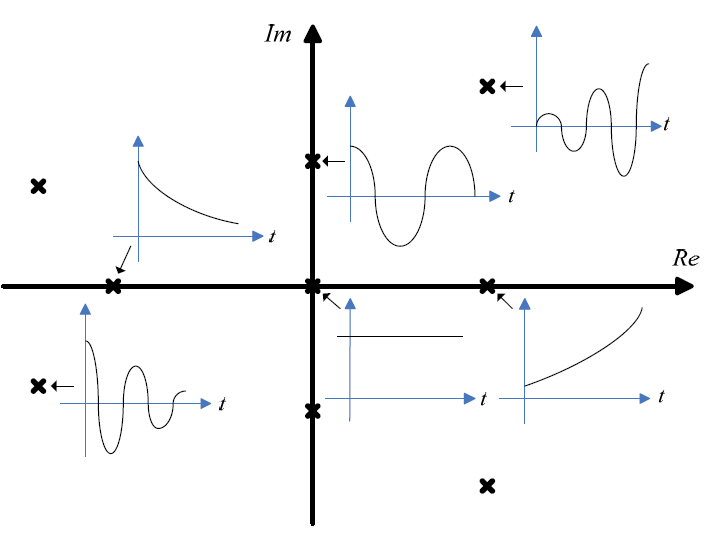
\includegraphics[width = 0.7\columnwidth]{imgs/polstellen.png}
\end{figure}

\paragraph{Impulsantwort bei Zustandsdarstellung} ~\\
Sei ein LZI-System gegeben mit $\dot x = Ax + bu$ und $y = c^T x$. \\
Die Impulsantwort dieses Systems ist:
$$
	g(t) = c^T e^{At} b \sigma(t)
$$
wobei $x(0) = 0$

\subsubsection{Sprungantwort}
\begin{figure}[H]
	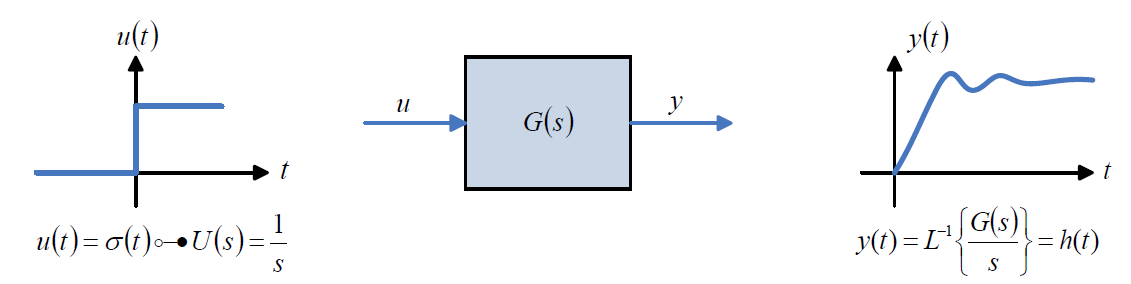
\includegraphics[width = \columnwidth]{imgs/sprungantwort.png}
\end{figure}
Sei $Y(s) = G(s) U(s)$ ein lineares zeitinvariantes System mit der komplexen Übertragungsfunktion $G(s)$. \\
Die Sprungantwort dieses Systems ist:
$$
	Y(s) = \frac{G(s)} s = H(s) ~\Laplace ~h(t) = \int_0^t g(\tau) d\tau
$$
mit $u(t) = \sigma(t) ~\laplace ~U(s) = 1/s$,

\subsubsection{Systemantwort mittels Faltung}
Sei ein lineares zeitinvariantes System gegeben mit Eingangssignal $u(t)$, Ausgangssignal $y(t)$ und der Übertragungsfunktion $g(t)$. \\
Das Ein-Ausgangsverhalten dieses Systems lässt beschreiben durch:
$$
	y(t) = g(t) * u(t)
$$
wobei $g(t) * u(t) = \int_0^t g(t - \tau) u(\tau) d \tau$ die Faltungsoperation ist.

\subsubsection{Anfangswertsatz der Laplace-Transformation}
Sei $y(t)$ eine Zeitfunktion sowie $Y(s)$ deren Laplace-Transformierte. \\
Es gilt:
$$
	y(t → 0^+) = \lim_{s → ∞} [sY(s)], \tab \text{sofern $y(t → 0^+)$ existiert}
$$

Für die Sprungantwort gilt:
$$
	h(t → 0^+) = G(∞)
$$

\subsubsection{Endwertsatz der Laplace-Transformation}
Sei $y(t)$ eine Zeitfunktion sowie $Y(s)$ deren Laplace-Transformierte. \\
Es gilt:
$$
y(t → ∞) = \lim_{s → 0} [sY(s)], \tab \text{sofern $y(t → ∞)$ existiert}
$$

Für die Sprungantwort gilt:
$$
h(t → ∞) = G(0), \tab \text{sofern alle Pole von $G(s)$ links der $j$-Achse sind}
$$

\subsection{Stabilität}
\subsubsection{Sprungantwortstabilität}
Ein lineares zeitinvariantes System ist sprungantwortstabil, falls
$$
	h(t → ∞) = \int_0^∞ g(\tau) d \tau  = c < ∞
$$
wobei $h(t) = \int_0^t g(\tau) d \tau$ die Sprungantwort des Systems ist. \\

Ein rationales Übertragungsglied (R-Glied) ist genau dann sprungantwortstabil, wenn alle Pole der Übertragungsfunktion $G(s)$ in der linken komplexen Halbebene liegen.

\subsubsection{Übertragungsstabilität, BIBO-Stabilität}
\begin{itemize}
	\item Ein dynamisches System heißt übertragungsstabil, wenn es auf jedes beschränkte Eingangssignal mit einem beschränkten Ausgangssignal antwortet. 
	\item Andere Bezeichnungen sind: äußere Stabilität, Ein-/Ausgangsstabilität, BIBO (Bounded Input Bounded Ouput) Stabilität
	\item Sprungantwortstabilität $\iff$ Übertragungsstabilität
\end{itemize}

\subsubsection{Asymptotische Stabilität}
Sei ein LZI-System gegeben mit $\dot x = Ax + bu$ und $y = c^T x$
\begin{itemize}
	\item Das Zustandsraummodell heißt asymptotisch stabil, wenn $x(t) → 0$ für $u(t) = 0$ und beliebige Anfangswerte $x(0)$
	\item Das Zustandsraummodell ist genau dann asymptotisch stabil, wenn alle Eigenwerte der Matrix $A$ in der linken komplexen Halbebene liegen.
	\item Andere Bezeichnungen sind: Zustandsstabilität, innere Stabilität
	\item Asymptotische Stabilität $\implies$ Übertragungsstabilität
	\item Übertragungsstabilität $\implies$ Asymptotische Stabilität, falls \\ das Zählerpolynom der Übertragungsfunktion $G(s)$ keine der Nennernullstellen kürzt und der Nennergrad von $G(s)$ tatsächlich die Ordnung des Zustandsraummodells widerspiegelt.
\end{itemize}

\paragraph{Asymptotisch stabiles R-Glied} ~\\
Sei $G(s) = \frac{b_m s^m + \dots + b_0}{a_n s^n + \dots + a_0}, n ≥ m, a_n ≠ 0$ die komplexe Übertragungsfunktion eines R-Gliedes und \\
sei $a_n y^{(n)} + \dots + a_1 \dot y + a_0 y = b_m u^{(m)} + \dots + b_1 \dot u + b_0 u$ das zugehörige Zustandsraummodell der Ordnung $n$. \\
Das Zustandsraummodell der Ordnung $n$ ist genau dann asymptotisch stabil, wenn alle $n$ Systempole, also die Lösungen der charakteristischen Gleichung $a_n s^n + \dots + a_1 s + a_0 = 0$ in der linken komplexen Halbebene liegen.

\subsection{Pole, Nullstellen und Modellreduktion}
\subsubsection{Dominierende Pole}
\begin{figure}[H]
	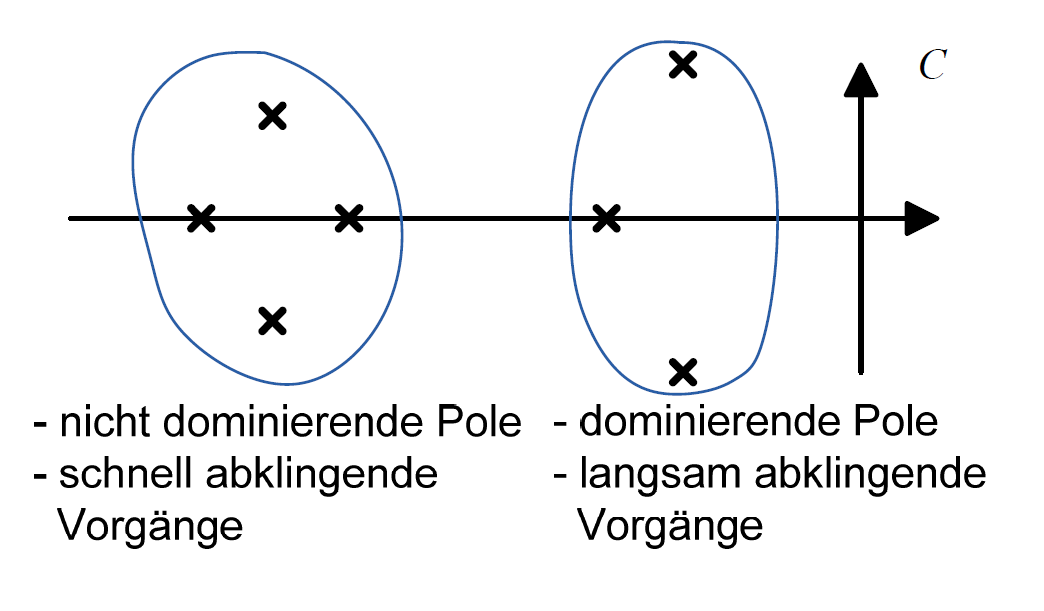
\includegraphics[width = 0.5\columnwidth]{imgs/pole_dominanz.png}
\end{figure}
\begin{itemize}
	\item näher an der imaginären Achse (links) liegende Pole sind dominante Pole → langsam abklingende $e$-Funktion
	\item weiter von der imaginären Achse entfernt (links) liegende Pole sind nicht-dominante Pole → schnell abklingende $e$-Funktion
\end{itemize}

\subsubsection{Nullstelleneffekte}
\paragraph{Blockiereigenschaft einer Nullstelle} ~\\
Sei $G(s)$ eine komplexe Übertragungsfunktion mit der Nullstelle $\eta$. \\
Die spezielle Anregung $u(t) = u_0 e^{\eta t}$ bewirkt in der Systemantwort $y(t)$ keinen Anteil $re^{\eta t}$, \\
d.h. die Nullstelle blockiert.

\paragraph{Wirkung der Nullstellenlage auf den Verlauf der Sprungantwort} ~\\
\begin{itemize}
	\item In der linken Halbebene gelegene Nullstellen
	\begin{itemize}
		\item links von den dominanten Polen: geringe Wirkung
		\item rechts von den dominanten Polen: Überschwingen oder sonstigen "Verbeulen" der Sprungantwort
	\end{itemize}
	\item In der rechten Halbebene gelegene Nullstellen
	\begin{itemize}
		\item schwieriger zu regeln
		\item z.B. Allpassglied: $G(s) = - \frac{(Ts - 1)}{(Ts + 1)}$, Sprungantwort beginnt bei $-1$ und endet bei $1$ für alle $T > 0$
	\end{itemize}
\end{itemize}

\subsubsection{Modellreduktion}
\textbf{Ziel:} \\
Entferne nicht dominierende Pole aus der komplexen Übertragungsfunktion und gelange so zu einem reduzierten Modell. \\

\textbf{Verfahren:} \\
Aus $G(s) = \sum_{v = 1}^n \frac{r_v}{s - p_v}$ werden diejenigen Summanden ersatzlos gestrichen, deren Dominanzmaß $D_v = |\frac{r_v}{p_v}|$ vergleichsweise klein ist. \\
Rechts oder auf der imaginären Achse gelegene Pole werden nicht gestrichen.

\subsection{Approximation des Totzeitgliedes}
Sei $G(s) = e^{-T_t s}$ die komplexe Übertragunsfunktion eines Totzeitgliedes. \\
Das Totzeitglied kann durch eine rationale Übertragungsfunktion angenähert und ersetzt werden. \\
Je höher die Ordnung $n$ ist, desto genauer ist die Approximation.

\subsubsection{Approximation durch ein PTn-Glied}
Wird für die Annäherung ein PT$n$-Glied angesetzt, so folgt:
$$
	G(s) \approx \frac{1}{(1 + \frac{T_t}{n}s)^n}
$$

\subsubsection{Padé-Approximation}
Wird für die Annäherung eine Padé-Approximation vorgenommen, so wird ein allgemeines rationales Übertragungsglied angesetzt und die Zähler- und Nennerkoeffizienten so gewählt, dass die zugehörige Taylorreihe um $s = 0$ in möglichst vielen Gliedern mit der Taylorreihe von $e^{-T_t s}$ übereinstimmt. \\

\textbf{Padé-Approximationen des Totzeitgliedes:} \\
\renewcommand{\arraystretch}{2}
$\begin{array}{l|c|c}
	\text{Ordnung} & \text{Padé-Approximation mit Zählergrad }n & \text{Padé-Approximation mit Zählergrad }n-1 \\
	\hline
	n = 1 & \frac{1 - \frac 1 2 T_t s}{1 + \frac 1 2 T_t s} & \frac{1}{1 + T_t s} \\
	n = 2 & \frac{1 - \frac 1 2 T_t s + \frac 1 {12} T_t^2 s^2}{1 + \frac 1 2 T_t s + \frac 1 {12} T_t^2 s^2} & \frac{1 - \frac 1 3 T_t s}{1 + \frac 2 3 T_t s + \frac 1 6 T_t^2 s^2} \\
	n = 3 & \frac{1 - \frac 1 2 T_t s + \frac 1 {10} T_t^2 s^2 - \frac 1 {120} T_t^3 s^3}{1 + \frac 1 2 T_t s + \frac 1 {10} T_t^2 s^2 + \frac 1 {120} T_t^3 s^3} & \frac{1 - \frac 2 5 T_t s + \frac 1 {20} T_t^2 s^2}{1 + \frac 3 5 T_t s + \frac 3 {20} T_t^2 s^2 + \frac 1 {60} T_t^3 s^3} \\	
\end{array}$
\renewcommand{\arraystretch}{1.5}

\subsection{Modellidentifikation im Zeitbereich}
Sei die Sprungantwort eines Systems als $t-\Delta y(t)$ Diagramm gegeben. \\

\textbf{Annäherung durch Totzeitglied und PT1-Glied:} \\
\begin{figure}[H]
	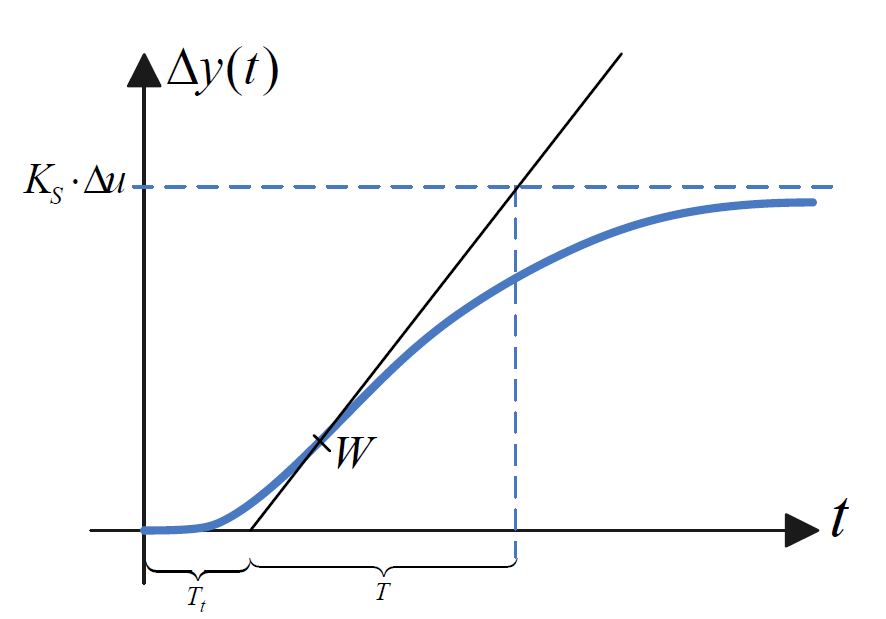
\includegraphics[width = 0.4\columnwidth]{imgs/modellidentifikation_1.png}
\end{figure}
Der Verlauf kann durch ein Totzeitglied und ein nachgeschaltetes PT1-Glied angenähert werden.
\begin{enumerate}
	\item Lege zeichnerisch die Wendetangente an die Kurve und bestimme die Totzeit $T_t$ und die Zeitkonstante $T$ des PT1-Gliedes wie im Bild angegeben.
	\item $G(s) = \frac{K_s}{1 + Ts} e^{-T_ts}$
\end{enumerate}

\textbf{Annäherung durch ein PTn-Glied:} \\
\begin{figure}[H]
	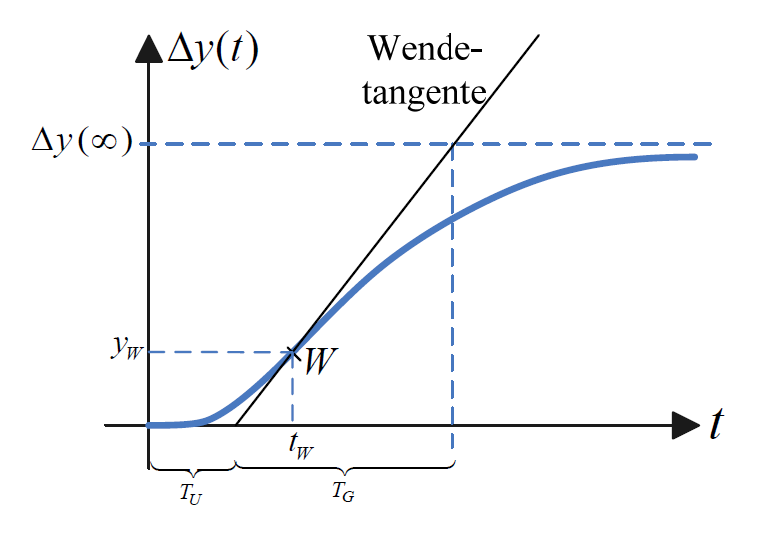
\includegraphics[width = 0.4\columnwidth]{imgs/modellidentifikation_2.png}
\end{figure}
Der Verlauf kann durch ein PT$n$-Glied angenähert werden.
\begin{enumerate}
	\item Lege zeichnerisch die Wendetangente an die Kurve und bestimme die Verzugszeit $T_U$, die Ausgleichszeit $T_G$, sowie $t_W$ und $y_W$ wie im Bild angegeben.
	\item $K = \frac{\Delta y(∞)}{\Delta u}$, wobei $\Delta u$ die Höhe des sprungförmigen Eingangssignal bezeichnet
	\item Die Ordnung $n$ wird aus der Tabelle abgelesen, anhand von $\frac{T_U}{T_G}$ oder $\frac{y_w}{\Delta y(∞)}$
	\item Mithilfe der Werte $T_U, T_G, t_W$ und $n$ und der Tabelle bestimmt man drei Werte für $T$. Der Mittelwert wird schließlich verwendet.	
	\item $G(s) = \frac{K}{(1 + Ts)^n}$
\end{enumerate}

Tabelle: \\
\begin{tabular}{|c|c|c|c|c|c|}
	\hline
	$n$ & $\frac{T_U}{T_G}$ & $\frac{y_W}{\Delta y(∞)}$ & $\frac{t_W}{T}$ & $\frac{T_G}{T}$ & $\frac{T_U}{T}$ \\
	\hline
	1 & 0 & 0 & 0 & 1 & 0 \\
	\hline
	2 & 0,104 & 0,264 & 1 & 2,718 & 0,282 \\
	\hline
	3 & 0,218 & 0,323 & 2 & 3,695 & 0,805 \\
	\hline
	4 & 0,319 & 0,353 & 3 & 4,463 & 1,425 \\
	\hline
	5 & 0,410 & 0,371 & 4 & 5,119 & 2,100 \\
	\hline
	6 & 0,493 & 0,384 & 5 & 5,699 & 2,811 \\
	\hline
	7 & 0,570 & 0,394 & 6 & 6,226 & 3,549 \\
	\hline
	8 & 0,642 & 0,401 & 7 & 6,711 & 4,307 \\
	\hline
	9 & 0,709 & 0,407 & 8 & 7,164 & 5,081 \\
	\hline
	10 & 0,773 & 0,413 & 9 & 7,590 & 5,869 \\
	\hline
\end{tabular}

\subsection{Frequenzgang}
\subsubsection{Systemantwort auf harmonische Anregung}
Sei $Y(s) = G(s)U(s)$ die beschreibende Gleichung eines R-Gliedes, welches mit $u(t) = \sin(\omega t)$ angeregt wird. \\
Die Antwort diese R-Gliedes ist:
$$
	y(t) = y_D(t) + y_G(t)
$$
mit dem Dauerschwingungsanteil
$$
	y_D(t) = |G(j\omega)| \sin(\omega t + \angle G(j \omega))
$$ \\

Ist das System $G(s)$ stabil, so gilt für große $t$:
$$
	y(t) = y_D(t)
$$

\textbf{Größen:} \\
\begin{tabular}{ll}
	Frequenzgang des Systems: & $G(j \omega)$ \\
	Betrag des Frequenzgangs: & $|G(j \omega)|$ \\
	Phase des Frequenzgangs: & $\angle G(j \omega) = \arctan(-\omega T)$
\end{tabular} \\

wobei
$$
	G(j \omega) = |G(j \omega)| e^{j \angle G(j \omega)}
$$

\subsubsection{Frequenzgangortskurve und Bode-Diagramm}
Sei $Y(s) = G(s)U(s)$ die beschreibende Gleichung eines Systems. \\

\textbf{Frequenzgangortskurve:} \\
Die Frequenzgangortskurve ist die Ortskurve $G(j \omega)$ für $0 ≤ \omega < ∞$ in der komplexen Zahlenebene. \\
Die Pfeilspitze zeigt in Richtung wachsender Frequenz $\omega$. \\

\textbf{Amplitudengang:} \\
Der Amplitudengang/Betragskennlinie ist $|G(j \omega)|$ für $0 < \omega < ∞$. \\
Die $|G(j \omega)|$-Achse wird in Dezibel (dB) skaliert, mit $|G|_{dB} = 20\log|G|$. \\

\textbf{Phasengang:} \\
Der Phasengang/Phasenkennlinie ist $\angle G(j \omega)$ für $0 < \omega < ∞$. \\
Die $\angle G(j \omega)$-Achse wird in Grad angegeben; die $\omega$-Achse wird logarithmisch aufgetragen. \\

\textbf{Bode-Diagramm:} \\
Betrags- und Phasenkennlinie zusammen heißen Bode-Diagramm bzw. Frequenzkennlinien des Systems $G(s)$.

%TODO Beispieldiagramme

\subsubsection{Konstruktion von Bode-Diagramm}
Sei die komplexe Übertragungsfunktion eines R-Gliedes als Produkt einfacher Glieder gegeben, d.h.:
$$
	G(s) = K ⋅ \frac{(s-q_1) ⋅ \dots ⋅ (s - q_m)}{(s - p_1) ⋅ \dots ⋅ (s - p_n)} = K ⋅ (s - q_1) ⋅ \dots ⋅ (s - q_m) ⋅ \frac{1}{s - p_1} ⋅ \dots ⋅ \frac{1}{s - p_n} = K ⋅ G_1 ⋅ \dots ⋅ G_m ⋅ G_{m+1} ⋅ \dots ⋅ G_{n + m}
$$

Die Betragskennlinie ist:
$$
	|G(j \omega)|_{dB} = 20 \log |G_1| + \dots + 20 \log |G_{n + m}
$$

Die Phasenkennlinie ist:
$$
	\angle G(j \omega) = \angle G_1 + \dots + \angle G_{n + m}
$$

\section{Regelkreis und Stabilität}
\subsection{Umformung von Blockschaltbildern}
Blockschaltbilder lassen sich gemäß folgender Regeln umformen, wobei jeweils die linke und rechte Darstellung äquivalent sind. \\

\textbf{Serienschaltung:}
\begin{figure}[H]
	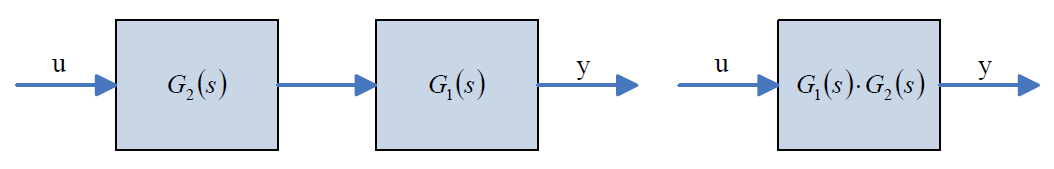
\includegraphics[width = \columnwidth]{imgs/serienschaltung.png}
\end{figure}
$$
	Y(s) = G_1(s) ⋅ (G_2(s) ⋅ U(s)) = (G_1(s) ⋅ G_2(s)) ⋅ U(s)
$$ \\

\textbf{Parallelschaltung:}
\begin{figure}[H]
	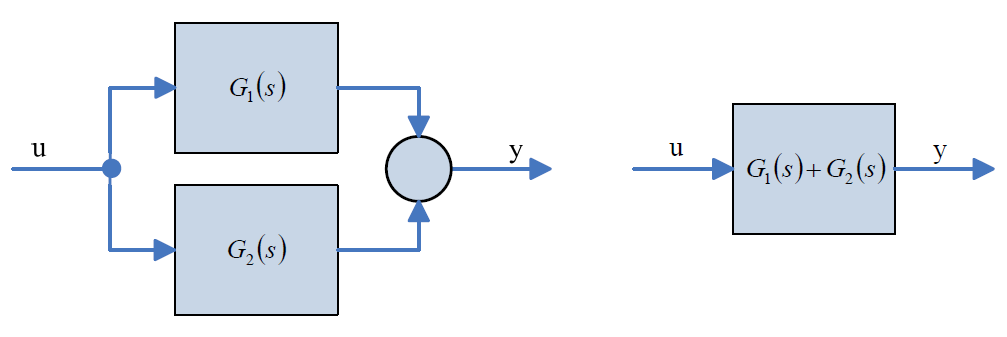
\includegraphics[width = \columnwidth]{imgs/parallelschaltung.png}
\end{figure}
$$
	Y(s) = G_1(s) ⋅ U(s) + G_2(s) ⋅ U(s) = (G_1(s) + G_2(s)) ⋅ U(s)
$$ \\

\textbf{Gegenkopplung:}
\begin{figure}[H]
	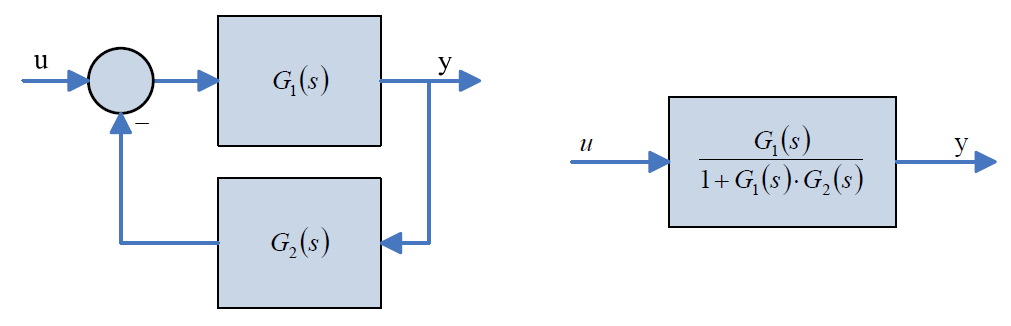
\includegraphics[width = \columnwidth]{imgs/gegenkopplung.png}
\end{figure}
$$
	Y(s) = G_1(s) ⋅ (U(s) - G_2(s) ⋅ Y(s)) \implies Y(s) = \frac{G_1(s)}{1 + G_1(s) ⋅ G_2(s)} ⋅ U(s)
$$ \\

\textbf{Mitkopplung:}
\begin{figure}[H]
	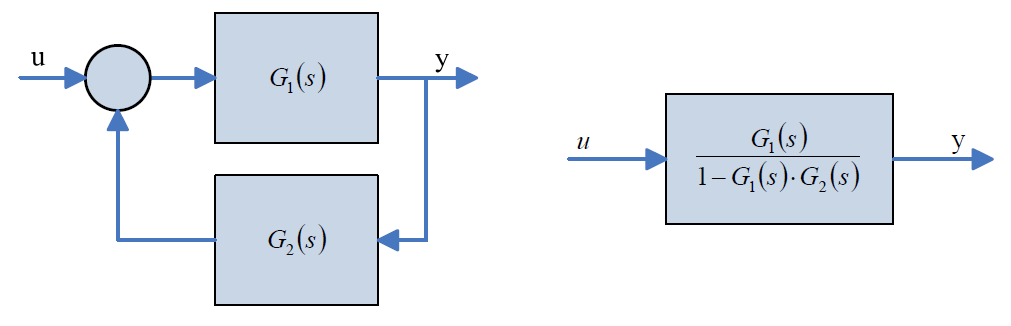
\includegraphics[width = \columnwidth]{imgs/mitkopplung.png}
\end{figure}
$$
	Y(s) = G_1(s) ⋅ (U(s) + G_2(s) ⋅ Y(s)) \implies Y(s) = \frac{G_1(s)}{1 - G_1(s) ⋅ G_2(s)} ⋅ U(s)
$$ \\

\textbf{Vertauschen zweier Blöcke:}
\begin{figure}[H]
	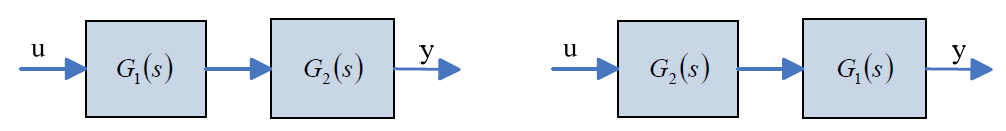
\includegraphics[width = \columnwidth]{imgs/vertauschen_zweier_bloecke.png}
\end{figure}
$$
	Y(s) = G_2(s) ⋅ G_1(s) ⋅ U(s) = G_1(s) ⋅ G_2(s) ⋅ U(s)
$$ \\

\textbf{Vertauschen eines Blockes vor ein Summier-Glied:}
\begin{figure}[H]
	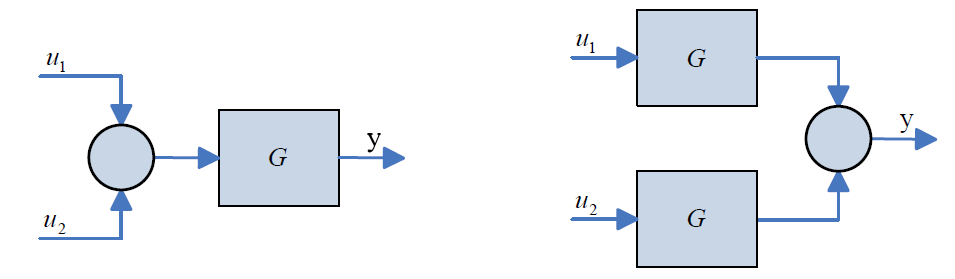
\includegraphics[width = \columnwidth]{imgs/vertauschen_block_vor_summierer.png}
\end{figure}
$$
	Y(s) = G(s) ⋅(U_1(s) + U_2(s)) = G(s) ⋅ U_1(s) + G(s) ⋅ U_2(s)
$$ \\

\textbf{Verlegung eines Blocks hinter ein Summier-Glied:}
\begin{figure}[H]
	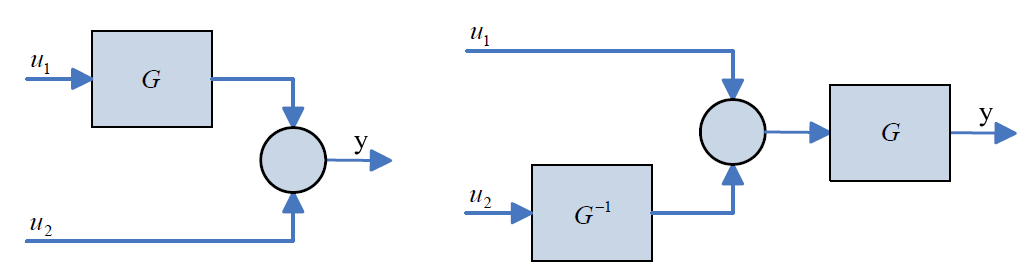
\includegraphics[width = \columnwidth]{imgs/verlegung_block_hinter_summierer.png}
\end{figure}
$$
	Y(s) = G(s) ⋅U_1(s) + U_2(s) = G(s) ⋅ (U_1(s) + \frac{1}{G(s)} ⋅ U_2(s))
$$ \\

\textbf{Verlegung eines Blocks vor eine Verzweigungsstelle:}
\begin{figure}[H]
	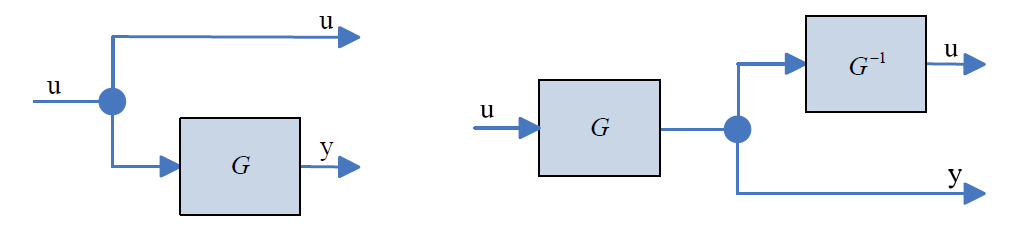
\includegraphics[width = \columnwidth]{imgs/verlegung_block_vor_verzweigung.png}
\end{figure}

\textbf{Verlegung eines Blocks hinter eine Verzweigungsstelle:}
\begin{figure}[H]
	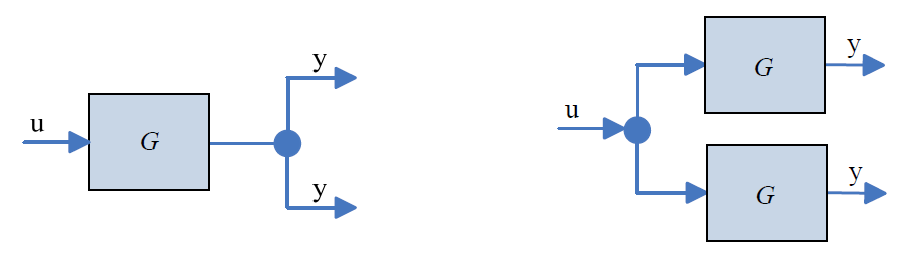
\includegraphics[width = \columnwidth]{imgs/verlegung_block_hinter_verzweigung.png}
\end{figure}

\subsection{Standardregelkreis}
%Sei folgender Regelkreis gegeben:
%\begin{figure}[H]
%	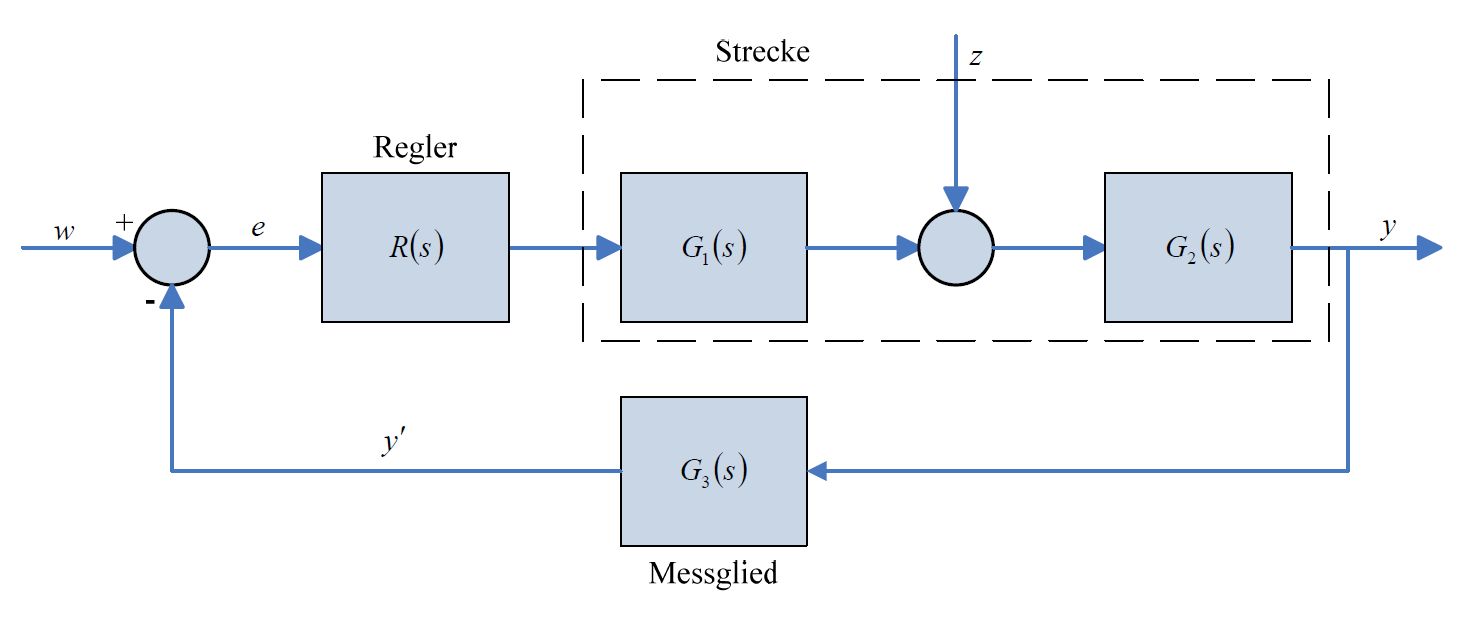
\includegraphics[width = \columnwidth]{imgs/standardregelkreis_1.png}
%\end{figure}
%wobei $G_1(s), G_2(s), G_3(s)$ durch das technische System vorgegeben sind und nur der Regler $R(s)$ frei entworfen werden %kann. \\

Der Standardregelkreis ist definiert als:
\begin{figure}[H]
	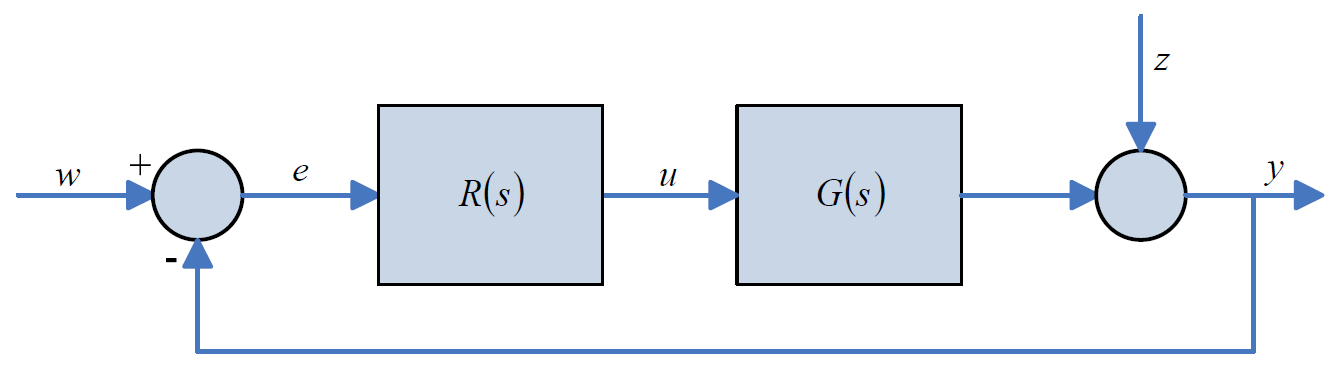
\includegraphics[width = \columnwidth]{imgs/standardregelkreis_2.png}
\end{figure}
mit dem Übertragungsverhalten:
$$
	Y(s) =\underbrace{ \frac{F_o(s)}{1 + F_o(s)}}_{\substack{T(s) \\ \text{Führungsübertra-} \\ \text{gungsfunktion}}} W(s) + \underbrace{\frac{1}{1 + F_o(s)}}_{\substack{S(s) \\ \text{Störübertragungs-} \\ \text{funktion}}} Z(s)
$$
wobei $F_o(s) = G(s)R(s)$ die Übertragungsfunktion des offenen Kreises ist.

\subsubsection{Eigenschaften des Standardregelkreises}
\begin{itemize}
	\item Die Führungsübertragungsfunktion $T(s)$ beschreibt den Einfluss der Führungsgröße $w(t)$ auf die Regelgröße $y(t)$
	\item Die Störübertragungsfunktion bzw. Empfindlichkeitsfunktion $S(s)$ beschreibt den Einfluss der Störgröße $z(t)$ auf $y(t)$
	\item Es gilt: $T(s) + S(s) = 1$
	\item Die Regelabweichung $e$ ist: $E(s) = W(s) - Y(s) = \frac{1}{1 + F_o(s)}W(s) - \frac{1}{1 + F_o(s)} Z(s)$
	\item Die Stellgröße $u$ ist: $U(s) = R(s)E(s) = \frac{R(s)}{1 + F_o(s)}W(s) - \frac{R(s)}{1 + F_o(s)} Z(s)$
\end{itemize}

\subsection{Stabilität des Standardregelkreises}
\subsubsection{Übertragungsstabilität des Standardregelkreises}
Der Standardregelkreis ist genau dann übertragungsstabil bezüglich $S(s)$ und $T(s)$, wenn sämtliche Lösungen der charakteristischen Gleichung 
$$
	F_o(s) + 1 = 0
$$
in der linken komplexen Halbebene liegen.

\subsubsection{Asymptotische Stabilität des Standardregelkreises}
\textbf{Kriterium 1:} \\
Der Standardregelkreis ist genau dann asymptotisch stabil, wenn alle Lösungen der charakteristischen Gleichung 
$$
	Z_0(s) + N_0(s) = 0
$$
in der linken  komplexen Halbebene liegen. Diese Lösungen sind die Systempole der Regelung. \\
Es gilt: 
$$
	Z_0(s) = Z_G(s)Z_R(s), \tab N_0(s) = N_G(s)N_R(s)
$$
$$
	G(s) = \frac{Z_G(s)}{N_G(s)}, \tab R(s) = \frac{Z_R(s)}{N_R(s)}
$$ \\

\textbf{Kriterium 2:} \\
Der Standardregelkreis ist genau dann asymptotisch stabil, wenn alle Lösungen der charakteristischen Gleichung
$$
	F_o(s) + 1 = 0
$$
in der linken komplexen Halbebene liegen und alle eventuelle Pol-Nullstellenkürzungen innerhalb der Strecke ($G(s)$), innerhalb des Reglers ($R(s)$) und zwischen Regler und Strecke ($G(s)R(s)$) ausschließlich links gelegene Pol-Nullstellenpaare betreffen.

\subsubsection{Asymptotische Stabilität beim Reglerentwurf}
Für asymptotische Stabilität der Regelung ist beim Entwurf zu beachten: \\
Rechts oder auf der imaginären Achse gelegene Pole und Nullstellen der Strecke dürfen durch den Regler nicht gekürzt werden.

\subsection{Nyquist-Kriterium}
\subsubsection{Einfaches Nyquist-Kriterium}
Sei $F_o(j \omega)$ die Frequenzgangortskurve des offenen Kreises des Standardregelkreises (auch Nyquist-Kurve genannt) und
seien die unten genannten Voraussetzungen erfüllt. \\
Liegt der Punkt $-1$ links der von der in Richtung wachsender $\omega$ durchlaufenden Frequenzgangortskurve $F_o(j \omega)$, so ist der Regelkreis übertragungsstabil. \\

\textbf{Voraussetzungen:}
\begin{enumerate}
	\item $F_o(s) = \frac{b_0 + b_1s + \dots + b_ms^m}{a_0 + a_1s + \dots + a_ns^n} ⋅ e^{-T_ts}$ mit $m < n$ und $T_t ≥ 0$
	\item Eines der folgenden Voraussetzungen ist erfüllt:
	\begin{enumerate}
		\item Alle Pole von $F_o(s)$ liegen in der linken komplexen Halbebene und $\frac{b_0}{a_0} > 0$
		\item Ein Pol liegt in null, alle anderen Pole von $F_o(s)$ liegen in der linken komplexen Halbebene und $\frac{b_0}{a_1} > 0$
		\item Zwei Pole liegen in null, alle anderen Pole von $F_o(s)$ liegen in der linken komplexen Halbebene und $\frac{b_0}{a_2} > 0$
	\end{enumerate}
\end{enumerate}

\subsubsection{Allgemeines Nyquist-Kriterium}
Sei $F_o(j \omega)$ die Frequenzgangortskurve des offenen Kreises des Standardregelkreises, \\
wobei $F_o(s) = \frac{b_0 + b_1s + \dots + b_ms^m}{a_0 + a_1s + \dots + a_ns^n} ⋅ e^{-T_ts}$ mit $m < n$ und $T_t ≥ 0$ ,\\
sei $r_0$ die Anzahl der in der rechten komplexen Halbebene liegende Pole von $F_o(s)$ und \\
sei $a_0$ die Anzahl der auf der imaginären Achse gelegenen Pole von $F_o(s)$ \\

Der Regelkreis ist genau dann übertragungsstabil, wenn die Winkeländerung $\omega_+$ des Fahrstrahls vom Punkt $-1$ aus betrachtet
$$
	\omega_+ = r_0 \pi + a_0 \frac{\pi}{2}
$$
	beträgt, während die Nyquist-Ortskurve $F_o(j \omega)$ von $\omega = 0$ bis $\omega = ∞$ durchlaufen wird.

\subsubsection{Vereinfachtes Nyquist-Kriterium im Bode-Diagramm}
\begin{figure}[H]
	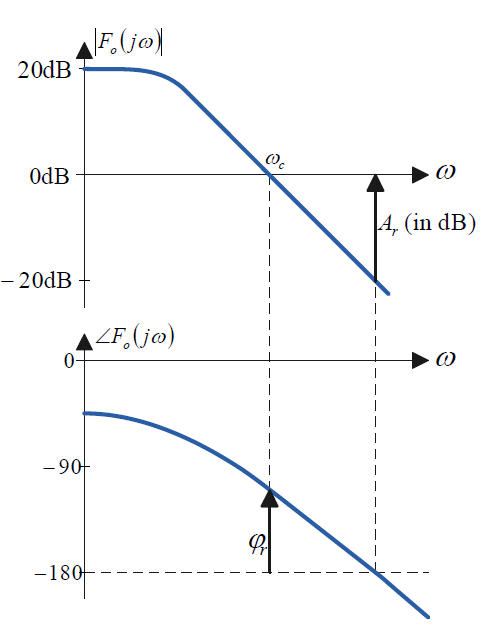
\includegraphics[width = 0.4\columnwidth]{imgs/nyquist_bode.png}
\end{figure}
Sei $F_o(j \omega)$ die Frequenzgangortskurve des offenen Kreises des Standardregelkreises, \\
wobei $F_o(s) = \frac{b_0 + b_1s + \dots + b_ms^m}{a_0 + a_1s + \dots + a_ns^n} ⋅ e^{-T_ts}$ mit $m < n$ und $T_t ≥ 0$ und \\
sei $\omega_c$ die Durchtrittsfrequenz mit $|F_o(j \omega_c)| = 1$. \\
Der Regelkreis ist übertragungsstabil, wenn
$$
	-180° < \angle F_o(j \omega_c) < 0
$$

\paragraph{Phasenreserve} ~\\
Die Phasenreserve $\varphi_r$ ist definiert als:
$$
	\varphi_r = \angle F_o(j \omega_c) + \pi
$$ \\

Ist $\varphi_r > 0$, so ist der Regelkreis übertragungsstabil.

\paragraph{Amplitudenreserve} ~\\
Sei $\omega_a$ die Frequenz, bei der der Phasengang gleich $-180°$ ist, d.h. $\angle F_o(j \omega_a) = -180°$ \\
Die Amplitudenreserver ist definiert als:
$$
	A_r = -|F_o(j \omega_a)|
$$ \\

Ist $A_r > 1$, so ist der Regelkreis stabil

\subsection{Robustheit der Stabilität}
$\varphi_r$ und $A_r$ werden häufig als Maße der Robustheit der Stabilität gegenüber Fehlern oder Veränderungen des Modells $F_o(s)$ verwendet. Faustregel für gute Robustheit:
$$
	\varphi_r > 60° \tab \text{und/oder} \tab A_r > 2
$$ \\

Für gute Robustheit der Stabilität soll der kleinste Abstand
$$
	|d|_{min} = \min_{\omega}|F_o(j \omega) + 1|
$$
der Nyquist-Ortskurve vom Punkt $-1$ möglichst groß sein, Faustregel: 
$$
	|d|_{min} ≥ 0,5
$$

\section{Reglerentwurf}
\subsection{Anforderungen an das Regelverhalten}
\begin{enumerate}
	\item \textbf{Dynamisches Verhalten:}
	\begin{itemize}
		\item Es sind gleichzeitig Schnelligkeit und gute Dämpfung des Einschwingverhaltens (z.B. nach einer Änderung von $w$ oder $z$ anzustreben)
		\item Gleichzeitige Schnelligkeit und gute Dämpfung sind gegenläufig → Kompromiss wird angestrebt
		\item Hohe Dynamik und Robustheit der Stabilität sind gegenläufig
	\end{itemize}
	\item \textbf{Stationäre Genauigkeit:}
	\begin{itemize}
		\item Die Regelabweichung $e(t)$ soll für konstante Störungen als auch für konstante Führungsgrößen für große $t$ gegen null gehen, d.h.
		\begin{itemize}
			\item konstante Störungen sollen stationär ohne Wirkung auf $y$ sein (Störkompensation)
			\item $y$ soll sich stationär auf den konstanten Wert $w$ der Führungsgröße einstellen (Sollwertfolge)
		\end{itemize}
	\end{itemize}
	\item \textbf{Robuste Stabilität:}
	\begin{itemize}
		\item Die zu fordernde Stabilität einer Regelung muss robust gegen Fehler und langsame Veränderungen des Streckenmodells sein. Robustheitsmaße sind u.a.:
		\begin{itemize}
			\item Phasenreserve
			\item Amplitudenreserve
			\item kleinster Abstand der Nyquist-Ortskurve vom Punkt $-1$
			\item Robustheit der Regelgüte
		\end{itemize}
	\end{itemize}
	\item \textbf{Realisierbarkeit des Reglers:}
	\begin{itemize}
		\item Rationale Übertragungsglieder sind realisierbar, wenn für ihre Übertragungsfunktion gilt: Zählergrad $≤$ Nennergrad
	\end{itemize}
	\item \textbf{Einhaltung von Begrenzungen:}
	\begin{itemize}
		\item Systemgrößen dürfen nicht an ihre technisch bedingten Grenzen stoßen.
		\item Häufig betroffen sind die Stellgrößen (z.B: Einhalten eines Maximalwerts)
	\end{itemize}
\end{enumerate}

\subsection{Dynamik, Robustheit der Stabilität und Grenzen der Regelgüte}
Sei $d = F_o(j \omega) + 1$ der Fahrstrahl der Nyquist-Ortskurve $F_o(j \omega)$ (welche dem kritischen Punkt $-1$ am nächsten kommt, wo $d$ den kleinsten Betrag hat). \\
Für die Störübertragungsfunktion $S(s)$ folgt:
$$
	|S(s)| = \begin{cases}
		< 1 & \text{ für } |d| > 1  \tab\text{Störungen werden durch die Regelung gemindert}\\
		= 1 & \text{ für } |d| = 1 \\
		> 1 & \text{ für } |d| < 1  \tab\text{Störungen werden durch die Regelung verstärkt}\\
	\end{cases}
$$

\subsubsection{Bode-Theorem}
Sei der Regelkreis stabil, \\
sei Zählergrad von $F_o(s) + 2 ≤ $ Nennergrad von $F_o(s)$ und \\
sei $p_i$ die in der rechten komplexen Halbebene liegende Pol von $F_o(s)$
Es folgt:
$$
	\begin{array}{ll}
		\int_0^∞ \ln|S(j \omega)| d \omega = 0, & \text{sofern $F_o(s)$ stabil} \\
		\int_0^∞ \ln|S(j \omega)| d \omega = \pi \sum_i  \Re(p_i), & \text{sofern $F_o(s)$ instabil}
	\end{array}
$$

\textbf{Eigenschaften:}
\begin{itemize}
	\item Die Summe der Flächen, wo $|S(s)| < 1|$ gleicht der Summe der Flächen, wo $|S(s) > 1$, sofern $F_o(s)$ stabil ist.
	\item Jede Verbesserung des Störverhaltens in einem gewissen Frequenzbereich muss mit einer Verschlechterung in einem anderen Frequenzbereich bezahlt werden.
	\item Die störungsmindernde Wirkung einer Regelung findet vor allem bei niedrigen Frequenzen statt und endet im Wesentlichen beim kleinsten $\omega$ für das gilt: $|S(j \omega)| = 1$.
\end{itemize}

\textbf{Voraussetzungen für gute Robustheit der Stabilität und gute Dämpfung des Einschwingverhaltens}
\begin{itemize}
	\item Die Ortskurve $F_o(j \omega)$ soll dem Punkt $-1$ nicht sehr nahe kommen bzw. es soll gelten $|S(j \omega)| < 2 = 6dB, \forall \omega$.
	\item Oberhalb von $\omega_1$ soll $F_o(j \omega)$ sehr klein werden, wobei $\omega_1$ das kleinste $\omega$ ist, für das $|S(j \omega)| = 1$ ist.
\end{itemize}

\subsection{Stationäres Verhalten}
\begin{itemize}
	\item Für stationäre Genauigkeit muss zwischen Soll-Ist-wertvergleich und Störeingriff ein Integrierglied enthalten sein. Andernfalls ist die stationäre Regelabweichung $e_{stat} ≠ 0$, kann aber durch Vergrößern von der Verstärkung $V$ kleiner gemacht werden.
	\item Ein Erhöhen der Verstärkung $V$ verschlechtert sich die Robustheit der Stabilität und kann Instabilität bewirken.
	\item Ein Einfügen eines I-Gliedes $\frac{K_I}{s}$ erschwert die Stabilisierung eines Regelkreises und macht ihn langsamer.
\end{itemize}

\subsection{Grundtypen linearer Regler}
Sei im folgenden die Regelabweichung $e(t)$ die Eingangsgröße der Regler und die Stellgröße $u(t)$ die Ausgangsgröße der Regler im Zeitbereich bzw. \\
$R(s)$ die komplexe Übertragungsfunktion des Reglers.

\subsubsection{P-Regler}
\textbf{Definition:}
$$
	\begin{array}{ll}
	\text{Zeitbereich:} & u(t) = K_R e(t) \\
	\text{Bildbereich:} & R(s) = K_R
	\end{array}
$$ \\

\textbf{Wahl der Variablen:} \\
$K_R:$ wird so gewählt, dass Phasen- und Amplitudenreserve groß genug sind, z.B: $A_r > 2, \varphi_r > 60°$ \\

\textbf{Vorteile/Nachteile:}
\begin{itemize}
	\item Vorteile:
	\begin{itemize}
		\item gute Dynamik bei einfachem Regleraufbau
	\end{itemize}
	\item Nachteile:
	\begin{itemize}
		\item stationäre Genauigkeit ist nicht gesichert (außer wenn $G(s)$ ein I-Glied enthält und die Störung erst hinter dem I-Glied eingreift)
	\end{itemize}
\end{itemize}

\subsubsection{I-Regler}
\textbf{Definition:}
$$
	\begin{array}{ll}
	\text{Zeitbereich:} & u(t) = K_I \int_0^t e(\tau) d\tau \\
	\text{Bildbereich:} & R(s) = \frac{K_I}{s}
	\end{array}
$$ \\

\textbf{Wahl der Variablen:} \\
$K_I:$ wird so gewählt, dass Phasen- und Amplitudenreserve groß genug sind, z.B: $A_r > 2, \varphi_r > 60°$ \\

\textbf{Vorteile/Nachteile:}
\begin{itemize}
	\item Vorteile:
	\begin{itemize}
		\item sichert stationäre Genauigkeit
	\end{itemize}
	\item Nachteile:
	\begin{itemize}
		\item tendenziell langsame Dynamik der Regelung
	\end{itemize}
\end{itemize}

\textbf{Bode-Diagramm:}
\begin{figure}[H]
	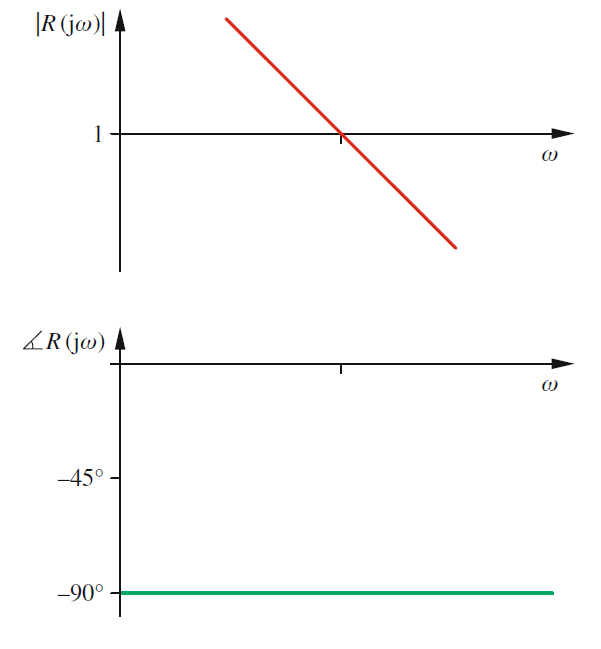
\includegraphics[width = 0.4\columnwidth]{imgs/i-regler.png}
\end{figure}

\subsubsection{PI-Regler}
\textbf{Definition:}
$$
	\begin{array}{ll}
	\text{Zeitbereich:} & u(t) = K_R e(t) + K_I \int_0^t e(\tau) d\tau \\
	\text{Bildbereich:} & R(s) = \frac{K_I}{s} (1 + T_R s) = \frac{K_I}{s} + K_R
	\end{array}
$$ \\

\textbf{Wahl der Variablen:} \\
$K_R = K_I ⋅ T_R$  \\
$T_R =$ größte Nennerzeitkonstante der Strecke \\
$K_I:$ wird so gewählt, dass Phasen- und Amplitudenreserve groß genug sind, z.B: $A_r > 2, \varphi_r > 60°$ \\

\textbf{Vorteile/Nachteile:}
\begin{itemize}
	\item Vorteile:
	\begin{itemize}
		\item schneller als I-Regler
		\item gesicherte stationäre Genauigkeit
	\end{itemize}
%	\item Nachteile:
%	\begin{itemize}
%		\item 
%	\end{itemize}
\end{itemize}

\textbf{Bode-Diagramm:}
\begin{figure}[H]
	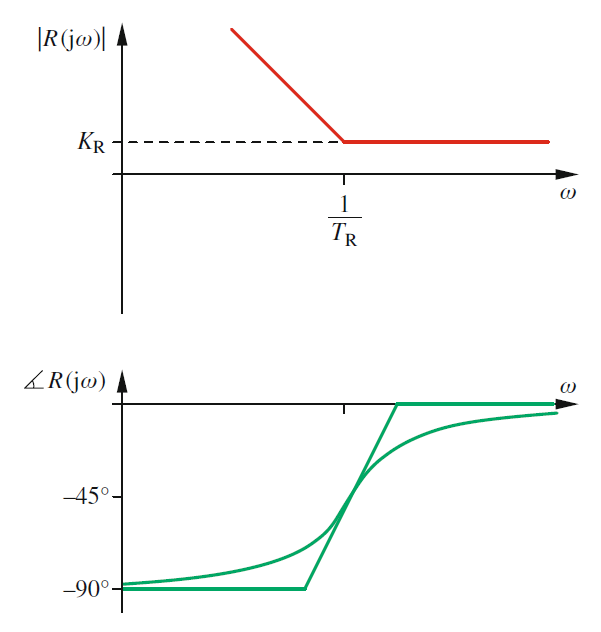
\includegraphics[width = 0.4\columnwidth]{imgs/pi-regler.png}
\end{figure}


\subsubsection{Idealer PD-Regler}
\textbf{Definition:}
$$
	\begin{array}{ll}
	\text{Zeitbereich:} & u(t) = K_R (e(t) + T_R \dot e(t)) = K_R e(t) + K_D \dot e(t) \\
	\text{Bildbereich:} & R(s) = K_R(1 + T_R s) = K_R + K_D s
	\end{array}
$$ \\

\textbf{Wahl der Variablen:} \\
$K_D = K_R + T_R $  \\

\textbf{Vorteile/Nachteile:}
\begin{itemize}
	\item Vorteile:
	\begin{itemize}
		\item hohe Dynamik der Regelung erreichbar
	\end{itemize}
	\item Nachteile:
	\begin{itemize}
		\item Verstärkung der höherfrequenten Störwelligkeit in $e(t)$
		\item D-Anteil kann die Stellgröße in die Begrenzung treiben
	\end{itemize}
\end{itemize}


\subsubsection{Realer PD-Regler}
\textbf{Definition:}
$$
	\begin{array}{ll}
	\text{Bildbereich:} & R(s) = K_R \frac{1 + T_R s}{1 + T_N s}, \tab T_N < T_R
	\end{array}
$$ \\

\textbf{Wahl der Variablen:} \\
$T_R=$ größte Streckenzeitkonstante  \\
$K_R:$ wird so gewählt, dass Phasen- und Amplitudenreserve groß genug sind, z.B: $A_r > 2, \varphi_r > 60°$ \\
$T_N: \frac{T_R}{50} < T_N < \frac{T_R}{5}$ \\

\textbf{Vorteile/Nachteile:}
\begin{itemize}
	\item Vorteile:
	\begin{itemize}
		\item hohe Dynamik erreichbar
	\end{itemize}
	\item Nachteile:
	\begin{itemize}
		\item D-Anteil kann Messstörungen verstärken
		\item D-Anteil kann die Stellgröße in die Begrenzung treiben
	\end{itemize}
\end{itemize}

\textbf{Bode-Diagramm:}
\begin{figure}[H]
	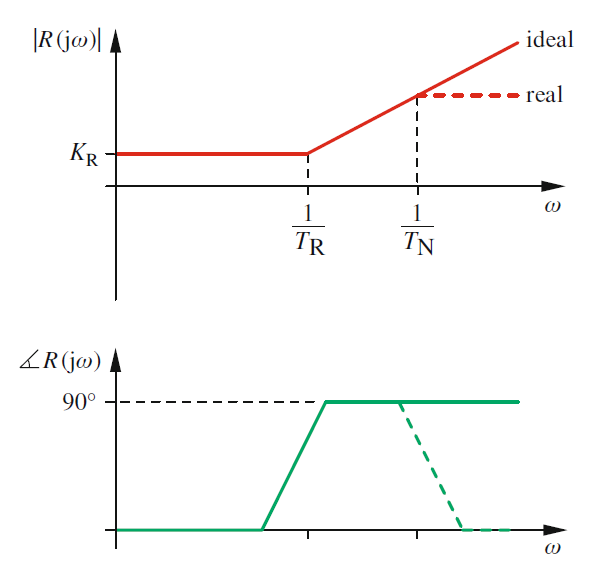
\includegraphics[width = 0.4\columnwidth]{imgs/pd-regler.png}
\end{figure}

\subsubsection{Idealer PID-Regler}
\textbf{Definition:}
$$
	\begin{array}{ll}
	\text{Zeitbereich:} & u(t) = K_R e(t) + K_I \int_0^t e(\tau) d\tau + K_I ⋅ T_{R1} ⋅ T_{R2} ⋅ \dot e(t)\\
	\text{Bildbereich:} & R(s) = K_I(T_{R1} + T_{R2}) + \frac{K_I}{s} + K_I ⋅ T_{R1} ⋅ T_{R2} ⋅ s \\
	& = K_R(1 + \frac{1}{T_I ⋅ s} + T_D s) \\
	& = \frac{K_I}{s}(1 + T_{R1} ⋅ s)(1 + T_{R2} ⋅ s)
	\end{array}
$$ \\


\textbf{Wahl der Variablen:} \\
$K_R = K_I(T_{R1} + T_{R2})$  \\
$T_I = \frac{K_R}{K_I}$ \\
$T_D = \frac{K_I ⋅ T_{R1} ⋅ T_{R2}}{K_R}$ \\

%\textbf{Vorteile/Nachteile}
%\begin{itemize}
%	\item Vorteile:
%	\begin{itemize}
%		\item 
%	\end{itemize}
%	\item Nachteile:
%	\begin{itemize}
%		\item 
%	\end{itemize}
%\end{itemize}

\subsubsection{Realer PID-Regler}
\textbf{Definition:}
$$
	\begin{array}{ll}
	\text{Bildbereich:} & R(s) = \frac{K_I(1 + T_{R1} ⋅ s)(1 + T_{R2} ⋅ s)}{s(1 + T_N ⋅ s)}
	\end{array}
$$ \\

\textbf{Wahl der Variablen:} \\
$T_{R1} =$ größte Streckenzeitkonstante  \\
$T_{R2} =$ zweitgrößte Streckenzeitkonstante \\
$K_I:$ wird so gewählt, dass Phasen- und Amplitudenreserve groß genug sind, z.B: $A_r > 2, \varphi_r > 60°$ \\
$T_N: \frac{T_R}{50} < T_N < \frac{T_R}{5}$ \\

\textbf{Vorteile/Nachteile:}
\begin{itemize}
	\item Vorteile:
	\begin{itemize}
		\item hohe Dynamik
		\item stationäre Genauigkeit
	\end{itemize}
	\item Nachteile:
	\begin{itemize}
		\item D-Anteil kann Messstörungen verstärken
		\item D-Anteil kann die Stellgröße in die Begrenzung treiben 
	\end{itemize}
\end{itemize}

\textbf{Bode-Diagramm:}
\begin{figure}[H]
	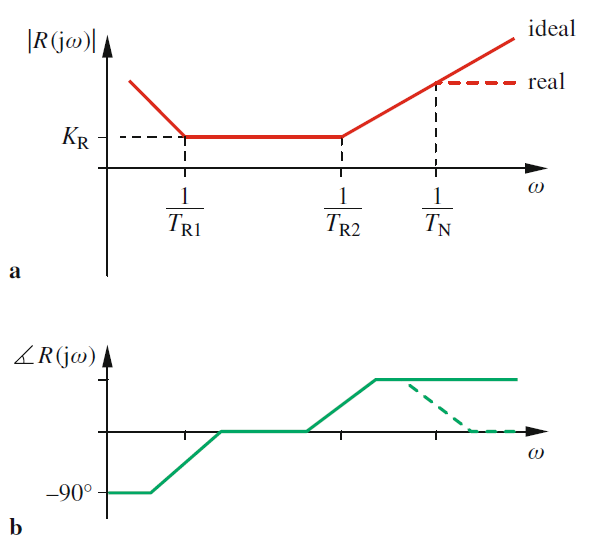
\includegraphics[width = 0.4\columnwidth]{imgs/pid-regler.png}
\end{figure}

\subsubsection{Einstellregeln nach Ziegler und Nichols}
Die Regelstrecke weise rein verzögerndes Verhalten auf (PTn-Glieder mit reellen Polen, Totzeitglieder) und \\
sei $K_{R,krit}$ der Wert für $K_R$ ab dem Dauerschwingungen auftreten, wenn der Regelkreis zunächst nur mit einem P-Regler mit $R(s) = K_R$ betrieben wird und \\
sei $T_{krit}$ die zugehörige Schwingungsdauer. \\

Den gewählten Regler stellt man nach folgender Tabelle ein: \\

\begin{tabular}{l|lll}
	& P-Regler & PI-Regler & PID-Regler \\
	\hline
	$K_R$ & $0,5 ⋅ K_{R,krit}$ & $0,45 ⋅ K_{R,krit}$ & $0,6 ⋅ K_{R,krit}$ \\
	$T_I$ & & $0,85 ⋅ T_{krit}$ & $0,5 ⋅ T_{krit}$ \\
	$T_D$ & & & $0,12 ⋅ T_{krit}$
\end{tabular}

\subsection{Regelungsentwurf im Bodediagramm}
Sei $R_{alt}(s)$ der Regler eines Systems. \\
Weitere Freiheitsgrade zur Gestaltung von Reglern erhält man durch sukzessives Hinzufügen von phasenanhebenden oder phasenabsenkenden Korrekturgliedern $R_{korr}(s)$. \\
Der neue Regler ist dann:
$$
R_{neu}(s) = R_{alt}(s) ⋅ R_{korr}(s)
$$

\subsubsection{Phasenanhebendes Glied (Lead-Glied)}
Die Übertragungsfunktion des phasenanhebenden Glieds ist definiert als:
$$
	R_{korr}(s) = \frac{1 + T_Ds}{1 + T_Vs}, \tab T_D > T_V
$$

\textbf{Eigenschaften:}
\begin{itemize}
	\item Das Korrekturglied kann die Durchtrittsfrequenz und/oder die Phasenreserve der Regelung vergrößern.
	\item Es sind höhere Stellgrößenausschläge zu erwarten
	\item Das Korrekturglied hat die Übertragungsfunktion eines realen PD-Reglers
\end{itemize}

\textbf{Bode-Diagramm:}
\begin{figure}[H]
	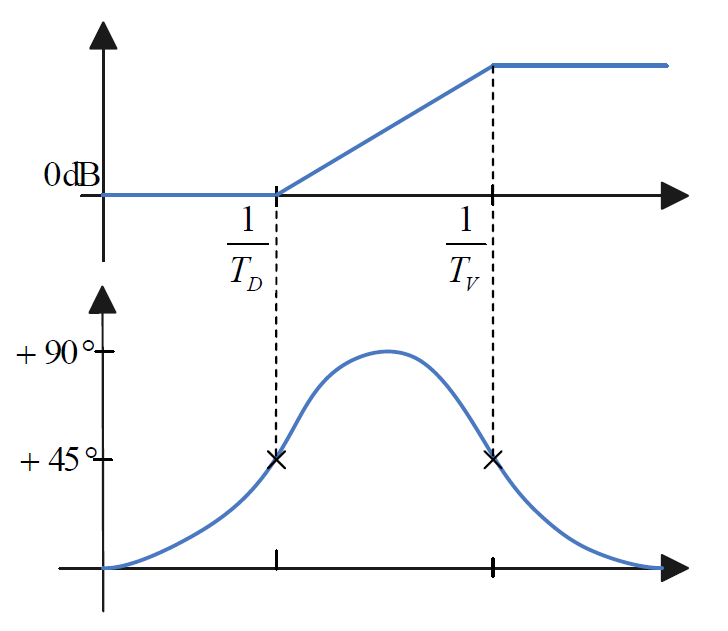
\includegraphics[width = 0.4\columnwidth]{imgs/lead-glied.png}
\end{figure}

\subsubsection{Phasenabsenkendes Glied (Lag-Glied)}
Die Übertragungsfunktion des phasenabsenkenden Glieds ist definiert als:
$$
	R_{korr}(s) = \frac{1 + T_Ds}{1 + T_Vs}, \tab T_D < T_V
$$

\textbf{Eigenschaften:}
\begin{itemize}
	\item Wird typischerweise bei Frequenzen deutlich unterhalb der Durchtrittsfrequenz eingesetzt.
	\item Ermöglicht im offenen Kreis eine Erhöhung der Verstärkung niedriger Frequenzen ohne die Robustheit ungünstig zu verändern
\end{itemize}

\textbf{Bode-Diagramm:}
\begin{figure}[H]
	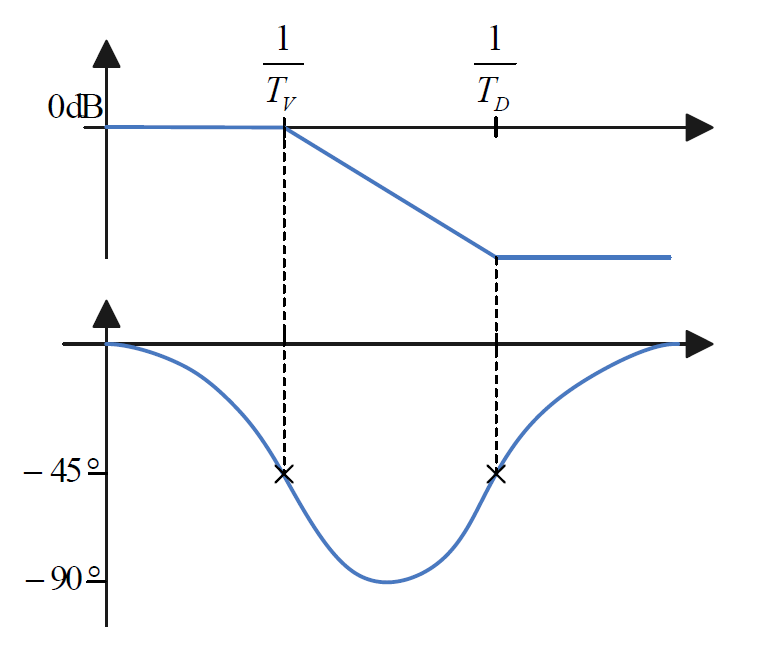
\includegraphics[width = 0.4\columnwidth]{imgs/lag-glied.png}
\end{figure}

\subsection{Kompensationsregler}
Sei ein beliebiges Übertragungsverhalten für den geschlossenen Regelkreis vorgegeben. \\
Durch Kompensation kann der passende Regler ermittelt werden. \\

\textbf{Voraussetzungen:} \\
Sei ein geschlossener Regelkreis gegeben mit zusätzlichen Störeingriff $z_2$ vor der Strecke $G(s)$ und \\
sei $T(s) = \frac{G(s)R(s)}{1 + G(s)R(s)}$ die zugehörige Führungsübertragungsfunktion, \\
sei $S(s) = \frac{1}{1 + G(s)R(s)}$ die zugehörige Störübertragungsfunktion und \\
seien $F_{z_2,y}(s) = \frac{G(s)}{1 + G(s)R(s)}$ und $F_{w,u}(s) = \frac{R(s)}{1 + G(s)R(s)}$ zwei weitere zugehörige Übertragungsfunktionen. \\
Für die Stabilität der Regelung müssen allesamt stabil sein.

\subsubsection{Vorgabe der Führungsübertragungsfunktion T(s)}
\textbf{Realisierbarkeit von R(s):} \\
Der Regler $R(s)$ ist realisierbar, wenn bei der Vorgabe von $T(s)$ gilt:
$$
	\text{Nennergrad}(T) - \text{Zählergrad}(T) ≥ \text{Nennergrad}(G) - \text{Zählergrad}(G)
$$

\textbf{Stationäre Genauigkeit:} \\
Sei stationäre Genauigkeit vorausgesetzt ($T(0) = \frac{Z_T(0)}{N_T(0) = 1}$), dann erhält $R(s)$ einen Pol in null (außer die Strecke besitzt bereits eine Pol in null). \\

\textbf{Stabilität:} \\
Für Stabilität der vier Übertragungsfunktionen ($T(s), S(s), F_{z2,y}(s), F_{w,u}(s)$) müssen alle Pole von $T$ in der linken komplexen Halbebene liegen.
\begin{itemize}
	\item Für die Stabilität von $F_{w,u}(s) = \frac{T(s)}{G(s)}$ müssen eventuell vorhandene rechtes gelegene Nullstellen von $G(s)$ gleichzeitig Zählernullstellen von $T(s)$ sein.
	\item Für die Stabilität von $F_{z2,y}(s) = \frac{T(s)}{R(s)}$ liegt es nahe die Strecke $G(s)$ als stabil vorauszusetzen.
\end{itemize}

\textbf{Definition des Reglers:} \\
Sei $G(s) = \frac{Z_G(s)}{N_G(s)}$ und \\
sei $T(s) = \frac{Z_T(s)}{N_T(s)}$ \\
Der Regler $R(s)$ lässt sich berechnen gemäß:
$$
	R(s) = \frac{T(s)}{G(s)(1 - T(s))} = \frac{Z_TN_G}{Z_G(N_T - Z_T)}
$$

\subsubsection{Vorgabe der Störübertragungsfunktion S(s)}
\textbf{Realisierbarkeit von R(s):} \\
Für die Realisierbarkeit von $R(s)$ ist $S(s)$ anzusetzen als:
$$
	S(s) = \frac{s^q + a_{q-1}s^{q-1} + \dots + a_{q-n+m}s^{q-n+m} + b_{q-n+m-1}s^{q-n+m-1} + \dots + b_1s + b_0}{s^q + a_{q-1}s^{q-1} + \dots + a_1s + a_0}, \tab q ≥ n - m
$$

\textbf{Stationäre Genauigkeit:}
Für stationäre Genauigkeit ist $b_0 = 0$ zu wählen

\textbf{Störübertragungsfunktion minimaler Ordnung} \\
Die Störübertragungsfunktion minimaler Ordnung ($q = n - m$) mit stationärer Genauigkeit ist:
$$
	S(s) = \frac{s^{n-m} + a_{n-m-1}s^{n-m-1} + \dots + a_1s}{s^{n-m} + a_{n-m-1}s^{n-m-1} + \dots + a_1s + a_0}
$$

\textbf{Stabilität:} \\
Für die Stabilität der Regelung müssen $Z_s$ und $N_s$ ($S(s) = \frac{Z_s(s)}{N_s(s)}$) so gewählt werden, dass eventuell vorhandene rechts gelegene Pole und Nullstellen der Strecke sich herauskürzen. \\

\textbf{Definition des Reglers:} \\
Sei $G(s) = \frac{Z_G(s)}{N_G(s)}$ und \\
sei $S(s) = \frac{Z_S(s)}{N_S(s)}$ \\
Der Regler $R(s)$ lässt sich berechnen gemäß:
$$
	R(s) = \frac{1 - S(s)}{G(s)S(s)} = \frac{(N_S - Z_S)N_G}{Z_GZ_S}
$$

\subsubsection{Grenzen der Kompensationsregelung}
Als Indikator für eine zu schnell eingestellte Regelung dient die Übertragungsfunktion von der Störung $z$ auf die Stellgröße $u$:
$$
	F_{zu}(s) = \frac{U(s)}{Z(s)} = - \frac{R(s)}{1 + R(s) G(s)}
$$
Weist sie starke Überhöhungen auf, so ist mit hohen Stellgrößenausschlägen zu rechen.

\subsection{Gütekriterien und optimale lineare Regelung}
\subsubsection{Kennwerte der Sprungantwort}
\begin{itemize}
	\item Überschwingweite: Ziel: möglichst gering
	\item Ausregelzeit: Zeit, die bis zum entgültigen Eintreten der Sprungantwort in einem $\pm 5 \%$-Toleranzbereich um den stationären Endwert verstreicht, Ziel: möglichst kurz.
\end{itemize}
\begin{figure}[H]
	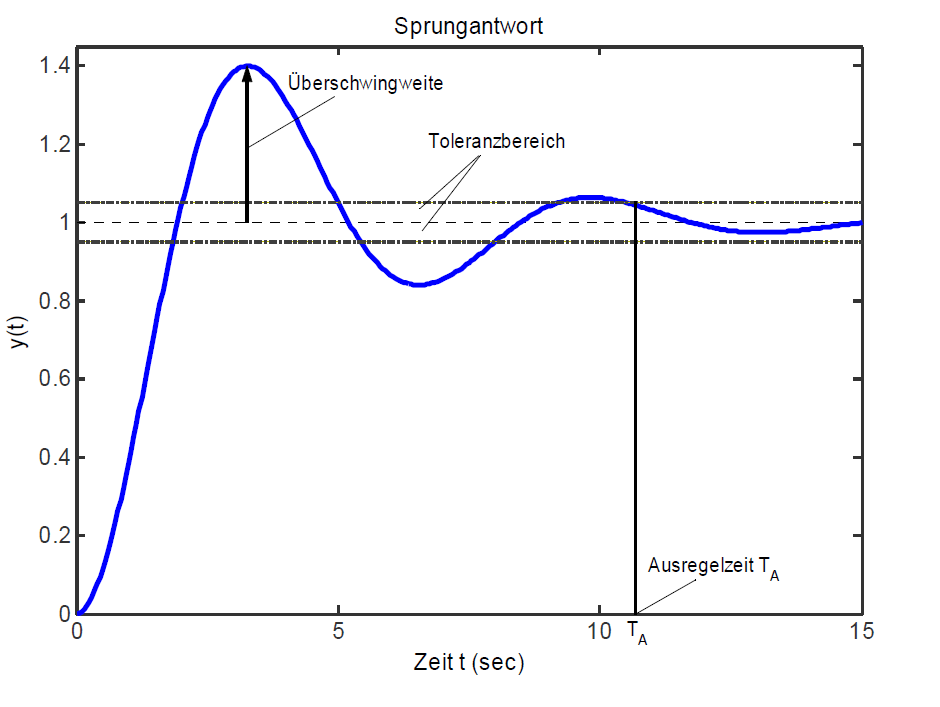
\includegraphics[width = 0.4\columnwidth]{imgs/sprungantwort_kennwerte.png}
\end{figure}

\subsubsection{Integralkriterien im Zeitbereich}
Die Integralkriterien bewerten den gesamten Verlauf der Regelabweichung $e(t)$ bei sprungförmiger Änderung der Führungsgröße.

\paragraph{Betragsregelfläche (IAE, Integral of Absolute Error)} ~\\
$$
	\int_0^∞ |e(t)| dt
$$

Ein kleiner Wert des Integrals bedeutet einen kleinen mittleren Regelfehler.

\paragraph{Zeitgewichtete Betragsregelfläche (ITAE, Integral of Time weighted Absolute Error)} ~\\
$$
	\int_0^∞ t|e(t)| dt
$$

Der Regelfehler wird für kleine Zeiten schwächer gewichtet als für große.

\paragraph{Quadratische Regelfläche (ISE, Integral of Squared Error)} ~\\
$$
	\int_0^∞ e^2(t) dt
$$

Hier gehen große Regelabweichungen besonders stark ein.

\paragraph{Integralkriterium mit Berücksichtigung des Stellgrößenverlaufs}
$$
	\int_0^∞ [e^2(t) + qu^2(t)] dt
$$
wobei $q$ eine positive reelle vorzugebene Konstante ist. \\
Größere Werte für $q$ verringern die Stellgrößenausschläge und verbessern die Robustheit der Stabilität. \\
Kleinere Werte für $q$ erhöhen die Dynamik der Regelung.

\section{Erweiterte Regelstrukturen und Zustandsregelung}
\subsection{Kompensation von Aktor- und Sensorkennlinien}
\begin{itemize}
	\item \textbf{Problem:} Aktoren und Sensoren eines Regelkreises weisen häufig ein-eindeutige nichtlineare Kennlinien auf.
	\item \textbf{Lösung:} Vor- bzw. Nachschalten der inversen Kennlinien
	\begin{itemize}
		\item[→] Lineares Übertragungsverhalten (je ein P-Glied mit Verstärkung eins)
	\end{itemize}
\end{itemize}

\subsection{Zwei-Freiheitsgrade-Regelung}
\textbf{Grundsatz:}
\begin{itemize}
	\item Regelkreise sollen vorrangig auf gutes Störverhalten und Robustheit der Stabilität ausgelegt werden! Das Führungsverhalten kann unabhängig durch eine Steuereinrichtung (Vorsteuerung) manipuliert werden.
\end{itemize}

\begin{figure}[H]
	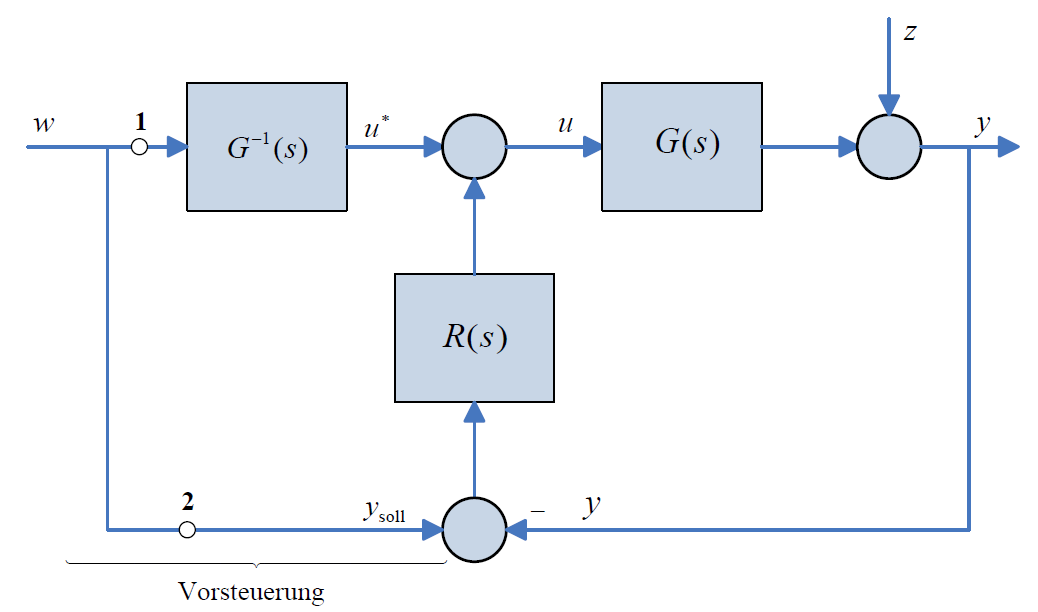
\includegraphics[width=0.5\columnwidth]{imgs/abb7_2.png}
\end{figure}

\textbf{Verhalten der Regelung:}
\begin{itemize}
	\item Keine Störung ($z = 0$) und variable Führungsgröße $w$:
	\begin{itemize}
		\item $e = w - y$ (Regler bleibt inaktiv)
		\item $Y(s) = G(s)G^{-1}(s)W(s) = W(s)$ (ideales Führungsverhalten)
	\end{itemize}
	\item $w = 0$ und $z(t) ≠ 0$:
	\begin{itemize}
		\item Steuereinrichtung bleibt ohne Einfluss.
	\end{itemize}
\end{itemize}

\textbf{Sonderfälle:}
\begin{itemize}
	\item Führungsgröße ist nicht beeinflussbar:
	\begin{itemize}
		\item Einfügen je eines PT$n$-Glieds bei $1$ und $2$ mit \\
		$V(s) = G_{PTn}(s) = \frac{1}{(1 + Ts)^n}$
		\item[→] Führungsverhalten nicht mehr ideal
	\end{itemize}
	\item $G(s)$ besitzt eine rechts gelegene Nullstelle $\eta$:
	\begin{itemize}
		\item Einfügen je eines Glieds bei $1$ und $2$ mit \\
		$V(s) = \frac{1 - \frac 1 q s}{1 + Ts}$
	\end{itemize}
	\item  $G(s)$ enthält eine Totzeit $T_t$:
	\begin{itemize}
		\item Einfügen je eines Glieds bei $1$ und $2$ mit \\
		$V(s) = e^{-T_ts}$
	\end{itemize}
	\item Für alle Fälle gilt:
	\begin{itemize}
		\item Führungsübertragungsverhalten ist: $V(s)$
		\item $Y(s) = V(s) ⋅ W(s) + \frac{1}{1 + G(s) R(s)} Z(s)$
	\end{itemize}
	
\end{itemize}

\subsection{Störgrößenaufschaltung}
\begin{figure}[H]
	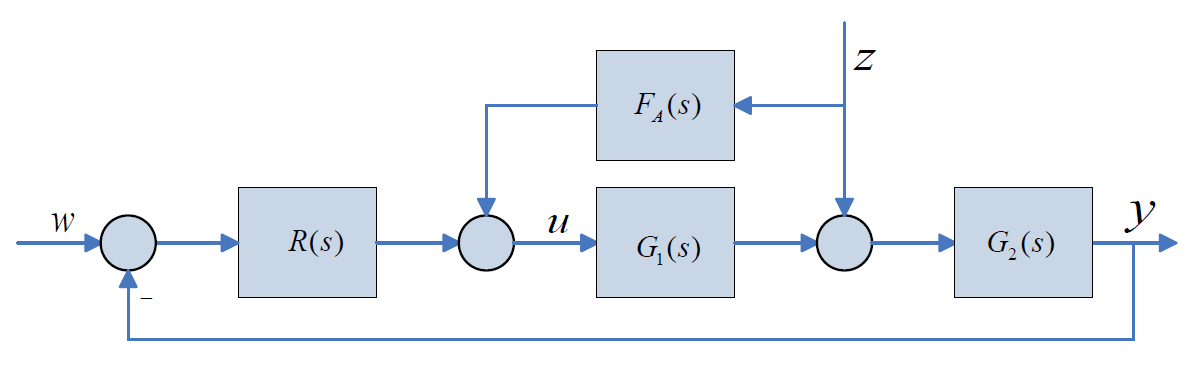
\includegraphics[width=0.7\columnwidth]{imgs/abb7_4.png}
\end{figure}

$$
	Y(s) = \frac{G_2(G_1 F_A + 1)}{1 + G_2 G_1 R} Z(s)
$$

\textbf{Ideale Störgrößenaufschaltung:}
$$
	F_A(s) = -\frac{1}{G_1(s)}, \tab \text{realisierbar, falls Zählergrad $<$ Nennergrad}
$$ ~\\

\textbf{Reale Störgrößenaufschaltung:}
$$
	F_A(s) = -\frac{1}{G_1(s)} ⋅ \frac{1}{(1 + Ts)^n}
$$ ~\\

\textbf{Statische Störgrößenaufschaltung:}
$$
	F_A(s) = -\frac{1}{G_1(0)}
$$

\subsection{Kaskadenregelung}
\begin{figure}[H]
	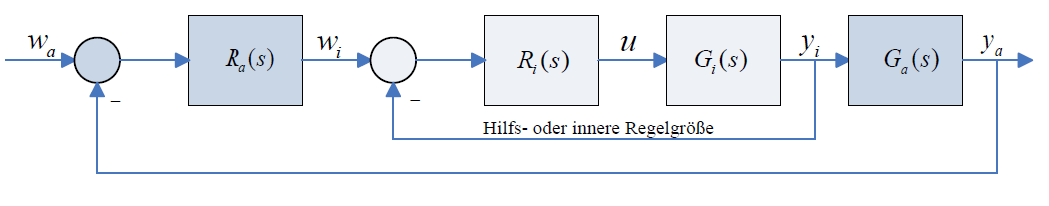
\includegraphics[width=0.8\columnwidth]{imgs/abb7_5.png}
\end{figure}

\textbf{Ziel:}
\begin{itemize}
	\item Schnelleres Reagieren auf Störungen in der inneren Schleife durch Verwenden einer zusätzlichen verfügbaren Messgröße
\end{itemize}

\textbf{Entwurf:}
\begin{enumerate}
	\item Entwurf eines Reglers $R_i(s)$ für die Regelstrecke $G_i(s)$, sodass ein günstiges Störverhalten von $y_i$ bei robuster Stabilität eintritt. \\
	Die Führungsübertragungsfunktion ist:
	$$
		T_i(s) = \frac{Y_i(s)}{W_i(s)} = \frac{G_i R}{1 + G_i R_i}
	$$
	\item Innere Schleife wird mit $G_a(s)$ zu der äußeren Schleife $\bar{G}_a(s) = T_i(s)G_a(s)$
	\item Entwurf eines Reglers $R_a(s)$ für die Regelstrecke $\bar G_a(s)$, sodass ein günstiges Störverhalten von $y_a$ mit zumeist stationärer Genauigkeit eintritt. \\
\end{enumerate}

\subsection{Kaskade aus Zwei-Freiheitsgrade-Regelung}
\begin{figure}[H]
	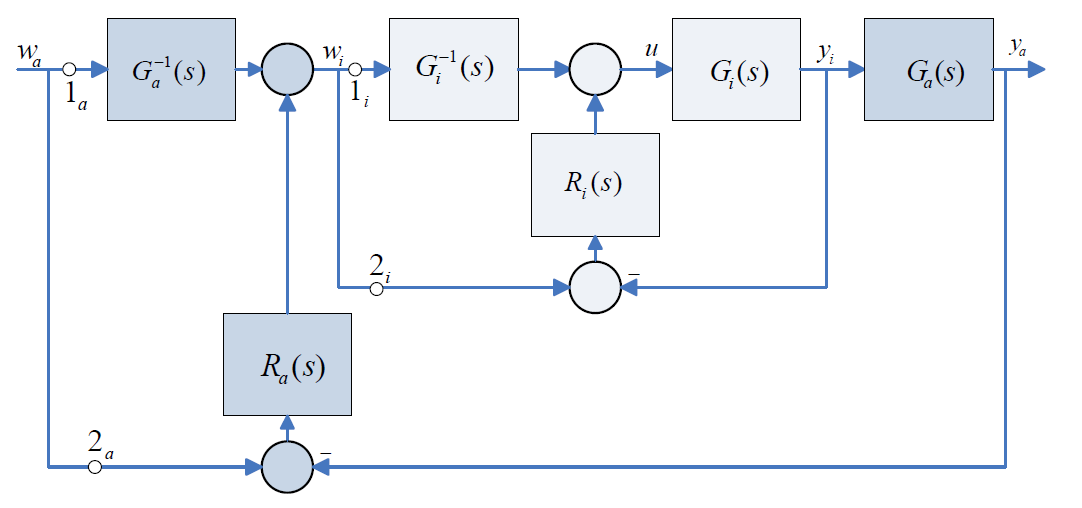
\includegraphics[width=0.8\columnwidth]{imgs/abb7_8.png}
\end{figure}

\textbf{Ziel:}
\begin{itemize}
	\item Kombination der Vorteile der Kaskadenregelung und der Zwei-Freiheitsgrade-Regelung
\end{itemize}

\textbf{Eigenschaften:} ~\\
\begin{tabularx}{\columnwidth}{llX}
	Bezeichnung & Var. & Beschreibung \\
	\hline
	Regler (innere Schleife) & $R_i$ & Wird für gutes Störverhalten der Strecke $G_i$ ausgelegt. \\
	Vorsteuerung (innere Schleife) & $G_i^{-1}$ & Sorgt für ideales Führungsverhalten $T_i(s) = 1$ der inneren Schleife \\
	Regler (äußere Schleife) & $R_a$ & wird für gutes Störverhalten der Strecke $G_a$ ausgelegt \\
	Vorsteuerung (äußere Schleife) & $G_a^{-1}$ & sorgt für ideales Führungsverhalten der äußeren Schleife \\
\end{tabularx}

\subsection{Zustandsregelung}
\subsubsection{Konstante Zustandsrückführung und Vorsteuerung}
\label{zustandsrueckfuehrung}
\begin{figure}[H]
	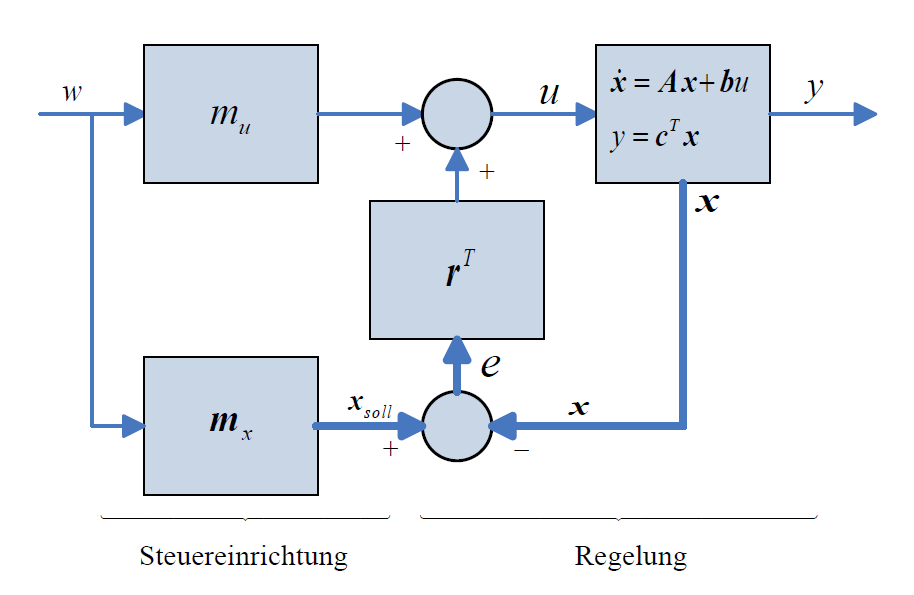
\includegraphics[width=0.7\columnwidth]{imgs/abb7_10.png}
\end{figure}

Sei die Strecke in Zustandsdarstellung. \\

\textbf{Formeln}
$$
	\dot x(t) = Ax(t) + bu(t)
$$
$$
	y(t) = c^Tx(t)
$$
$$
	u(t) = r^Te(t) + m_uw(t) = r^T(m_xw(t)-x(t)) + m_u w(t)
$$
$$
	G_{wy}(s) = \frac{Y(s)}{W(s)} = c^T(sI-A_r)^{-1}b_r \tab (\text{Komplexe Übertragungsfunktion:})
$$ ~\\

\textbf{Variablen} ~\\
\begin{tabularx}{\columnwidth}{ll}
	Bezeichnung & Var. \\
	\hline
	P-Glied Verstärkung & $m_u \in \mathbb{R}$ \\
	\tab - & $m_x \in \mathbb{R}^{n \times 1}$  \\
	Zustands-Sollverlauf & $x_{soll}(t) = m_xw(t) \in \mathbb{R}^{n \times 1}$  \\
	vektorielle Regelabweichung & $e(t) = \vect{e_1(t) \\ \vdots \\ e_n(t)} = x_{soll}(t) - x(t)$  \\
	Faktoren & $r^T = \vect{r_1 & \dots & r_n}$ \\
	Systemordnung & $n$ (Zahl der Elemente von $x$)
\end{tabularx} ~\\

\textbf{Anforderungen} ~\\
\textbf{1. Anforderung:} ~\\
Im stationären Fall (d.h. im eingeschwungenen Zustand mit $\dot x = 0$) soll die Regelgröße $y$ den Sollwert $w$ annehmen, also $y = w$, und die vektorielle Regelabweichung $e = x_{soll} − x$ soll null werden, also $x = x_{soll}$ \\
Es folgt:
$$
	\vect{A & b \\ c^T & 0} ⋅ \vect{m_x \\ m_u} = \vect{0 \\ 1}
$$

\textbf{2. Anforderung:} ~\\
Das dynamische Verhalten der Regelung soll asymptotisch stabil sein und eine gewünschte Schnelligkeit und Dämpfung aufweisen. \\
Es folgt:
$$
	\dot x(t) = (A - br^T)x(t)
$$
Für asymptotische Stabilität müssen die Eigenwerte $p_1, \dots, p_n$ der Matrix $A - br^T$ (Regelungseigenwerte) in der linken komplexen Halbebene liegen. \\

Entwurf:
\begin{enumerate}
	\item $\det(sI - A + br^T) = s^n + c_{n-1}(r_1, \dots, r_n) ⋅ s^{n-1} + \dots + c_0(r_1, \dots, r_n)$, \tab wobei $c_i = f(r_1, \dots, r_n)$
	\item $P(s) = (s - p_1) ⋅ \dots ⋅ (s - p_n) = s^n + a_{n-1}s^{n - 1} + \dots + a_1s + a_0$, \tab wobei $p_i$ die gewünschten Eigenwerte sind
	\item Auflösen nach $r_1, \dots, r_n$: \\
	$$\begin{array}{c}
		c_{n-1}(r_1, \dots, r_n) = a_{n-1} \\
		\vdots \\
		c_0(r_1, \dots, r_n) = a_0
	\end{array}$$
\end{enumerate}

\textbf{Eigenschaften}
\begin{itemize}
	\item Alle Eigenwerte und somit die vollstädige Dynamik der Regelung können vom Entwerfer vorgegeben werden. Dazu ist die Messung aller n Zustandsvariablen nötig (oder deren Schätzung durch einen sogenannten Zustandsbeobachter).
	\item Die Entwürfe des Reglers $r^T$ und der Vorsteuerung $m_u, m_x$ geschehen unabhängig.
	\item Die Vorgabe der Eigenwerte erlaubt eine sehr gezielte und umfassende Gestaltung der gesamten Systemdynamik. Je weiter links die Regelungseigenwerte platziert werden, desto schneller das Regelverhalten, desto höher	aber auch die Stellgrößenausschläge.
\end{itemize}

\paragraph{Berücksichtigung des Eingriffs einer äußeren Störung $z(t)$}
$$
	\dot x = (A - br^T) x + b (r^T m_x + m_u) w + \bar e z
$$
$$
	Y(s) = c^T(sI-A_r)^{-1}b_rW(s) + c^T(sI-A_r)^{-1}\bar eZ(s)
$$

\subsubsection{Zustandsbeobachter}
\begin{figure}[H]
	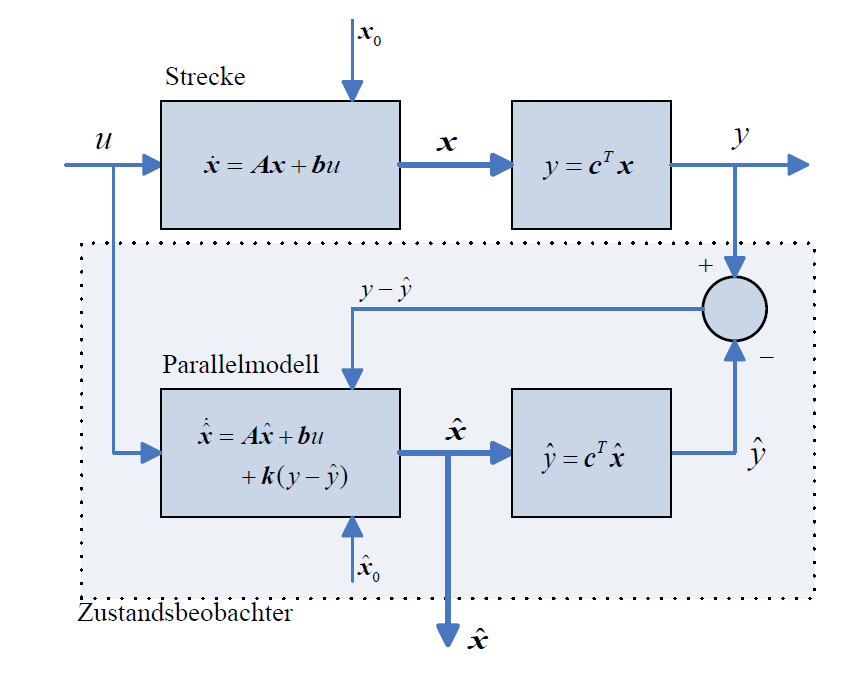
\includegraphics[width=0.7\columnwidth]{imgs/abb7_12.png}
\end{figure}

\textbf{Ziel:}
\begin{itemize}
	\item Schätzung des Zustandsvektors $x$ (, da $x(t)$ nicht messbar)
	\item Einführung eines Vektors $\hat x$ als Schätzung für $x$
\end{itemize} ~\\

\textbf{Formeln:} ~\\
$
	\begin{array}{ll}
		\text{Zustandsschätzung} & \dot {\hat x} = A \hat x + bu + k(y - \hat y) = (A + kc^T)\hat x + bu + ky\\
		\text{Schätzung für }y & \hat y = c^T\hat x \\
		\text{Schätzfehler} & \tilde{x} = x - \hat x \\
		\text{Ableitung des Schätzfehlers} & \dot{\tilde x} = (A - kc^T)\tilde x = A_k \tilde x
	\end{array}
$ \\~\\

\textbf{Entwurf:}
\begin{enumerate}
	\item $\det(sI - A + kc^T) = s^n + c_{n-1}(k_1, \dots, k_n) ⋅ s^{n-1} + \dots + c_0(k_1, \dots, k_n)$, \tab wobei $c_i = f(k_1, \dots, k_n)$
	\item $P(s) = (s - p_1) ⋅ \dots ⋅ (s - p_n) = s^n + a_{n-1}s^{n - 1} + \dots + a_1s + a_0$, \tab wobei $p_i$ die gewünschten Eigenwerte sind
	\item Auflösen nach $k_1, \dots, k_n$: \\
	$$\begin{array}{c}
	c_{n-1}(k_1, \dots, k_n) = a_{n-1} \\
	\vdots \\
	c_0(k_1, \dots, k_n) = a_0
	\end{array}$$
\end{enumerate} ~\\

\textbf{Eigenschaften:}
\begin{itemize}
	\item $\lim_{t → ∞} \hat x = x$
	\item Der Zustandsbeobachter wird vollständig im Digitalrechner	realisiert.
	\item Der Zustandsbeobachter kann auf Fälle erweitert werden, in denen nicht nur eine, sondern mehrere Messgrößen zur Verfügung stehen.
	\item Je weiter links die Eigenwerte liegen, desto schneller klingt der Schätzfehler ab, desto empfindlicher wird die Schätzung aber gegenüber Störungen durch Messrauschen.
\end{itemize}

\subsubsection{Zustandsrückführung mit Beobachter}
\begin{figure}[H]
	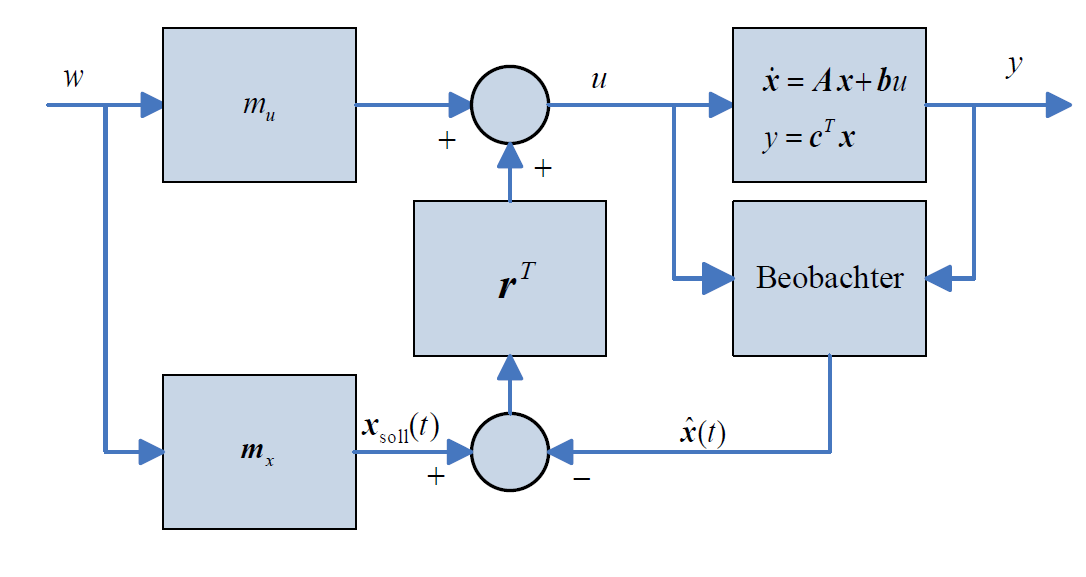
\includegraphics[width=0.7\columnwidth]{imgs/abb7_13.png}
\end{figure}

\textbf{Ziel:}
\begin{itemize}
	\item Verwendung der Zustandsrückführung trotz nicht-messbarer Zustandsvariablen
\end{itemize}

\subsubsection{Mehrgrößenregelung im Zustandsraum}
\begin{figure}[H]
	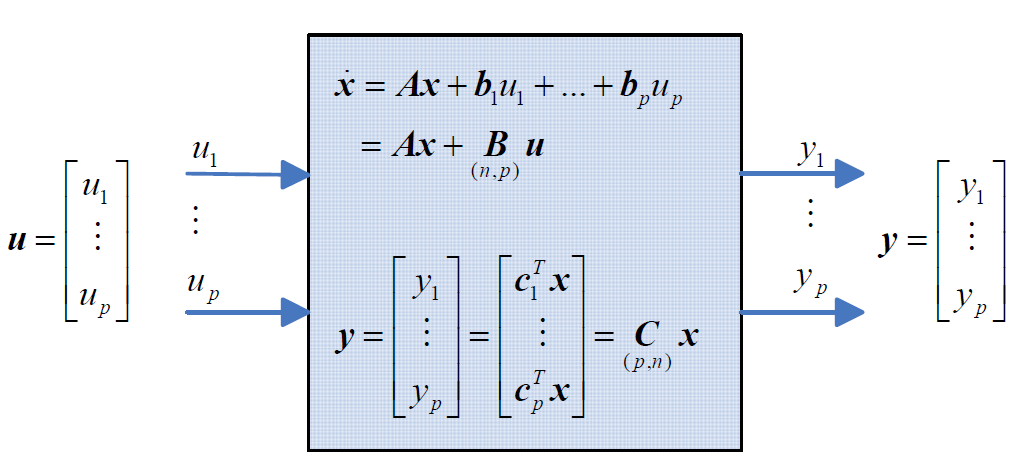
\includegraphics[width=0.7\columnwidth]{imgs/abb7_14.png}
\end{figure}
\begin{figure}[H]
	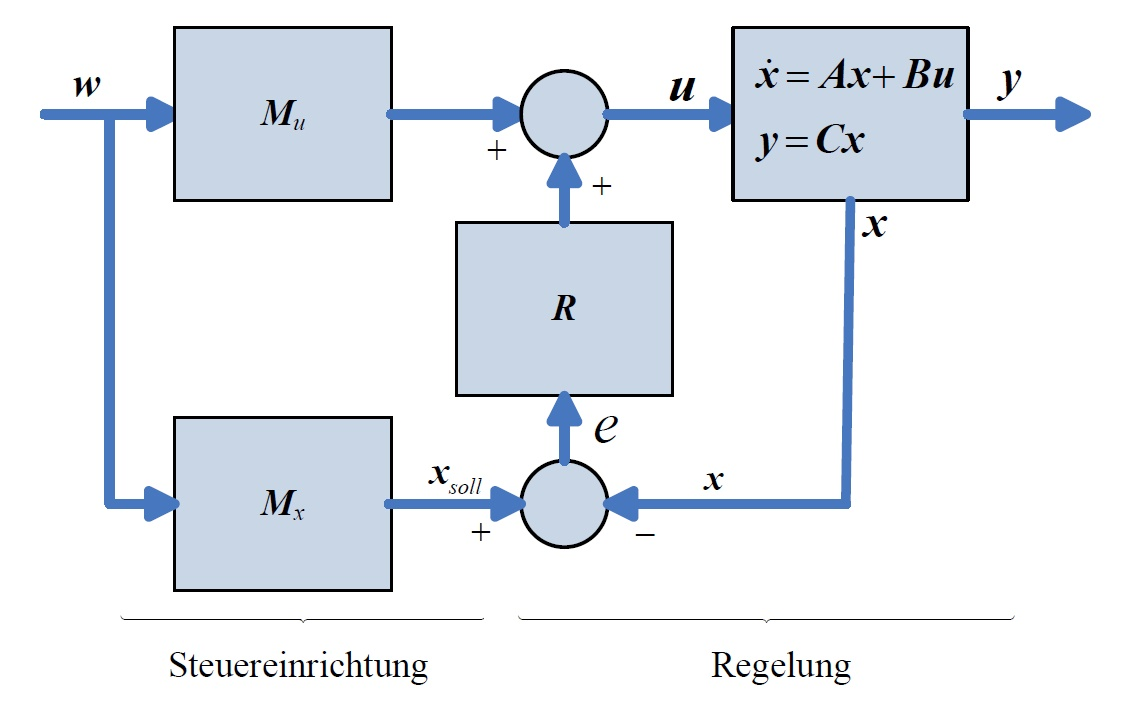
\includegraphics[width=0.7\columnwidth]{imgs/abb7_15.png}
\end{figure}

\textbf{Ziel:}
\begin{itemize}
	\item Verwenden von mehreren Stell- und Regelgrößen
\end{itemize} ~\\

\textbf{Formeln:}
$$
	\dot x = Ax + Bu
$$
$$
	y = Cx
$$ 
$$
	Y(s) = C(sI-A_R)^{-1} B_R W(s) + C(sI-A_R)^{-1} E Z(s) \tab A_R = A - BR, B_R = B(RM_x + M_u)
$$~\\

\textbf{Variablen} ~\\
\begin{tabularx}{\columnwidth}{llllll}
	Stellgrößen & $u = \vect{u_1 \\ \vdots \\ u_p} \in \mathbb{R}^{p \times 1}$ \\
	Regelgrößen & $y = \vect{y_1 \\ \vdots \\ y_n} \in \mathbb{R}^{p \times 1}$ \\
	 $B \in \mathbb{R}^{n \times p}$, 
	 & $C \in \mathbb{R}^{p \times n}$, 
	 & $R \in \mathbb{R}^{p \times n}$, 
	 & $M_u \in \mathbb{R}^{p \times p}$, 
	 & $M_x \in \mathbb{R}^{n \times p}$
\end{tabularx} ~\\

\textbf{Entwurf:}
\begin{enumerate}
	\item $
	\vect{A & B \\ C & 0} \vect{M_x \\ M_u} = \vect{0 \\ I}
	$
	\item Bestimmung der Reglermatrix $R$ wie in \ref{zustandsrueckfuehrung}
\end{enumerate}

\subsection{Nichtlineare Zustandsregelung durch Ein-/Ausgangslinearisierung}
\textbf{Ziel:}
\begin{itemize}
	\item Verfahren, mit dem man gewisse nichtlineare Strecken durch ein nichtlineares Zustandsrückführungsgesetz derart regeln kann, dass lineares Ein-/Ausgangsverhalten (lineares Führungsverhalten) eintritt.
\end{itemize}

\textbf{Vorgehen:}
\begin{enumerate}
	\item Formulieren der nichtlinearen Streckenbeschreibung in der Zustandsdarstellung: \\
	$\dot x = a(x) + b(x) u$ \\
	$y = c(x) := c_0(x)$
	\item Ableiten von $y$ nach $x$ solange bis $u$ auftaucht: \\
	Wiederhole solange bis $b_q(x) ≠ 0$, starte mit $q = 0$, inkrementiere $q$ nach jedem Schritt um 1\\
	$y^{(q)} = \frac{\partial c_{q-1}}{\partial x_1} \dot x_1 + \dots + \frac{\partial c_{q-1}}{\partial x_n} \dot x_n = c_q(x) + b_q(x) u$
	\item Einsetzen in Wunschdifferentialgleichung (hier: $y^{(q)} + a_{q - 1}y^{(q-1)} + \dots + a_1 \dot y + a_0y = a_0 w$): \\
	$c_q(x) + b_q(x) u + a_{q-1} y^{(q-1)} + \dots + a_1 \dot y + a_0 y = a_0 w$
	\item Auflösen nach $u$: \\
	$u = \frac 1 {b_q(x)} (-c_q(x) - a_{q-1} y^{(q-1)} - a_1 \dot y - a_0 y + a_0 w)$
	\item Einsetzen von $y^{(i)} = c_i(x)$ aus Schritt 2: \\
	$u = \frac 1 {b_q(x)} (-c_q(x) - a_{q-1} c_{q-1}(x) - a_1 c_1(x) - a_0 c(x) + a_0 w)$
\end{enumerate}
Es folgt:
$$
	Y(s) = \frac{a_0}{s^q + a_{q-1}s^{q-1} + \dots + a_0} W(s)
$$

\textbf{Eigenschaften:}
\begin{itemize}
	\item Der sogenannte relative Grad $q$ ist bei technisch sinnvollen Systemen stets kleiner oder gleich der Systemordnung $n$.
	\item Der Entwurf sichert lineares Ein-/Ausgangsverhalten.
	\item Die Dynamik der Zustandsvariablen bleibt nichtlinear.	Falls $q < n$ ist, können nur $q$ Pole vorgegeben werden. Die verbleibenden $n − q$ Freiheitsgrade der Systemdynamik bleiben im Systeminnern „versteckt“. Diese versteckte, man sagt auch interne Dynamik, kann instabiles Verhalten von Zustandsvariablen aufweisen. Falls $q = n$ ist und alle oben verwendeten Ausdrücke frei von Singularitäten sind (zumindest im interessierenden Bereich des Zustandsraums), dann darf man im Allgemeinem von einem stabilen Systemverhalten ausgehen.
\end{itemize}

\section{Digitale Realisierung}
\begin{figure}[H]
	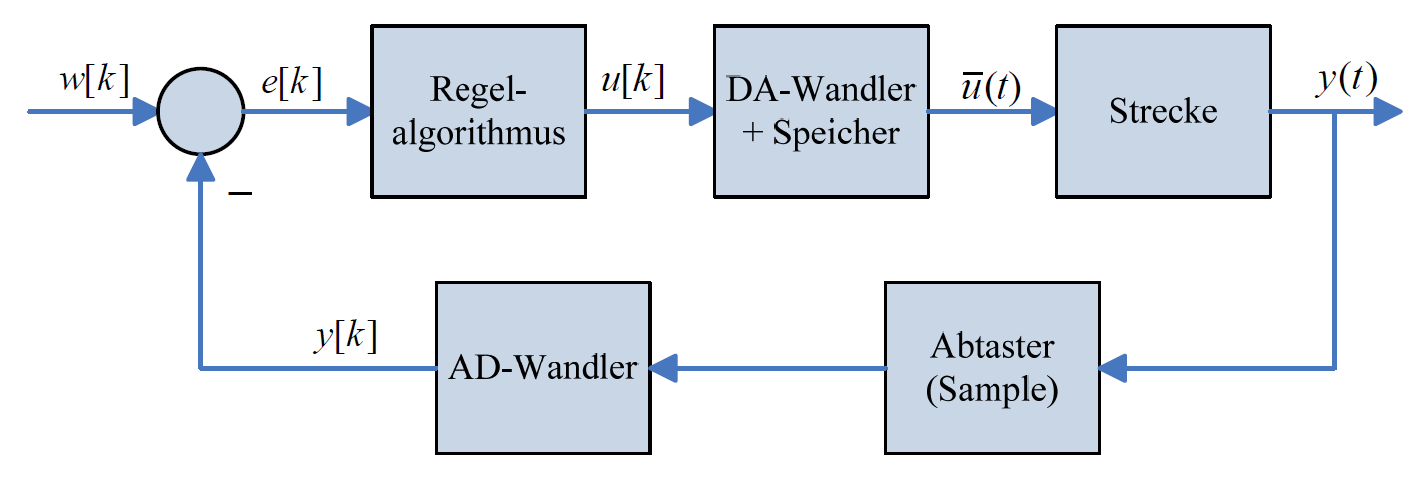
\includegraphics[width=\columnwidth]{imgs/abb8_1.png}
\end{figure}

\begin{itemize}
	\item \textbf{Abtaster:} Entnimmt dem elektrischen Messsignal $y$ zu den diskreten Zeiten $t = 0, T, 2T, \dots$ dessen Wert (Samples).
	\item \textbf{Analog-Digital-Wandler (AD-Wandler):} Wertediskretisiert die Samples (Wandelt die zeitdiskreten Messwerte in Binärzahlen um).
	\item \textbf{Digital-Analog-Wandler (DA-Wandler):} Wandelt den jeweils aktuellen Wert $u[k]$ in einen elektrischen Spannungswert, welcher bis zum nächsten Abtastzeitpunkt gehalten wird. \\
	→ treppenförmiges Stellgrößensignal $\bar u(t)$
	\item \textbf{Abtastzeit $T$:} Zeit zwischen zwei Samples.
\end{itemize}



\subsection{Tustin-Transformation}
Sei $z ⋅ u[k] = u[k + 1]$ sowie $z^{-1} ⋅ u[k] = u[k-1]$ \\
Die Tustin-Transformation ist definiert als:
\renewcommand{\arraystretch}{2}
$$
	\begin{array}{lll}
		R(z) = \frac{u[k]}{e[k]} = \frac{T(1+z^{-1})}{2(1 + z^{-1})} & \text{entspricht} & R(s) = \frac 1 s \\
		R(z) = \frac{u[k]}{e[k]} = \frac{2(1-z^{-1})}{T(1 + z^{-1})} & \text{entspricht} & R(s) = s \\	
	\end{array}
$$
\renewcommand{\arraystretch}{1.5}
\subsection{Glieder und Regler}
Sei $T$ die Abtastzeit zwischen zwei Samples und \\
sei $e[k]$ die Regelabweichung zum Zeitpunkt $t = kT$ \\

\subsubsection{Digitales I-Glied}
Sei das I-Glied definiert als $R(s) = \frac 1 s$ \\
Der Algorithmus für das I-Glied ist definiert als:
$$
u[k] = u[k-1] + \frac T 2 (e[K-1] + e[k])
$$

\subsubsection{Diskreter PD-Regler}
Sei der PD-Regler definiert als $R(s) = K_R(1 + T_R s)$ \\
Der Algorithmus für den PD-Regler ist definiert als:
$$
	u[k] = -u[k-1] + d_0e[k] + d_1e[k-1]
$$
wobei \tab $d_0 = \frac{K_R}{T}(T + 2T_R)$, \tab $d_1 = \frac{K_R}{T}(T - 2T_R)$

\subsubsection{Diskreter PID-Regler}
Sei der PID-Regler definiert als $R(s) = K_R(1 + \frac{1}{T_I s} + T_D s)$ \\
Der Algorithmus für den PID-Regler ist definiert als:
$$
	u[k] = u[k-1] + d_0e[k] + d_1e[k-1] + d_2e[k-2]
$$
wobei \tab $d_0 = K_R(\frac{T_D}{T} + \frac{T}{T_I} + 1)$, \tab $d_1 = -K_R(1 + 2\frac{T_D}{T})$, \tab $d_2 = K_R \frac{T_D}{T}$


\subsection{Zeitdiskrete Zustandsdarstellung}
Sei ein System in Zustandsdarstellung gegeben mit $\dot x = Ax + bu$ und $y = c^T x$ \\
Die zeitdiskrete Zustandsdarstellung ist definiert als:
$$
	x[k+1] = \Phi x[k] = \beta u[k]
$$
$$
	y[k] = c^T x[k]
$$
wobei
$$
	\Phi = e^{AT}
$$
$$
	\beta = A^{-1}(\Phi - I) b
$$












\appendix

\pagebreak
\section{Mathematische Grundlagen}
\subsection{Komplexe Zahlen}
\subsubsection{Definition}
Eine komplexe Zahl $z \in \mathbb{C}$ ist definiert als:
$$
	z = x + jy
$$
wobei $x, y \in \mathbb{R}$ und
$j = \sqrt{-1}$ ist die imaginäre Einheit. \\

Der Real- und Imaginärteil ist definiert als:
$$
	\Re(z) = x, \tab 	\Im(z) = y
$$

\subsubsection{Konjugiert komplexe Zahl}
Sei $z \in \mathbb{C}$. \\
Die zu $z$ konjugiert komplexe Zahl $z^*$ ist:
$$
	z^* = x - jy
$$

\subsubsection{Betrag einer komplexen Zahl}
Sei $z \in \mathbb{C}$. \\
Der Betrag von $z$ ist:
$$
	|z| = \sqrt{x^2 + y^2}
$$

\subsubsection{Euler-Formel}
$$
e^{j\varphi} = \cos \varphi + j \sin \varphi
$$

\subsubsection{Polarkoordinaten}
Sei $z \in \mathbb{C}$. \\
$z$ angegeben in Polarkoordinaten ist definiert als:
$$
	z = |z|(\cos \varphi + j \sin \varphi) = |z|e^{j\varphi}
$$
wobei \\
$\varphi = \arg(z) = \begin{cases}
	\arctan(\frac y x) & $für $x > 0 \\
	\pi + \arctan(\frac y x) & $für $x < 0
\end{cases}
$

\subsubsection{Addition, Multiplikation}
Sei $z_1, z_2 \in \mathbb{C}$. \\
Es folgt:
$$
	z_1 + z_2 = (x_1 + x_2) + j(y_1 + y_2)
$$
$$
	z_1 ⋅ z_2 = (x_1x_2 - y_1y_2) + j(x_1y_2 + y_1x_2)
$$
$$
	z_1 ⋅ z_2 = |z_1| ⋅ |z_2| ⋅ e^{j(\varphi_1 + \varphi_2)}
$$

\subsection{Partialbruchzerlegung}
Sei $R(s) = \frac{b_ns^n + \dots + b_1s + b_0}{a_ms^m + \dots + a_1s + a_0}$ \\

1. Finde alle Polstellen $p_i$ von $R(s)$ \\

2. Setze Partialbrüche an: \\
$R(s) = G_1 + \dots + G_m = \frac{Z_1}{N_1} + \dots + \frac{Z_m}{N_m}, \tab G_i = \frac{Z_i}{N_i}$, wobei
\begin{itemize}
	\item $G_i = \frac{r_i}{s - p_i}$, für jeden einfachen reellen Pol $p_i$
	\item $G_i + G_{i+1} = \frac{r_i s + r_{i + 1}}{(s - p_i)(s - p_{i + 1})}$, für jedes konjugiert komplexes Polpaar $p_i, p_{i+1} = p_i^*$
	\item $G_i + \dots + G_k = \frac{r_i}{s - p_i} + \frac{r_{i+1}}{(s - p_i)^2} + \dots + \frac{r_{i + k - 1}}{(s - p_i)^k}$, für jeden k-fachen reellen Pol $p_i = p_{i+1} = \dots = p_{i + k - 1}$
\end{itemize}

3. Bringe alle Brüche auf denselben Nenner und addiere sie: \\
$R(s) = \frac{Z_1}{N_1} + \dots + \frac{Z_m}{N_m} = \frac{Z_1(N_2 + \dots + N_m)}{N_1 ⋅ \dots ⋅ N_n} + \dots + \frac{Z_m(N_1 + \dots + N_{m-1})}{N_1 ⋅ \dots ⋅ N_n} = \frac{Z_1(N_2 + \dots + N_m) + \dots + Z_m(N_1 + \dots + N_{m-1})}{N_1 ⋅ \dots ⋅ N_n}$ \\

4. Multipliziere den Zähler aus und forme um zu: \\
$ f(x) = \frac{(c_{1,m}r_1 + \dots + c_{m,m}r_m)s^m + \dots + (c_{1,0}r_1 + \dots + c_{m,0}r_m)s^0}{N_1 ⋅ \dots ⋅ N_n}$ \\

5. Löse folgendes lineare Gleichungssystem: \\
$\begin{array}{c}
(c_{1,m}r_1 + \dots + c_{m,m}r_m) = b_m \\
\vdots \\
(c_{1,0}r_1 + \dots + c_{m,0}r_m) = b_0
\end{array}$ \\

6. Setze $r_1$ bis $r_m$ in die Gleichung aus Schritt 2 ein ($R(s) = G_1 + \dots + G_m$)

%\subsubsection{Integration mit Partialbruchzerlegung}
%Sei $R(s) = \int \frac{b_ns^n + \dots + b_1s + b_0}{a_ms^m + \dots + a_1s + a_0} ds$ \\
%
%Befolge Schritt 1 - 6 \\
%
%$\implies R(s) = \int \frac{r_1}{s - p_1} + \dots + \frac{r_m}{s - s_l} + G_{l+1} + \dots + G_m ds$ \\
%$ = r_1\ln|s - p_1| + \dots + r_l\ln|s - p_l| + \int G_{l+1} + \dots + G_m ds$

\subsubsection{Beispiel}
Sei $R(s) = \frac{5s-1}{s^2-1}$ \\

1. Finde alle Polstellen $p_i$ von $R(s):$ \\
$p_1 = -1$ und $p_2 = 1$ \\

2. Setze Partialbrüche an: \\
$\implies R(s) = \frac {r_1} {s - 1} + \frac {r_2} {s + 1}$ \\

3. Bringe alle Brüche auf denselben Nenner und addiere sie: \\
$R(s) = \frac{r_1(s + 1)}{s^2-1} + \frac{r_2(s - 1)}{s^2-1} = \frac{r_1(s + 1) + r_2(s - 1)}{s^2-1}$\\

4. Multipliziere den Zähler aus und forme um: \\
$ R(s) = \frac{(r_1 + r_2)s + (r_1 - r_2)}{s^2-1}$ \\

5. Löse folgendes lineare Gleichungssystem: \\
$r_1 + r_2 = 5$ \\
$r_1 - r_2 = -1$ \\
$\implies r_1 = 2 \land r_2 = 3$ \\

6. Setze $r_1$ und $r_2$ in die Gleichung aus Schritt 2 ein ($R(s) = \frac {r_1} {s - 1} + \frac {r_2} {s + 1}$): \\
$R(s) = \frac {2} {s - 1} + \frac {3} {s + 1}$

\subsection{Matrizen}
\subsubsection{Matrix}
$$
	A = \begin{bmatrix}
		a_{11} & \dots & a_{1m} \\
		\vdots & \ddots & \vdots \\
		a_{n1} & \dots & a_{nm}
	\end{bmatrix} \in \mathbb{R}^{n \times m}, \tab a_{ij} \in \mathbb{R}, i \in \{1, \dots, n\}, j \in \{1, \dots, m\}
$$

\subsubsection{Addition}
Seien $A, B \in \mathbb{R}^{n \times m}$ zwei Matrizen. \\
Die Summe dieser Matrizen ist definiert als:
$$
	A + B = \begin{bmatrix}
	a_{11} + b_{11} & \dots & a_{1m} + b_{1m}\\
	\vdots & \ddots & \vdots \\
	a_{n1} + b_{n1} & \dots & a_{nm} + b_{nm}
	\end{bmatrix} \in \mathbb{n \times m}
$$

\subsubsection{Multiplikation mit Skalar}
Sei $A \in \mathbb{R}^{n \times m}$ eine Matrix und $\alpha \in \mathbb{R}$ ein Skalar. \\
Das Produkt $\alpha A$ ist definiert als:
$$
\alpha A = \begin{bmatrix}
\alpha ⋅ a_{11} & \dots & \alpha ⋅ a_{1m} \\
\vdots & \ddots & \vdots \\
\alpha ⋅ a_{n1} & \dots & \alpha ⋅ a_{nm}
\end{bmatrix} \in \mathbb{R}^{n \times m}
$$

\subsubsection{Matrizenmultiplikation}
Seien $A \in \mathbb{R}^{l \times m}$ und $B \in \mathbb{R}^{m \times n}$ zwei Matrizen. \\
Das Produkt dieser Matrizen ist definiert als:
$$
	C = A ⋅ B = \begin{bmatrix}
		c_{11} & \dots & c_{1n} \\
		\vdots & \ddots & \vdots \\
		c_{l1} & \dots & c_{ln}
	\end{bmatrix} \in \mathbb{R}^{l \times n}, \tab c_{ik} = \sum_{j = 1}^m a_{ij}⋅b_{ik} \in \mathbb{R}, i \in \{1, \dots, l\}, k \in \{1, \dots, n\}
$$
 
Es gelten folgende Gesetze:
\begin{itemize}
	\item Assoziativgesetz: $(AB)C = A(BC)$
	\item Distributivgesetz: $A(B + C) = AB + AC$
\end{itemize}

Es gilt kein Kommutativgesetz:
$AB ≠ BA$

\subsubsection{Transponierte}
Sei $A \in \mathbb{R}^{n \times m}$ eine Matrix. \\
Die Transponierte von A ist definiert als:
$$
	A^T =  \begin{bmatrix}
	a_{11} & \dots & a_{n1} \\
	\vdots & \ddots & \vdots \\
	a_{1m} & \dots & a_{nm}
	\end{bmatrix} \in \mathbb{R}^{m \times n}
$$

\subsubsection{Einheitsmatrix}
$$
I = \begin{bmatrix}
1 & 0 & \dots & 0 \\
0 & 1 & \ddots & \vdots \\
\vdots & \ddots & \ddots & 0 \\
0 & \dots & 0 & 1
\end{bmatrix}
$$

Sei $A \in \mathbb{R}^{n \times m}$. \\
Es gilt:
$$
A ⋅ I = I ⋅ A = A
$$

\subsubsection{Skalarprodukt}
Sei $v, w \in \mathbb{R}^n$ \\
Das Skalarprodukt dieser Vektoren ist:
$$
\langle v, w \rangle = v^T ⋅ w = v_1w_1 + \dots + v_nw_n
$$

\subsubsection{Determinante}
\textbf{Determinante einer $2 \times 2$ Matrix}
Sei $A \in \mathbb{R}^{2 \times 2}$. \\
Die Determinante dieser Matrix ist definiert als:
$$
	\det(A) = |A| = a_{11}a_{22} - a_{21}a_{12}
$$

\textbf{Determinante einer $3 \times 3$ Matrix}
Sei $A \in \mathbb{R}^{3 \times 3}$. \\
Die Determinante dieser Matrix ist definiert als:
$$
	\det(A) = |A| = a_{11}a_{22}a_{33} + a_{12}a_{23}a_{31} + a_{13}a_{21}a_{32} - a_{31}a_{22}a_{13} - a_{32}a_{23}a_{11} - a_{33}a_{21}a_{12}
$$

\textbf{Eigenschaften}
\begin{itemize}
	\item $\det(A) ≠ 0 \implies$ Spaltenvektoren von $A$ sind linear unabhängig
	\item $\det(A) ≠ 0 \implies$ Inverse von $A$ existiert
	\item $\det(A^{-1}) = \det(A)^{-1}$
\end{itemize}

\subsubsection{Inverse}
Sei $A \in \mathbb{R}^{n \times m}$. \\
Die Inverse von A existiert, falls $\det(A) ≠ 0$. \\
Sie ist definiert als:
$$
	A^{-1} = \frac{1}{\det A} ⋅ \textrm{ad}A
$$
Es gilt:
$$
	AA^{-1} = A^{-1}A = I
$$

\subsubsection{Adjunkte}
Sei $A \in \mathbb{R}^{n \times n}$. \\
Die Adjunkte von A ist definiert als:
$$
	\textrm{ad} A  = \begin{bmatrix}
	a^*_{11} & \dots & a^*_{1n} \\
	\vdots & \ddots & \vdots \\
	a^*_{n1} & \dots & a^*_{nn}
	\end{bmatrix} \in \mathbb{R}^{n \times n}, \tab a^*_{ik} = (-1)^{i + k} \det A_{ki}, \tab i,k \in \{1, \dots, n\}
$$

\subsubsection{Eigenvektoren und Eigenwerte}
Sei $A \in \mathbb{R}^{n \times n}$ und \\
sei $Av = v\lambda$. \\
Dann ist $v \in \mathbb{R}^n$ ein Eigenvektor von $A$ und $\lambda \in \mathbb{R}$ der dazugehörige Eigenwert von $A$. \\

Die Eigenwerte $\lambda$ werden durch Lösen des charakteristischen Polynoms bestimmt:
$$
	\det(\lambda I - A) = 0
$$

\subsubsection{Matrix-Exponentialfunktion}
Die Matrix-Exponentialfunktion ist definiert als:
$$
	e^{At} = I + A\frac{t}{1!} + A^2 \frac{t^2}{2!} + \dots
$$

\textbf{Eigenschaften:}
\begin{itemize}
	\item $e^{At_1} ⋅ e^{At_2} = e^{A(t_1 + t_2)}$
	\item $e^{At} ⋅ e^{-At} = I$
	\item $\frac{d}{dt} e^{At} = Ae^{At} = e^{At}A$
\end{itemize}

\subsubsection{Zeitliche Ableitung eines Matrizenprodukts}
Seien $P,Q$ zwei Matrizen. \\
Es gilt:
$$
	\frac{d}{dt}(PQ) = P \dot Q + \dot P Q
$$

\section{Elektrotechnische Grundlagen}
\subsection{Widerstand}
\textbf{Schaltzeichen:} \\
\begin{figure}[H]
	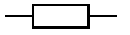
\includegraphics[width=0.15\columnwidth]{imgs/widerstand.pdf}
\end{figure}
\textbf{Formel:}
$$
	U = R ⋅ I
$$

\subsection{Kondensator}
\textbf{Schaltzeichen:} \\
\begin{figure}[H]
	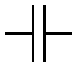
\includegraphics[width=0.1\columnwidth]{imgs/kondensator.pdf}
\end{figure}
\textbf{Formel:}
$$
	U = \frac 1 C \int I \textrm{ dt} \iff \dot U = \frac I C
$$

\subsection{Spule}
\textbf{Schaltzeichen:} \\
\begin{figure}[H]
	\includegraphics[width=0.1\columnwidth]{imgs/spule.pdf} bzw. 
	\includegraphics[width=0.1\columnwidth]{imgs/spule_alt.pdf}	
\end{figure}
\textbf{Formel:}
$$
	U = L ⋅ \dot I
$$

\subsection{Kirchoff'sches Spannungsgesetz}
In einem geschlossenen Stromkreis (Masche) ist die Summe aller Spannungen gleich null \\

\textbf{Beispiel:}
\begin{figure}[H]
	\includegraphics[width=0.5\columnwidth]{imgs/kvl.png}
\end{figure}
Für Masche $M_1$ gilt:
$$
U_R + U_C - U_e = 0
$$

\subsection{Kirchoff'sches Stromgesetz}
In jedem Knotenpunkt ist die Summe aller Ströme gleich null.

\textbf{Beispiel:}
\begin{figure}[H]
	\includegraphics[width=0.5\columnwidth]{imgs/kcl.png}
\end{figure}
$$
	I_C + I_L - I = 0
$$

\section{Physikalische Grundlagen}
\subsection{Kräfte}
\textbf{Kräftegleichgewicht:} \\
Die Summe aller Kräfte, die an einem Körper angreifen, addieren sich zu null.
$$
	\sum F_i = 0
$$

\textbf{Newtonsche Gesetze}
\begin{enumerate}
	\item Wirkt auf einen Körper keine Kraft oder befindet er sich im Kräftegleichgewicht, so bleibt er in Ruhe oder er bewegt sich mit konstanter Geschwindigkeit geradlinig weiter.
	\item $F = m ⋅ a$ \tab[2] ($m$: Masse des Körpers, $a$: Beschleunigung, die der Körper erfährt)
	\item $F_1 = -F_2$ \tab[2] (Kraft gleich Gegenkraft)
\end{enumerate}

\textbf{Masse-Feder-Dämpfer System}
\begin{figure}[H]
	\includegraphics[width=0.5\columnwidth]{imgs/mass-spring-damper.png}
\end{figure}
$m$: Masse des Körpers, $d$: Dämpferkonstante, $k$: Federkonstante, $F$: Stellkraft
$$
	F = m ⋅ \ddot x + d \dot x + k x
$$


\subsection{Drehmomente}
\textbf{Momentengleichgewicht:} \\
Die Summe aller Momente um jeden (einen) beliebigen Punkt eines Körpers addieren sich zu null.
$$
	\sum M_i = 0
$$

\textbf{Berechnung in Abhängigheit von F:} \\
$r$: Abstand der Wirkungslinie der Kraft von der Drehachse, $F$: wirkende Kraft
$$
	M = r \times F
$$

\subsection{Drehimpuls:}
$J$: Trägheitsmoment, $\omega$: Winkelgeschwindigkeit
$$
	L = J ⋅ \omega
$$

%TODO überarbeiten


\section{Tipps}
\subsection{Zeichnen eines Blockschaltbildes}
\begin{itemize}
	\item Verzweigungen von Signalen werden durch einen schwarzen Punkt markiert, um die Verwechslungsgefahr mit Kreuzungen ohne Kontakt zu vermeiden.
	\item Signale werden immer explizit mit Summationsgliedern aufaddiert.
	\item Proportionalitätsfaktoren von 1 können weggelassen werden.
	\item Das Vorzeichen beim Summationsglied steht immer rechts vom Pfeil. Die Pluszeichen müssen nicht explizit angegeben werden.
	\item Das Vorzeichen einer Rückführung steht am Soll-/Istwert-Vergleich
\end{itemize}
\textbf{Allgemeine Vorgehensweise:}
\begin{enumerate}
	\item Differentialgleichung nach höchster Ableitung auflösen
	\item $n$ I-Glieder mit zugehörigen Anfangswerten nebeneinander zeichnen, verbinden und beschriften
	\item Summationsglieder für die höchste Ableitung bilden
	\item Jeden Term der rechten Seite aus bestehenden Signalen bilden
\end{enumerate}

%TODO Impulsfunktion, Sprungfunktion

%TODO Beispiel




\pagebreak
\section*{Anmerkungen}
Dies ist eine Zusammenfassung der Vorlesung Regelungstechnik an der Technischen Universität München.
Gehalten wurde diese Vorlesung durch Lohmann B. im Sommersemester 2019.
Ersteller dieser Zusammenfassung ist Gaida B.
Alle Angaben sind ohne Gewähr.


\section*{Literaturverzeichnis}
Werner Skolaut. \textit{Maschinenbau. Ein Lehrbuch für das ganze Bachelor-Studium}. Springer Vieweg. Heidelberg, 2018, S. 1271 - 1387





\end{document}

%TODO check for todos








